\documentclass[10pt]{book}
\usepackage[utf8]{inputenc}
\usepackage[a4paper]{geometry}
\usepackage{fix-cm}
\usepackage{chngpage}
\usepackage{graphicx}
\usepackage{color}
\usepackage{makeidx}
\usepackage{longtable}
\usepackage{colortbl}
\usepackage[table]{xcolor}
\usepackage{underscore}
\usepackage{caption}
\usepackage{amsmath}
\usepackage{float}
\usepackage{array}
\usepackage{datatool}
\usepackage{subfigure}
\usepackage{fancyhdr}
\usepackage[Bjarne]{fncychap}
\usepackage{listings}
\usepackage{bold-extra}
\usepackage{lettrine}
\usepackage{booktabs}
\usepackage{multirow}
\definecolor{seagreen}{RGB}{64,100,120}
\definecolor{darkpink}{RGB}{200,100,120}
\definecolor{light-gray}{gray}{0.85}
\definecolor{medium-gray}{gray}{0.5}
\usepackage[colorlinks=true,linkcolor=seagreen,citecolor=darkpink]{hyperref}
\usepackage{path}
\usepackage{tikz}
\usepackage[most]{tcolorbox}


%
% custom options
%
\renewcommand{\captionlabelfont}{\small \bf}
\renewcommand{\captionfont}{\small \it}
\setlength{\parindent}{0mm}
\setlength{\parskip}{.5\baselineskip}
\fancyhead{} % clear all header fields
\fancyhead[RO,LE]{\thepage}
\fancyhead[LO,RE]{\nouppercase{\rightmark}}
\fancyfoot{} % clear all footer fields
%\fancyfoot[LO,RE]{\slshape The Trampoline Handbook}
\fancyfoot[RO,LE]{\slshape\nouppercase{\leftmark}}
\renewcommand{\headrulewidth}{0.4pt}
\renewcommand{\footrulewidth}{0.4pt}
\pagestyle{fancy}
\ChTitleVar{\raggedleft\Huge\sffamily}
\ChNameVar{\raggedleft\normalsize\sffamily}
\ChNumVar{\raggedleft\bfseries\Large\sffamily}

%
% C language options
%
\lstset{
  language=C,
  basicstyle=\ttfamily\footnotesize,
  commentstyle=\itshape\color{cyan}
}

%
% OIL language options
%
\lstdefinelanguage{OIL}
{
  morekeywords= {
  	  APPMODE,
	  BUILD,
	  STATUS,
	  APP_SRC, 
	  TRAMPOLINE_BASE_PATH,
	  LDFLAGS,
	  APP_NAME,
	  OIL_VERSION,
	  SYSTEM,
	  TRUE,
	  EXTENDED,
	  AUTOSTART,
	  ACTIVATION,
	  IMPLEMENTATION,
	  RESOURCE, RESOURCEPROPERTY, STANDARD, INTERNAL, LINKED, LINKEDRESOURCE,
	  TASK, SCHEDULE, FULL, NONE, PRIORITY, EVENT, ISR, CATEGORY, OS, CPU, MEMMAP,
	  COMPILER, LINKER, SCRIPT, IOC, DATATYPENAME, DATATYPEPROPERTY, RECEIVER, SENDER, RCV_OSAPPLICATION, 	  RECEIVER_PULL_CB, ACTION, SENDER_ID, SND_OSAPPLICATION
	}
}

\lstset{
  language=OIL,
%  emph={
%    var,
%    expression,
%    string,
%    instruction_list,
%    template_file_name,
%    reader,
%    hierarchy
%  },
  emphstyle=\em,
  moredelim=[s]{"}{"},
  basicstyle=\ttfamily\small}

\lstdefinelanguage{goilTemplate}
{
  morekeywords= {
	  after,
	  before,
	  between,
	  block,
	  default,
	  do,
	  else,
	  elsif,
	  emptylist,
	  end,
	  error,
	  exists,
	  false,
	  for,
	  foreach,
	  from,
	  here,
	  let,
	  loop,
	  no,
	  if,
	  in,
	  mod,
	  not,
	  or,
	  prefixedby,
	  template,
	  then,
	  to,
	  true,
	  yes,
	  warning,
	  while,
	  write,
	  !,
	  ?
	}
}

\lstset{
  language=goilTemplate,
  emph={
    var,
    expression,
    string,
    instruction_list,
    template_file_name,
    reader,
    hierarchy
  },
  emphstyle=\em,
  moredelim=[s][\color{blue}]{\%}{\%},
  moredelim=[s]{"}{"},
  morecomment=[l][\color{medium-gray}\itshape]{\#},
  basicstyle=\ttfamily\small,
  morekeywords=\bfseries
}

% Inline color boxes

\newtcbox{\inlinebox}[1][red]{
	on line,
	arc=0pt,
	outer arc=0pt,
	colback=#1!10!white,
	colframe=#1!50!black,
	boxsep=0pt,
	left=2pt,
	right=2pt,
	top=1pt,
	bottom=1pt,
	boxrule=.25pt
}

%
% Commands for paragraph types
%
%\newcommand{\note}[1]{\vspace{1mm}\fbox{\begin{minipage}[t]{.1\linewidth}{\bfseries Note:}\end{minipage}%
%\hfill\begin{minipage}[t]{.885\linewidth}#1\end{minipage}}\vspace{1mm}}
\newcommand{\note}[1]{%
\hspace{-12.4mm}
\rowcolors{1}{white}{white}
\begin{tabular}[b]{m{5mm}|m{\linewidth}}

\includegraphics[width=6mm,angle=45]{pictures/note} & #1\\
\end{tabular}
}
\newcommand{\warning}[1]{%
\hspace{-14.2mm}
\rowcolors{1}{white}{light-gray}
\begin{tabular}[b]{m{7mm}|m{\linewidth}}

\includegraphics[width=7mm]{pictures/warn} & #1\\
\end{tabular}
}
%
% Commands for inline formatting of C computing language
%
\newcommand{\argu}[1]{{\ttfamily #1}}
\newcommand{\ctype}[1]{{\small\ttfamily #1}}
\newcommand{\cdata}[1]{{\ttfamily #1}}
\newcommand{\var}[1]{{\ttfamily\em #1}}
\newcommand{\va}{\small\ttfamily\em}
\newcommand{\cfunction}[1]{{\ttfamily #1}}
\newcommand{\cmacro}[1]{{\small\ttfamily #1}}
\newcommand{\constant}[1]{{\small\ttfamily #1}}
\newcommand{\oilobj}[1]{\lstinline[language=OIL]{#1}}
\newcommand{\oilattr}[1]{\lstinline[language=OIL]{#1}}
\newcommand{\oilval}[1]{\lstinline[language=OIL]{#1}}
\newcommand{\member}[1]{{\small\ttfamily #1}}
\newcommand{\mem}{\small\ttfamily}

%
% Commands for other formatting
%
\newcommand{\tool}[1]{{\small\ttfamily #1}}
\newcommand{\com}[1]{\inlinebox[blue]{\small\ttfamily #1}}
\newcommand{\file}[1]{{\small\ttfamily `#1'}}
\newcommand{\envvar}[1]{{\scriptsize\sffamily #1}}
\newcommand{\longprogramopt}[1]{{\small\ttfamily --#1}}
\newcommand{\programopt}[1]{{\ttfamily -#1}}
\newcommand{\strong}[1]{{\bf #1}}
\newcommand{\ie}{i.e.}
\newcommand{\asfct}[1]{\texttt{#1}}
\newcommand{\hex}[1]{\texttt{#1$_H$}}
\newcommand{\reg}[1]{\textit{#1}}
\newcommand{\dreg}[1]{{\small\ttfamily #1}}
\newcommand{\idxconfflag}[1]{{\footnotesize\ttfamily #1}\index{Configuration macros!#1}\index{#1}}
\newcommand{\toreplace}[1]{{\footnotesize $<$}#1{\footnotesize $>$}}
%\newcommand{\figcaption}[2]{\textit{\caption{\small #1}}\label{#2}}
\newcommand{\goil}{\tool{goil}\index{goil, The OIL/arXML compiler of Trampoline}}
\newcommand{\process}{process\index{process, a task, basic or extended, or an ISR category 2}}
\newcommand{\sysgen}{system generation tool\index{system generation tool, the tool that takes as an input a description of the system (in OIL or in XML) to generate the corresponding .c and .h files.}}
\newcommand{\stringlit}[1]{{\small\ttfamily "{#1}"}}
\newcommand{\character}[1]{{\small\ttfamily `{#1}'}}
\newcommand{\api}[1]{\cfunction{#1}\index{#1}}
\newcommand{\osek}{OSEK}
\newcommand{\autosar}{{\small AUTOSAR}}
\newenvironment{penum}{
\begin{enumerate}
  \setlength{\itemsep}{1pt}
  \setlength{\parskip}{0pt}
  \setlength{\parsep}{0pt}
}{\end{enumerate}}
\newenvironment{pitemize}{
\begin{itemize}
  \setlength{\itemsep}{1pt}
  \setlength{\parskip}{0pt}
  \setlength{\parsep}{0pt}
}{\end{itemize}}

%
% Graphic symbols for scheduling diagrams
%
\newcommand{\activate}{
\includegraphics[height=9pt]{pictures/activate.pdf}}
\newcommand{\terminate}{
\includegraphics[height=9pt]{pictures/terminate.pdf}}

%
% states of a task
%
\newcommand{\RUNNING}{\constant{RUNNING}\index{RUNNING, state of a task}}
\newcommand{\READY}{\constant{READY}\index{READY, state of a task}}
\newcommand{\SUSPENDED}{\constant{SUSPENDED}\index{SUSPENDED, state of a task}}
\newcommand{\WAITING}{\constant{WAITING}\index{WAITING, state of a task}}
\newcommand{\AUTOSTART}{\constant{AUTOSTART}\index{AUTOSTART, state of a task}}
\newcommand{\READYANDNEW}{\constant{READY\_AND\_NEW}\index{READY_AND_NEW, state of a task}}

%
% Kind of task
%
\newcommand{\BASIC}{\constant{BASIC}\index{BASIC, compilation with no extended error checking}}
\newcommand{\EXTENDED}{\constant{EXTENDED}\index{EXTENDED, compilation with extended error checking}}

%
% result codes
%
\newcommand{\OK}{E\_OK}
\newcommand{\OSID}{E\_OS\_ID}
\newcommand{\OSLIMIT}{E\_OS\_LIMIT}
\newcommand{\OSRESOURCE}{E\_OS\_RESOURCE}
\newcommand{\OSCALLLEVEL}{E\_OS\_CALLEVEL}
\newcommand{\OSPROTECTIONMEMORY}{E\_OS\_PROTECTION\_MEMORY}
\newcommand{\OSACCESS}{E\_OS\_ACCESS}
\newcommand{\OSSTATE}{E\_OS\_STATE}

%
% Scalability class
%
\newcommand{\SC}[1]{scalability class #1}

%
% OIL attribute
%
\newcommand{\PRIORITY}{PRIORITY\index{PRIORITY}}
\newcommand{\SCHEDULE}{SCHEDULE\index{SCHEDULE}}
\newcommand{\TRUE}{{\small\ttfamily TRUE}}
\newcommand{\FALSE}{{\small\ttfamily FALSE}}

%
% Conf macros
%
\newcommand{\YES}{{\small\ttfamily YES}}
\newcommand{\NO}{{\small\ttfamily NO}}

%
% environment and commands to describe system services
%
\newcommand{\servicename}{}
\newcommand{\apiname}{}
\newcommand{\servicedescription}{}
\newcommand{\servicereturn}{}
\DTLnewdb{argDB}
\DTLnewdb{resDB}
\newenvironment{service}[2]{%
  \subsection{#1}\label{api:#1}\index{#1}%
  \renewcommand{\servicename}{#1}%
  \renewcommand{\apiname}{\api{#1}}%
  \renewcommand{\servicereturn}{#2}
  \DTLcleardb{argDB}
  \DTLcleardb{resDB}
}{
 
%  \vspace{1mm}
  {\bf Prototype of \servicename:}\nopagebreak
  
  {\tt\if\servicereturn\empty\relax\else\servicereturn\ \fi}{\tt \servicename(%
  \DTLifdbempty{argDB}{void}{%
    \DTLforeach*{argDB}{\argumenttype=type,\argumentname=name}{%
      \DTLiffirstrow{}{, }\argumenttype\ \argumentname%
    }%
  });}

  \DTLifdbempty{argDB}{}{
%    \vspace{1mm}
    {\bf Arguments of \servicename:}\nopagebreak
  
    \DTLforeach*{argDB}{\argumenttype=type,\argumentname=name,\argumentdesc=desc}{%
      \par\begingroup\hangindent=2em\hangafter=1 {\ttfamily\argumentname}\hspace{1em}\argumentdesc.\par\endgroup
    }
  }
  
  \DTLifdbempty{resDB}{}{
%    \vspace{1mm}
    {\bf Status codes returned by \servicename:}\nopagebreak
  
    \DTLforeach*{resDB}{\statusres=value,\statusdesc=desc,\statusstatus=status}{%
      \par\begingroup\hangindent=2em\hangafter=1 {\ttfamily\statusres}\hspace{1em}\statusdesc\ (\statusstatus).\par\endgroup
    }
  }
}

\newcommand{\argument}[3]{%
  \DTLnewrow{argDB}
  \DTLnewdbentry{argDB}{type}{#1}
  \DTLnewdbentry{argDB}{name}{#2}
  \DTLnewdbentry{argDB}{desc}{#3}
}

\newcommand{\resultcode}[2]{%
  \DTLnewrow{resDB}
  \DTLnewdbentry{resDB}{value}{#1}
  \DTLnewdbentry{resDB}{desc}{#2}
  \DTLnewdbentry{resDB}{status}{extended and standard}
}
  
\newcommand{\resultcodeauto}[2]{%
  \DTLnewrow{resDB}
  \DTLnewdbentry{resDB}{value}{#1}
  \DTLnewdbentry{resDB}{desc}{#2}
  \DTLnewdbentry{resDB}{status}{\AUTOSAR, extended and standard}
}
  
\newcommand{\resultcodeext}[2]{%
  \DTLnewrow{resDB}
  \DTLnewdbentry{resDB}{value}{#1}
  \DTLnewdbentry{resDB}{desc}{#2}
  \DTLnewdbentry{resDB}{status}{extended only}
}

\newcommand{\resultcodeautoext}[2]{%
  \DTLnewrow{resDB}
  \DTLnewdbentry{resDB}{value}{#1}
  \DTLnewdbentry{resDB}{desc}{#2}
  \DTLnewdbentry{resDB}{status}{\AUTOSAR, extended only}
}

\newcommand{\resultcodeMP}[2]{%
  \DTLnewrow{resDB}
  \DTLnewdbentry{resDB}{value}{#1}
  \DTLnewdbentry{resDB}{desc}{#2}
  \DTLnewdbentry{resDB}{status}{extended + \autosar\ \SC{3} and \SC{4} only}
}

%
% sorted table
%
\DTLnewdb{tableDB}
\newenvironment{sortedtable}[1]{%
  \DTLcleardb{tableDB}
  \begin{longtable}{#1}
}{
\DTLsort*{name}{tableDB}%
\DTLforeach*{tableDB}{%
\colname=name,\coltype=type,\coldesc=desc}{%
\DTLiffirstrow{\\\hline\endhead}{\\}%
\colname&\coltype&\coldesc}%
\end{longtable}
%\DTLdisplaylongdb{tableDB}
}
\newcommand{\sortline}[3]{%
  \DTLnewrow{tableDB}%
  \DTLnewdbentry{tableDB}{name}{#1}%
  \DTLnewdbentry{tableDB}{type}{#2}%
  \DTLnewdbentry{tableDB}{desc}{#3}%
}
%
% Here we go
%

%\includeonly{porting}

\title{The Trampoline handbook}
\author{Jean-Luc B\'echennec\\Florent Pavin\\Pierre Molinaro}

\makeindex

\begin{document}
\begin{titlepage}
\begin{tikzpicture}[remember picture,overlay]
\node (background) at (0.55\textwidth,-0.7\textheight) {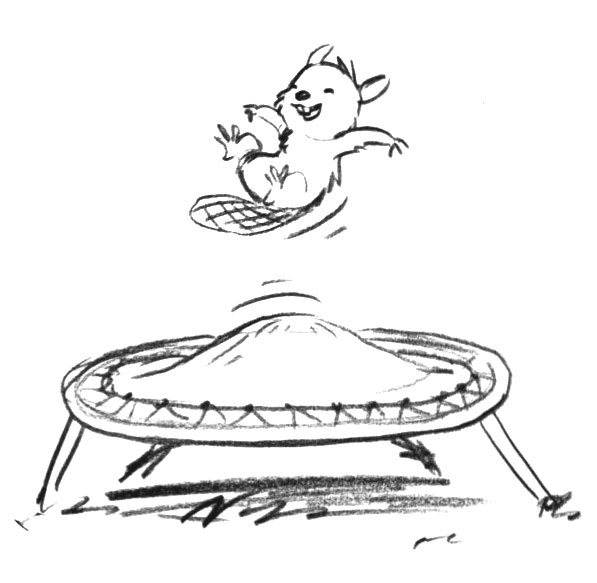
\includegraphics[scale=.5]{trampolineBeaver.jpg}};
\end{tikzpicture}
\begin{minipage}[t]{1.1\linewidth}
\rule{\linewidth}{3pt}
\fontsize{40}{42}\selectfont\raggedleft\sffamily\bfseries The Trampoline Handbook

\vspace{2cm}\Large release 2.0

\vspace{2cm}
\large
Jean-Luc Béchennec\\
Mikaël Briday\\
Sébastien Faucou\\
Pierre Molinaro\\
Florent Pavin\\
\end{minipage}
\end{titlepage}
\setcounter{tocdepth}{2}
\tableofcontents


\part{The Real-Time Operating System}
%!TEX root = ./main.tex

\chapter{Getting started}

This chapter shows how to compile and run your first application. We are going to use the \textsc{Posix} port of Trampoline, Trampoline/\textsc{Posix}, that runs over a Linux or Mac OS X operating system. So it is assumed you are using a Linux or Mac OS X computer since Trampoline/Posix does not run over Windows\footnote{An API working like Unix signals is missing on Windows.}. It is also assumed that you have a basic knowledge of using the command line and the Unix shell.

OSEK/VDX and \textsc{Autosar os} are static operating systems. That means the objects of the application, tasks, events, resources, \ldots, cannot be created or deleted during the execution of the application. All objects are statically defined and instead of forcing the user to instantiate the OS objects related to the application in C language, a work that can be error prone, a specific language is used, OIL or XML\footnote{for \textsc{Autosar}}. A compiler, \goil, is used to translate the description in the equivalent C structures. \goil\ performs verifications too.

\section{Setting up the environment}

Before compiling and running the first application, a few tools are required. The first tool needed is a development chain, compiler and linker, for the target platform. In our case, the native development chain, \tool{gcc} under Linux, \tool{clang} under Mac OS X will be used. The two other tools are respectively \goil\ and \tool{viper} that we will compile. In the following, all paths are relative to the Trampoline root directory. When setting up path environment variables, complete the relative path with the installation path of Trampoline.

\subsection{Compiling goil}

\goil\ is located in the \file{goil} subdirectory. To compile \goil, go in the directory corresponding to your operating system, \file{goil/makefile-macosx} for Mac OS X or \file{goil/makefile-unix} for Linux. Then type \com{./build.py release}. If everything went well, a \goil\ executable is generated. You can test it by typing \com{./goil --version}. At the time of writing, the command should output:

\begin{verbatim}
alflolol:makefile-macosx jlb$ ./goil --version
goil : 3.1.11, build with GALGAS 3.3.11
No warning, no error.
\end{verbatim}

You can install \tool{goil} in \file{/usr/local/bin} by typing \com{sudo ./build.py install-release} or you can add to your \envvar{PATH} environment variable the location where \goil\ has been compiled.

In addition you may want to set up the \envvar{GOIL_TEMPLATES} environment variable in your \file{.profile} or \file{.bashrc} so that you don't always have to set the \longprogramopt{templates=} option when calling \tool{goil}. This variable stores the path to the templates directory used by \tool{goil} and shall be \file{goil/templates}.

\subsection{Compiling viper}

Under Posix, Trampoline requires a runtime support that mimics the minimum behavior of a hardware, mainly timers. \tool{viper} is a separate application used by Trampoline for this purpose. Go in the \file{viper} directory. Type \com{make} to compile \tool{viper}. You must also set the environment variable \envvar{VIPER_PATH} to contain the path \file{viper}.

\section{Playing with the \cdata{one_task} application}

Go into the \file{examples/posix/one_task} directory. In this directory, two files are available: \file{one_task.oil} and \file{one_task.c}. Start by opening \file{one_task.oil}. The content of this file is reproduced below. 

\begin{lstlisting}[language=OIL,numbers=left,escapechar=?]
OIL_VERSION = "2.5"; 	?\label{onetask::oilversion}?

CPU only_one_task {  	?\label{onetask::cpu}?
  OS config {			?\label{onetask::cpu::os}?
    STATUS = EXTENDED;
    BUILD = TRUE { ?\label{onetask::cpu::os::build}?
      APP_SRC = "one_task.c";
      TRAMPOLINE_BASE_PATH = "../../..";
      LDFLAGS="-lrt -lpthread";
      APP_NAME = "one_task_exe";
      LINKER = "gcc";
      SYSTEM = PYTHON;
    };
  };
  
  APPMODE stdAppmode {}; ?\label{onetask::cpu::appmode}?
  
  TASK my_only_task {
    PRIORITY = 1;
    AUTOSTART = TRUE { APPMODE = stdAppmode; };
    ACTIVATION = 1;
    SCHEDULE = FULL;
  };
};
\end{lstlisting}

\lstinline[language=OIL]{OIL_VERSION = "2.5";} at line~\ref{onetask::oilversion} specifies which kind of application we are designing. Here it is an \osek\ application. For an \autosar\ application, \lstinline[language=OIL]{OIL_VERSION = "4.0";} would be used.

OIL files consist of two sections, an \oilobj{IMPLEMENTATION} section that is not used here and a \oilobj{CPU} section that appears in the line \ref{onetask::cpu}. The objects describing the application are located inside the \oilobj{CPU} section.

The first is the \oilobj{OS} object at the line~\ref{onetask::cpu::os}. This object is used to configure the operating system and, in the case of Trampoline, to specify how to compile it. The first attribute, \oilattr{STATUS}, indicates the fineness of verification of error conditions by the operating system services. Two values are possible: \oilval{STANDARD} and \oilval{EXTENDED}. Here, \oilval{EXTENDED} is used.

The \oilattr{BUILD} attribute at line~\ref{onetask::cpu::os::build} is used to generate a build script. It contains several sub-attributes:
\begin{itemize}
\item \oilattr{APP_SRC} gives the C source code file of your application. If the application is split into several C files, use has many \oilattr{APP_SRC} as needed.
\item \oilattr{TRAMPOLINE_BASE_PATH} gives the path to the Trampoline root directory.
\item \oilattr{LDFLAGS} is additional flags to pass to the linker. Here we add the \emph{rt} and \emph{pthread} libraries that are needed for multitasking and communication with \tool{viper}. 
\item \oilattr{APP_NAME} is the name of the resulting binary file that is directly executable for the Posix target.
\item \oilattr{LINKER} specifies which command is used to invoke the linker.
\item \oilattr{SYSTEM} specifies which build system is used. Here Python build scripts.
\end{itemize}

The second is the object \oilobj{APPMODE} at line~\ref{onetask::cpu::appmode}
%!TEX root = ./main.tex

\chapter{Operating System Execution}
\label{chap:appmodes}

\lettrine{T}his chapter presents how to start and shutdown the operating system as well as the configuration options and the Application Modes. Application Modes are used to start the operating system in different configurations. Usually, the configuration is read from hardware switches. The current Application Mode is passed to the \api{StartOS} service and cannot be changed once the operating system is started. 

\section{Configuration Options}

\section{System Services}

\begin{service}{StartOS}{void}
\argument{AppModeType}{AppModeID}{The Application Mode}

\apiname\ starts the OS in the \argu{AppModeID} Application Mode. First the OS does some initializations, then the Startup Hook, if configured, is called. At last the scheduling is started and the highest priority task runs.

\note{When called from outside a task or an ISR, typically from the \cfunction{main()}, \apiname\ does not returns. When called from a task or an ISR, a case which is forbidden, \apiname\ returns and the Error Hook (if configured) is called.}

\warning{If \argu{AppModeID} does not correspond to any Application Mode, no error occurs but none of the \oilattr{AUTOSTART} objects is started.}

\end{service}

\begin{service}{ShutdownOS}{void}
\argument{StatusType}{Error}{The error that occurred}

\apiname\ shuts down the OS and notify the \argu{Error} error code. If it is configured, the Shutdown Hook is called with \argu{Error} as argument. The behavior may depends on the target platform. On embedded platforms interrupts are disabled and an infinite loop or a \asfct{halt} is executed. On POSIX the application exits.

\end{service}

\section{Application Modes Declarations}
\label{sec:appmodedec}

Application Mode are used to specify which \oilattr{AUTOSTART} objects (tasks, alarms or schedule tables) are started when \api{StartOS} is called. Application Modes are declared in OIL using the \oilobj{APPMODE} object. \goil\ accepts the \oilattr{DEFAULT} boolean attribute. When \oilval{TRUE}, this attributes specifies the default Application Mode. \oilattr{DEFAULT} is implicitly \oilval{FALSE}.

When only one Application Mode is defined, the constant \constant{OSDEFAULTAPPMODE} is set to this Application Mode. When more than one Application Mode are defined, one and only one of the Application Modes \oilattr{DEFAULT}  attribute must be set to \oilval{TRUE} and the constant \constant{OSDEFAULTAPPMODE} is set to this one.

At most 32 application modes may be declared in the current implementation. We believe it is far enough.

In the following example, 2 Application Modes are declared:

\begin{lstlisting}[language=OIL]
APPMODE normal { DEFAULT = TRUE; };

APPMODE diag { };
\end{lstlisting}

Let's consider 2 tasks and one alarm. The first task, {\em command}, is \oilattr{AUTOSTART} in any case, the second one, {\em logging} is not \oilattr{AUTOSTART} and the alarm, {\em trigger_logging}, is \oilattr{AUTOSTART} in Application Mode \constant{diag} only. The goal is to have a periodic task doing some logging when the OS is started in Application Mode \constant{diag}:

\begin{lstlisting}[language=OIL]
TASK command {
  AUTOSTART = TRUE {
    APPMODE = normal;
    APPMODE = diag;
  };
  ...
};

TASK logging {
  AUTOSTART = FALSE;
  ...
};

ALARM trigger_logging {
  AUTOSTART = TRUE {
    APPMODE = diag;
    ALARMTIME = 10;
    CYCLETIME = 10;
  };
  ACTION = ACTIVATETASK {
    TASK = logging;
  };
  ...
};
\end{lstlisting}

If \api{StartOS} is called with argument \constant{normal} or \constant{OSDEFAULTAPPMODE}, the alarm {\em trigger_logging} is not started by \api{StartOS} and task {\em logging} does not run. If \api{StartOS} is called with argument \constant{diag}, the alarm is started and task {\em logging} runs. In both cases task {\em command} is started.

\section{Application Modes Services}

\begin{service}{DeclareApplicationMode}{}
\argument{AppModeType}{AppModeID}{The Application Mode}

On the C side, each declared Application Mode is available as a constant of type \ctype{AppModeType}. However, before using one of the constants, you have to put it in the current scope with the \servicename\ service\,\footnote{This macro is not part of \cite{OSEKOS223} but has been added for convenience purpose}  as follow:

\begin{lstlisting}[language=C]
DeclareApplicationMode(normal);
DeclareApplicationMode(diag);
\end{lstlisting}

An exception is the constant \constant{OSDEFAULTAPPMODE} which is in the scope as long as file \file{tpl_os.h} is included.

\note{\apiname\ is a C macro}
\end{service}

\begin{service}{GetActiveApplicationMode}{AppModeType}
\api{GetActiveApplicationMode} returns the Application Mode that was used to start the OS.
\begin{lstlisting}[language=C]
AppModeType currentAppMode;
currentAppMode = GetActiveApplicationMode();
\end{lstlisting}
If \apiname\ is called before the OS is started, \constant{OSNOAPPMODE} is returned.

\end{service}

\section{Implementation}

At system generation time, an identifier \constant{AppModeID} of type \ctype{AppModeType} is attributed to each Application Mode.
Identifiers range from $0$ to $number~of~application~modes - 1$ and are attributed by \goil\ in their order of appearance in the OIL file.

For each \constant{AppModeID}, \goil\ computes a mask: \lstinline[language=OIL]{AppModeMask = 1 << AppModeID}.
For each task, alarm and schedule table, a table indexed by the object id is computed by \goil. Each element of these tables is the bitwise or of the \constant{AppModeMask} in which the object is \oilattr{AUTOSTART}. If there is no task, alarm or schedule table defined, the corresponding table is not generated.


\api{StartOS} iterates over the tasks, alarms and schedule tables Application Mode mask tables. It does a bitwise and with the mask stored in the table and the mask computed from the Application Mode. If the result is not 0 then the corresponding object is \oilattr{AUTOSTART}  in this Application Mode and is started.

Using the example of section \ref{sec:appmodedec} we have

\begin{lstlisting}[language=C]
CONST(tpl_application_mode, OS_CONST) diag = 0; /* mask = 1 */
CONST(tpl_application_mode, OS_CONST) normal = 1; /* mask = 2 */
\end{lstlisting}

\ctype{AppModeType} is an alias of \ctype{tpl_application_mode}. 

\begin{lstlisting}[language=C]
CONST(tpl_appmode_mask, OS_CONST) tpl_task_app_mode[TASK_COUNT] = {
  3 /* task command : normal | diag */ ,
  0 /* task logging :  */ 
};

CONST(tpl_appmode_mask, OS_CONST) tpl_alarm_app_mode[ALARM_COUNT] = {
  1 /* alarm trigger_logging : diag */ 
};
\end{lstlisting}

The \ctype{tpl_appmode_mask} type is computed according to the number of Application Modes.

\begin{table}[htbp]
\caption{Size of \ctype{tpl_appmode_mask} type.}
\rowcolors{1}{white}{light-gray}
\begin{longtable}[c]{c|c}
\bf Number of Application Modes & \bf \ctype{tpl_appmode_mask} type\\
\hline
$[ 1, 8]$ & \ctype{u8}\\
$[ 9, 16]$ & \ctype{u16}\\
$[ 17, 32]$ & \ctype{u32}\\
\end{longtable}
\label{tab:statetrans}
\end{table}


%!TEX root = ./main.tex

\chapter{Tasks}
\label{chap:tasks}

\lettrine{A} task is an execution framework for the functions of the application\,\footnote{The term {\em Application} is also used in \autosar\ to designate a set of object, this manual uses OS Application to name the \autosar\ applications and Application to name the user level software.}. A task is a kind of \process. Tasks are executed concurrently and asynchronously, see \ref{sec:scheduling}. 2 kinds of task exist: basic tasks and extended tasks. A basic task cannot block (\ie\ it cannot use a service that may block) while an extended task can.
The tasks and their properties are declared in the OIL file, see \ref{oil:task}. Their functions are defined in a C file.

\section{States a task}
\label{sec:taskstate}

A task may be in different states. A basic task may be currently executing (in the \RUNNING\ state), ready to execute (in the \READY\ state) or not active at all (in the \SUSPENDED\ state). Figure \ref{fig:basictaskstates} shows the states of a basic task. An extended task has an additional \WAITING\ state.  Figure \ref{fig:extendedtaskstates} shows the states of an extended task. See section \ref{sec:internaltaskstate} for additional informations about the states of a task.

\begin{figure}[htbp] %  figure placement: here, top, bottom, or page
   \centering
   \parbox{.45\linewidth}{%
     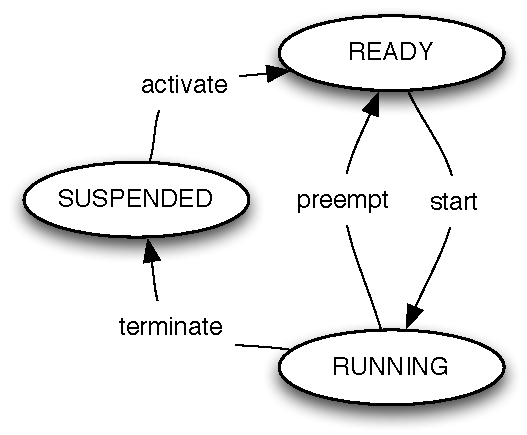
\includegraphics[scale=.6]{pictures/statesBasic.pdf} 
     \caption{States of a \BASIC\ task.}%
     \label{fig:basictaskstates}}%
%   \qquad
   \begin{minipage}{.55\linewidth}%
     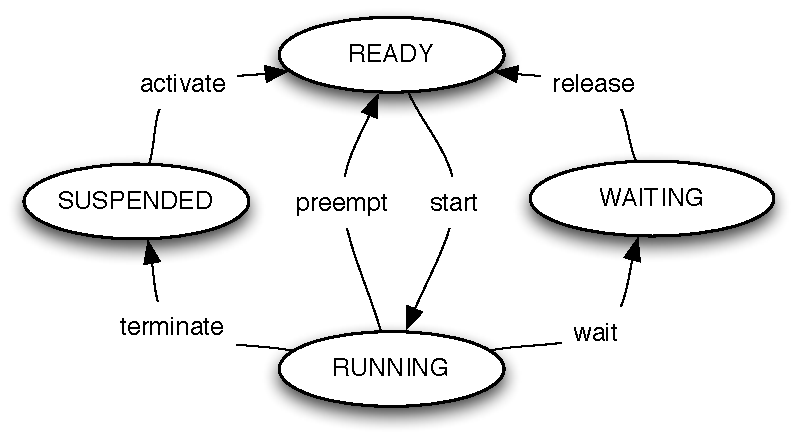
\includegraphics[scale=.6]{pictures/statesExtended.pdf} 
     \caption{States of an \EXTENDED\ task.}%
     \label{fig:extendedtaskstates}%
   \end{minipage}%
\end{figure} 


A task goes from one state to the other according to various conditions as shown in table \ref{tab:statetrans}.

\begin{table}[htbp]
\caption{Transition from state to state of a task.}
\rowcolors{1}{white}{light-gray}
\begin{longtable}[c]{l|l|l|p{7cm}}
\bf transition & \bf former state & \bf new state & \bf description\\
\hline
activate & \SUSPENDED & \READY & the task is set in the \READY\ state on one of the following occurrences: services \api{ActivateTask} or \api{ChainTask}, activation notification coming from an alarm, a schedule table or a message. \\
start & \READY & \RUNNING & the task is set to the running state and begin to execute because it has the highest priority in the system and has been elected by the scheduler. \\
terminate & \RUNNING & \SUSPENDED & the task is set to the \SUSPENDED\ state when it calls the \api{TerminateTask} or \api{ChainTask} service.\\
preempt & \RUNNING & \READY & the task is set to the \READY\ state when the scheduler starts a higher priority task.\\
wait & \RUNNING & \WAITING & the task may be set to the \WAITING\ state when it calls the service \api{WaitEvent}.\\
release & \WAITING & \READY & the task is set to the \READY\ state when it gets one of the  events it is waiting for. \\
\end{longtable}
\label{tab:statetrans}
\end{table}

\note{A system service may do more than one transition at a time. For instance, if a task is activated by calling \cfunction{ActivateTask} and its priority is higher than the priority of the current running task, the new task will go from \SUSPENDED\ to \RUNNING\ and the intermediate state \READY\ will not be observable.}

\section{The scheduling}
\label{sec:scheduling}

Trampoline schedules the tasks dynamically during the execution of the application. A task is scheduled according to its priority and whether it is preemptable or not. The priority of a task is given at design stage, and indicated in the OIL file using the \PRIORITY\ attribute, see \ref{sec:oiltask}, and may change during execution when the task gets or release a resource. The preemptability of a task may be set too. It is also indicated in the OIL file using the \SCHEDULE\ attribute, see \ref{sec:oiltask}.

A tasks continues to run until it is preempted because a task having a higher priority is put in the \READY\ state,  or it blocks because it is waiting for an event. Only extended tasks may block. If more than one task have the same priority, tasks are run one after the other because a task may not preempt an other task having the same priority. So there is no round robin among tasks of the same priority level.

A non-preemptable task runs until it calls \api{Schedule} and a higher priority task is in the \READY\ state or until it blocks. More informations about priority and preemptability may be found in chapter \ref{chap:resources}.

In the following examples, the horizontal axis is the time.  The state of the task is indicated in a rectangle that spans a period of time. When the task is running the rectangle is grayed. An up arrow \activate\ indicates a task activation and a down arrow \terminate\ a task termination.

\begin{figure}[htbp] %  figure placement: here, top, bottom, or page
   \centering
   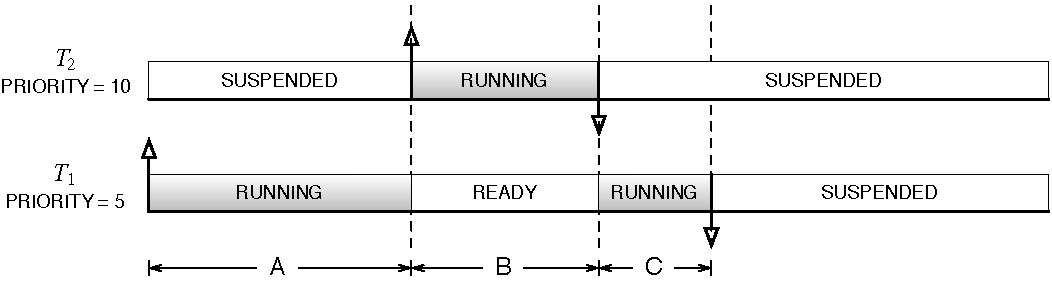
\includegraphics[scale=.7]{pictures/schedulingPreempt.pdf} 
   \caption{{\bfseries Scheduling of preemptable tasks.} During A period, $T_1$ is {\sffamily\scshape running} and $T_2$ is {\sffamily\scshape suspended}. Then $T_2$ is activated. Since $Prio(T_2) > Prio(T_1)$, $T_1$ is preempted and $T_2$ runs (B period). $T_2$ terminates and $T_1$ becomes {\sffamily\scshape running} again (C period) until it terminates.}
   \label{fig:schedulePreempt}
\end{figure} 

\begin{figure}[htbp] %  figure placement: here, top, bottom, or page
   \centering
   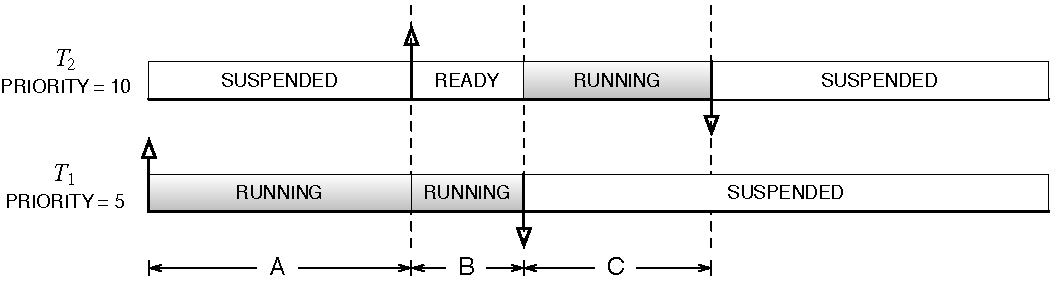
\includegraphics[scale=.7]{pictures/schedulingNonPreempt.pdf} 
   \caption{{\bfseries Scheduling of non-preemptable tasks.} During A period, $T_1$ is {\sffamily\scshape running} and $T_2$ is {\sffamily\scshape suspended}. Then $T_2$ is activated. Even if $Prio(T_2) > Prio(T_1)$, $T_1$ is non-preemptable and continues to run until it terminates (B period). In the meantime, $T_2$ is {\sffamily\scshape ready}. $T_1$ terminates and $T_2$ runs (C period) until it terminates.}
   \label{fig:schedulePreempt}
\end{figure} 

\section{Writing the code of a task}

Trampoline provides a \cmacro{TASK} macro to define a task in a C source file. The macro takes one argument which is the identifier of the task:

%\newpage
\begin{lstlisting}[language=C]
TASK(MyTask)
{
  /* code of the task */
  
  TerminateTask();
}
\end{lstlisting}

The code of the task is plain C.

The task should always end with a call to the \api{TerminateTask} service. See \ref{api:TerminateTask}.


\section{Tasks services}

\begin{service}{DeclareTask}{}

Each task has an identifier of type \ctype{TaskType}. This identifier is declared in the OIL file and is used in system calls to refer to a particular task. Before using such an identifier in your program, you have to declare it:

\begin{lstlisting}[language=C]
DeclareTask(MyTask);
\end{lstlisting}

This makes the \cdata{MyTask} identifier available in the current scope.

\note{ \servicename\ is a C macro. When the task has been define above using the macro \cmacro{TASK}, the identifier of the task is already in the scope and \cmacro{DeclareTask} is not needed.}

\argument{TaskType}{TaskID}{The id of the task to declare}
\end{service}

\begin{service}{ActivateTask}{StatusType}

\note{This service does a rescheduling}

Activates a new instance of a task. If activation counter has reached the maximum activation count or the task cannot be activated for timing protection purpose, the service fails. Otherwise if an instance is already active (\RUNNING\ or \READY), the state does not change and the activation is recorded to be done later. If no instance is active, the state of the task is changed to \READY.

Figures \ref{fig:scheduleT1lp}, \ref{fig:scheduleT1hp} and \ref{fig:scheduleMultiple} show 2 examples of task activation.

\argument{TaskType}{TaskID}{The id of the task to activate}
\resultcode{\OK}{No error, the task has been successfully activated}
\resultcodeext{\OSID}{Invalid TaskID. No task with such an id exists}
\resultcode{\OSLIMIT}{Too many activations of the task}
\end{service}

\begin{figure}[htbp] %  figure placement: here, top, bottom, or page
   \centering
   \begin{minipage}[c]{.6\linewidth}
   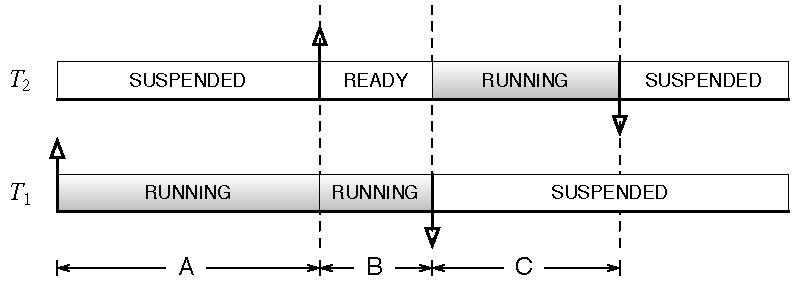
\includegraphics[scale=.7]{pictures/schedulingT1lp.pdf}
   \end{minipage}\hfill
   \begin{minipage}[c]{.3\linewidth}
   \begin{lstlisting}[language=C]
   TASK(T2) {
     ... /* C period */
     TerminateTask();
   }
   
   TASK(T1) {
     ... /* A period */
     ActivateTask(T2);
     ... /* B period */
     TerminateTask();
   }
 \end{lstlisting}
   \end{minipage}
   \caption{{\bfseries Activation of a lower priority task.} $Prio(T_1) \ge Prio(T_2)$. During A period, $T_1$ is {\sffamily\scshape running} and $T_2$ is {\sffamily\scshape suspended}. Then $T_1$ calls {\upshape\ttfamily ActivateTask(T2);}. Since $T_2$ does not have a higher priority, it becomes {\sffamily\scshape ready} (B period).  $T_1$ terminates and $T_2$ runs (C period) until it terminates.}
   \label{fig:scheduleT1lp}
\end{figure} 

\begin{figure}[htbp] %  figure placement: here, top, bottom, or page
   \centering
   \begin{minipage}[c]{.6\linewidth}
   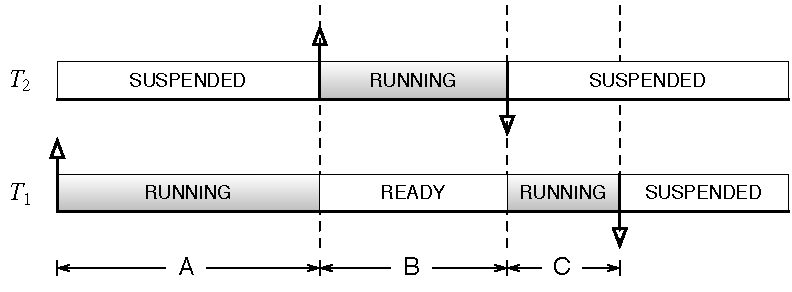
\includegraphics[scale=.7]{pictures/schedulingT1hp.pdf}
   \end{minipage}\hfill
   \begin{minipage}[c]{.3\linewidth}
   \begin{lstlisting}[language=C]
   TASK(T2) {
     ... /* B period */
     TerminateTask();
   }
   
   TASK(T1) {
     ... /* A period */
     ActivateTask(T2);
     ... /* C period */
     TerminateTask();
   }
 \end{lstlisting}
   \end{minipage}
   \caption{{\bfseries Activation of a higher priority task.} $Prio(T_1) < Prio(T_2)$. During A period, $T_1$ is {\sffamily\scshape running} and $T_2$ is {\sffamily\scshape suspended}. Then $T_1$ calls {\upshape\ttfamily ActivateTask(T2);}. Since $T_2$ has a higher priority, it becomes {\sffamily\scshape running} (B period).  $T_2$ terminates and $T_1$ resumes (C period) until it terminates.}
   \label{fig:scheduleT1hp}
\end{figure} 


\begin{figure}[htbp] %  figure placement: here, top, bottom, or page
   \centering
   \begin{minipage}[c]{.6\linewidth}
   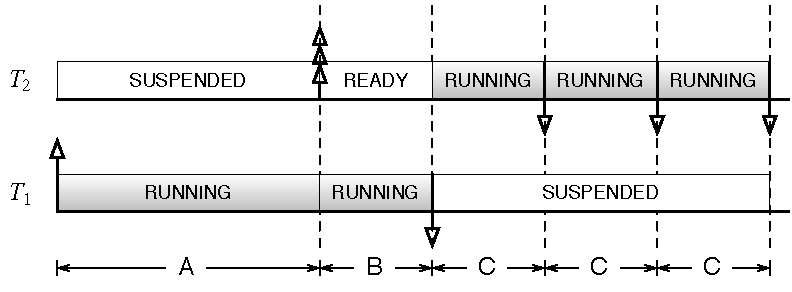
\includegraphics[scale=.7]{pictures/schedulingMultiple.pdf}
   \end{minipage}\hfill
   \begin{minipage}[c]{.3\linewidth}
   \begin{lstlisting}[language=C]
   TASK(T2) {
     ... /* C period */
     TerminateTask();
   }
   
   TASK(T1) {
     ... /* A period */
     ActivateTask(T2);
     ActivateTask(T2);
     ActivateTask(T2);
     ... /* B period */
     TerminateTask();
   }
 \end{lstlisting}
   \end{minipage}
   \caption{{\bfseries Multiple activations of a lower priority task.} $Prio(T_1) \ge Prio(T_2)$. During A period, $T_1$ is {\sffamily\scshape running} and $T_2$ is {\sffamily\scshape suspended}. Then $T_1$ calls {\upshape\ttfamily ActivateTask(T2);} 3 times. Since $T_1$ has a higher priority, $T_2$ does not run immediately and the 3 activations are recorded provided the ACTIVATION attribute in the OIL description of the task is a least 3 (B period). When $T_1$ terminates, the scheduler executes $T_2$ 3 times (C periods).}
   \label{fig:scheduleMultiple}
\end{figure} 



\begin{service}{ChainTask}{StatusType}

\note{This service does a rescheduling}

This service puts task TaskID in \READY\ state, and the calling task in the \SUSPENDED\ state. It acts as the \api{TerminateTask} service for the calling task.
\argument{TaskType}{TaskID}{The id of the task to activate}
\resultcode{\OK}{No error, the task TaskID has been successfully activated and the calling task has been successfully terminated. Note in this case {\ttfamily\servicename} does not return so actually \OK\ is never returned}
\resultcodeext{\OSID}{Invalid TaskID. No task with such an id exists}
\resultcode{\OSLIMIT}{Too many activations of the task}
\resultcodeext{\OSRESOURCE}{The calling task still held a resource}
\resultcodeext{\OSCALLLEVEL}{Called outside of a task}
\end{service}

\begin{figure}[htbp] %  figure placement: here, top, bottom, or page
   \centering
   \begin{minipage}[c]{.6\linewidth}
   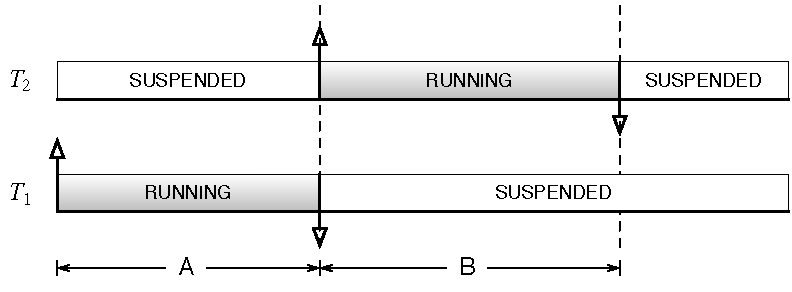
\includegraphics[scale=.7]{pictures/schedulingChain.pdf}
   \end{minipage}\hfill
   \begin{minipage}[c]{.3\linewidth}
   \begin{lstlisting}[language=C]
   TASK(T2) {
     ... /* B period */
     TerminateTask();
   }
   
   TASK(T1) {
     ... /* A period */
     ChainTask(T2);
   }
 \end{lstlisting}
   \end{minipage}
   \caption{{\bfseries Chaining of tasks.} During A period, $T_1$ is {\sffamily\scshape running} and $T_2$ is {\sffamily\scshape suspended}. Then $T_1$ calls {\upshape\ttfamily ChainTask(T2);}. $T_1$ terminates and $T_2$ is activated. Then $T_2$ runs (B periods).}
   \label{fig:scheduleMultiple}
\end{figure} 

\begin{service}{TerminateTask}{StatusType}

\note{This service does a rescheduling}

This service stops the calling task and puts it in \SUSPENDED\ state.
\resultcode{\OK}{No error, the calling task has been successfully terminated. Note in this case {\ttfamily\servicename} does not return so actually \OK\ is never returned}
\resultcodeext{\OSRESOURCE}{The calling task still held a resource}
\resultcodeext{\OSCALLLEVEL}{Called outside of a task}
\end{service}

\begin{service}{Schedule}{StatusType}
\note{This service does a rescheduling. 
Schedule does not deal directly with tasks but since it is a call to the scheduler, it is presented here.}

If called from a preemptable task that does not use an internal resource, Schedule has not effect. If called from a preemptable or a task that uses an internal resource, the priority of the task revert to its base priority and a rescheduling occurs.

Schedule allows to implement cooperative multitasking to insure synchronous rescheduling.
\resultcode{\OK}{No error.}
\resultcodeext{\OSRESOURCE}{The calling task still held a resource}
\resultcodeext{\OSCALLLEVEL}{Called outside of a task}
\end{service}

\begin{service}{GetTaskID}{StatusType}
\cfunction{\servicename} writes in the \var{TaskID} variable passed as reference the identifier of the task currently \RUNNING. If no task is currently \RUNNING\ because \cfunction{\servicename} was called from an ISR of before Trampoline is started, \constant{INVALID_TASK} is got.

\warning{The argument is a pointer. Do not pass an uninitialized pointer. Proper use of this service supposes a \ctype{TaskType} variable is instantiated, then its address is passed to \cfunction{\servicename} as shown in the example below:}

\begin{lstlisting}[language=C]
TaskType runningTaskID;
GetTaskID(&runningTaskID);
\end{lstlisting}

\resultcode{\OK}{No error.}
\resultcodeMP{\OSPROTECTIONMEMORY}{The caller does not have access to the addresses of \var{TaskID} reference} 
\argument{TaskRefType}{TaskID}{Reference to the task}
\end{service}

\begin{service}{GetTaskState}{StatusType}
\cfunction{\servicename} writes in the variable passed as reference in \var{State} the state of the task given in \var{TaskID}.

\warning{The \var{State} argument is a pointer. Do not pass an uninitialized pointer. Proper use of this service supposes a \ctype{TaskState} variable is instantiated, then its address is passed to \cfunction{\servicename} as shown in the example below:}

\begin{lstlisting}[language=C]
TaskStateType T1State;
GetTaskState(T1, &T1State);
\end{lstlisting}

\resultcode{\OK}{No error.}
\resultcodeext{\OSID}{Invalid TaskID. No task with such an id exists}
\resultcodeMP{\OSPROTECTIONMEMORY}{The caller does not have access to the addresses of \var{State} reference} 
\argument{TaskType}{TaskID}{The id of the task.}
\argument{TaskStateRefType}{State}{Reference to the state.}
\end{service}


%\strong{Processes} are both Tasks and ISRs category 2. Trampoline category 2 ISRs are like Basic Tasks except the priority level of the interrupt controller is raised to the priority of the ISR while the later is running.

\section{Inside Task management}
\label{sec:addtaskstate}

\subsection{Static attributes}

A task has the following static attributes:

\begin{description}
\item[The entry point of the task.] A pointer to the code of the task. When the scheduler start a task instance the first time, it uses this pointer to begin the execution.
\item[The internal resource] the task uses if any. An internal resource is automatically taken when a task enters the \RUNNING\ state and automatically released when the task leaves the \RUNNING\ state. See \ref{sec:internalresources} for more informations.
\item[The base priority] of the task as specified in the OIL file. This priority is used to reset the current priority when the task is activated.
\item[The maximum activation count] of the task as specified in the OIL file.
\item[The kind of task,] \BASIC\ or \EXTENDED.
\item[The task id.] Used for internal checking.
\item[The id of the OS Application] the tasks belong to (only available in \autosar\ \SC{3} and \SC{4}).
\item[The timing protection configuration] if any (only available in \autosar\ \SC{2} and \SC{4}).
\end{description}

\subsection{Dynamic attributes}

A task has also the following dynamic attributes:

\begin{description}
\item[The context.] This is the chunk of RAM where the current execution context of a task is stored when the task is in the \READY\ or \WAITING\ state. The execution context is the value of the microprocessor's registers (program counter, stack pointer, other working registers). So the context depends on the target on which Trampoline runs.
\item[The stack(s).] This is the chunk of RAM where registers are pushed for function call. This attributes depends on the target architecture. For instance, the C166 micro-controller uses 2 stacks.
\item[The current activation count.] When a task is activated while not in \SUSPENDED\ state, the activation is recorded and is actually done when the task returns to the \SUSPENDED\ state.  Many activation may be recorded according to the value given to the \oilattr{ACTIVATION} task OIL attribute. When a task is activated, the current activation count is compared to the maximum activation count and if $\ge$, the activation fails.
\item[The list of resources] the task currently owns.
\item[The current priority] of the task. This priority starts equal to the basic priority and may increase when the task get a resource.
\item[The state of the task] as defined in sections \ref{sec:taskstate} and \ref{sec:internaltaskstate}.
\item[The trusted counter.] If $=0$, the task is non-trusted. If $>0$ the task is trusted. See chapter \ref{chap:osapplications} for more informations. This counter is available if Trampoline is compiled with memory protection support.
\item[The activation allowed flag.] If true, the task may be activated. If false, it cannot be activated. This flag is set by the timing protection facility. It is available if Trampoline is compiled with timing protection support. See chapter \ref{chap:timingprotection}.
\end{description}

\subsection{Additional task states}
\label{sec:internaltaskstate}

In addition to states presented in section \ref{sec:taskstate}, 2 extra states are used for internal management: 

\begin{description}
\item[\AUTOSTART] This state is used to indicate what task should be started automatically when \api{StartOS} is called. An \AUTOSTART\ task is in this initial state but no task is in this state once the application code is running. \api{StartOS} iterates through the tasks and activates those that are in the \AUTOSTART\ state.
\item[\READYANDNEW] This state is used to flag a task that is ready but has its context uninitialized. This happens when the task has just been activated. The kernel initializes the context of the task the first time it goes to the \RUNNING\ state.
\end{description}

Figure \ref{fig:states} show a complete task state automaton for both basic and extended tasks with these states added.

\begin{figure}[htbp] %  figure placement: here, top, bottom, or page
   \centering
   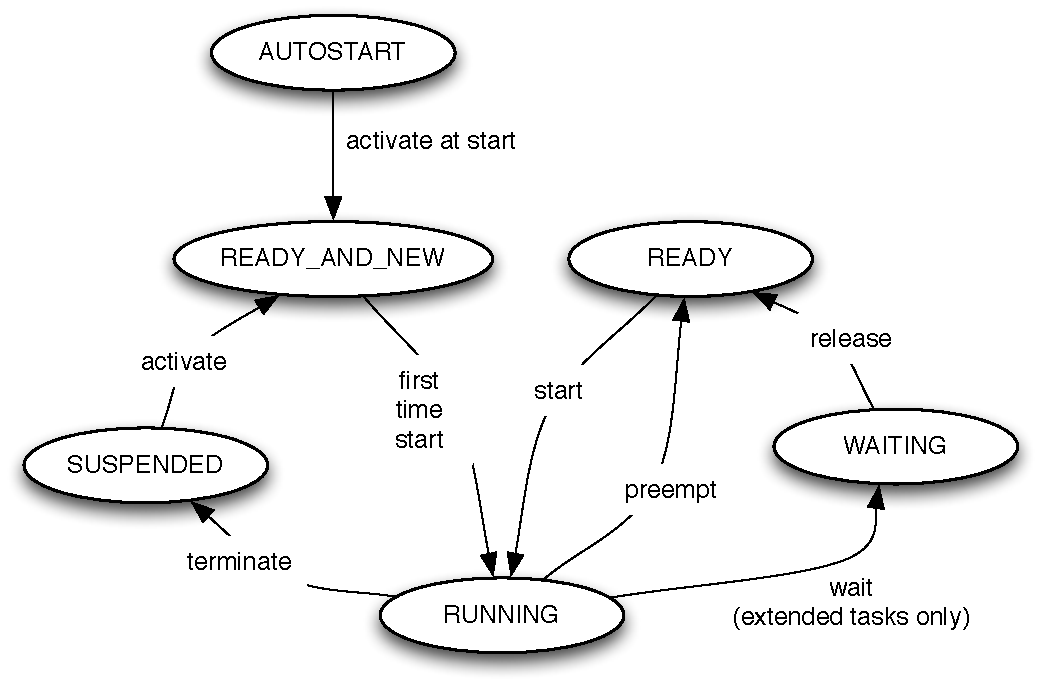
\includegraphics[width=4in]{pictures/states.pdf} 
   \caption{States of a task in Trampoline. \cmacro{AUTOSTART} is the initial state of autostart tasks. \cmacro{SUSPENDED} is the initial state of both non autostart tasks.}
   \label{fig:states}
\end{figure} 


\section{The {\em idle} task}

The {\em idle} task is activated by \api{StartOS}. It is a \BASIC\ task with a priority of 0 (\ie\ the lowest priority in the system, the lowest priority of tasks defined in the application is 1). So when no other task is currently running, the {\em idle} task run.

To be able to use specific platform capabilities (to put the micro-controller in stand by mode for example), this task calls repetitively a hardware specific function called \cfunction{tpl_sleep} (defined in \textit{machines/}). The tasks is then able to quantify the microprocessor occupation.

GOIL doesn't produce anything about this idle task (unlike application(s) task(s)). The idle task descriptor is defined in \file{tpl_os_kernel.c}.
%!TEX root = ./main.tex

\chapter{Alarms}
\label{chap:alarms}

\lettrine{A}larms are used to perform an action after an interval of time for a single shot alarm and periodically for a periodic alarm. The action may be the activation of a task, the setting of an event to a task or the execution of an alarm callback function\footnote{This third action is not available in AUTOSAR}.




% Activate the following line by filling in the right side. If for example the name of the root file is Main.tex, write
% "...root = Main.tex" if the chapter file is in the same directory, and "...root = ../Main.tex" if the chapter is in a subdirectory.
 
%!TEX root = main.tex

\chapter{Resources}
\label{chap:resources}

A resource is an object used to protect a critical section in a task or in an ISR and to insure mutual exclusion.
By using a resource to protect the use of a shared piece of data or a shared hardware device, the programmer avoids race conditions.
Figure \ref{fig:exampleRaceCondition} shows an example of race condition.


\begin{figure}[htbp] %  figure placement: here, top, bottom, or page
   \centering
   \begin{minipage}[c]{.55\linewidth}
\begin{lstlisting}[language=C]
int val = 0;
int actCount = 0;

TASK(bgTask)
{
  while (1) {
    val++;
    val--;
  }
}

TASK(periodicTask)
{

  activationCount++;
  if ((actCount % 2) == 1) {
    val++;
  }
  else {
    val--;
  }
    
  TerminateTask();
}

TASK(displayTask)
{
  printf("val=%d count=%d\n",
         val,
         activationCount);
    
  TerminateTask();
}
\end{lstlisting}
   \end{minipage}\hfill
   \begin{minipage}[c]{.35\linewidth}
\begin{lstlisting}[language=C]
val=2 count=10
val=3 count=20
val=4 count=30
val=5 count=40
val=2 count=50
val=2 count=60
val=0 count=70
val=-2 count=80
val=-1 count=90
val=-1 count=100
val=-2 count=110
val=0 count=120
val=0 count=130
val=0 count=140
val=0 count=150
val=-2 count=160
val=-1 count=170
val=-2 count=180
val=-4 count=190
val=-4 count=200
val=-6 count=210
val=-4 count=220
val=-5 count=230
val=-6 count=240
val=-7 count=250
val=-6 count=260
val=-3 count=270
val=-3 count=280
val=-5 count=290
val=-5 count=300
\end{lstlisting}
   \end{minipage}
   \caption{{\bfseries Shared data access.} In this example 3 preemptable tasks are used. \constant{bgTask} increments and decrements the global integer variable \var{shared} in an infinite loop. \constant{periodicTask} runs every 100ms and increments the global integer variable \var{activateCount}. If \var{activateCount} is odd, \constant{periodicTask} increments \var{shared} otherwise it is decremented. A third task, \constant{displayTask} runs every second and displays both variables. On the left, the corresponding program, on the right one of the possible outputs}
   \label{fig:exampleRaceCondition}
\end{figure}

\section{\osek\ Priority Ceiling Protocol}

\osek\ uses a modified version of the Priority Ceiling Protocol\,\cite{PCP}. A priority is assigned to each resource. This 
priority is computed to be at least equal to the highest priority of the tasks and ISRs that use the resource. So let $T_1, T_2, \dots, T_n$ a set of tasks sharing the same resource $R$ and $P_1, P_2, \dots, P_n$ their priorities so that $P_i = P(T_i)$. We have $P(R) = \max_{i=1,n}(P_i)$.

When a task gets a resource, its priority is raised to the priority of the resource. That way, the task will run with the priority of the highest priority task and will insure the release of the resource is not delayed by a lower priority task. In addition, since every other tasks that use the same resource have now a priority $\leq$, they cannot preempt the running task and mutual exclusion is insured. Figure \ref{fig:exampleResource} show an example of resource use.

\begin{figure}[htbp] %  figure placement: here, top, bottom, or page
   \centering
   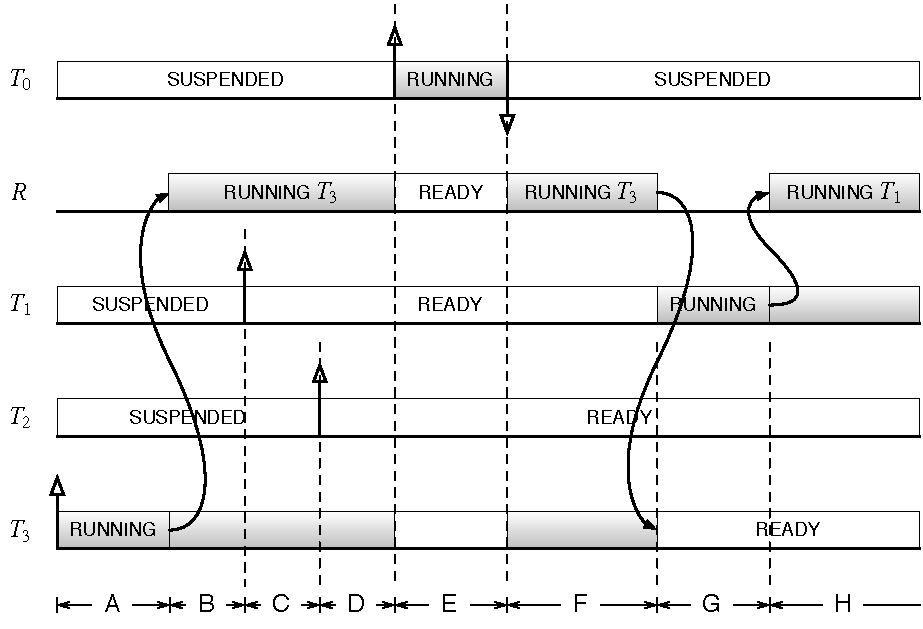
\includegraphics[scale=.7]{pictures/schedulingResource.pdf} 
   \caption{{\bfseries Scheduling with a resource used by 3 tasks and a fourth task having a higher priority.} $P(T_0)>P(T_1)>P(T_2)>P(T_3)$. $R$ is used by $T_1$, $T_2$ and $T_3$ so $P(T_0)>P(R)\ge P(T_1)$. During A period, $T_3$ is {\sffamily\scshape running} and other tasks are {\sffamily\scshape suspended}. Then $T_3$ gets $R$ and $P(T_3) \leftarrow P(R)$ (B to F periods). $T_1$ is activated and becomes {\sffamily\scshape ready}; since $P(T_3) \ge P(T_1)$, $T_1$ does not run (C to F periods). $T_2$ is activated and becomes {\sffamily\scshape ready}; for the same reason it does not run (D to H periods). $T_0$ is activated and because $P(T_0)>P(R)$ it runs (E period). $T_0$ terminates and $T_3$ continues its execution (F period). Then $T_3$ releases $R$ and $P(T_3)$ reverts to its base priority; so since $P(T_1)>P(T_2)>P(T_3)$, $T_1$ runs (G period). $T_1$ gets $R$ and $P(T_1) \leftarrow P(R)$ (H period).}
   \label{fig:exampleResource}
\end{figure} 

The priority of a resource is computed by \goil\ according to the priorities of the tasks and ISRs that use the resource.

\section{The {\ttfamily RES_SCHEDULER} resource}

Trampoline provides a predefined standard resource called \constant{RES_SCHEDULER}. This resource has a priority $\ge$ to the maximum priority of the tasks but $<$ to the minimum priority of the ISR. When a task gets \constant{RES_SCHEDULER}, it becomes non preemptable. To make \constant{RES_SCHEDULER} available to the application, the \oilattr{USERESCHEDULER} attribute must be set to \TRUE\ within the \oilattr{OS} object in the OIL file. Unlike resources defined by the application, there is no need to declare \constant{RES_SCHEDULER} is used by a task in the OIL file.

\section{Standard and Internal Resources}

Standard resources are got and released explicitly by tasks and ISRs using the ad-hoc services. Internal resources are got implicitly when the task enters the \RUNNING\ state and released implicitly when the task calls \api{Schedule} or blocks when using \api{WaitEvent}.

Standard resources are dedicated to the protection of critical sections around the access to a shared data or to a device. Internal resources are used to implement non preemptable tasks within a task group.
A task group is a set of task that are non preemptable by each other but remain preemptable by higher priority tasks in the application. A task group priority is the priority of its internal resource.

Trampoline provides a predefined internal \constant{RES_SCHEDULER} resource with the same priority. This internal resource is used to implement non preemptable tasks in the whole application as if all the non preemptable tasks belong to an implicit task group. When a task is non preemptable by setting the \oilattr{SCHEDULE} attribute to \constant{NON} in its OIL description, the task is assigned the internal \constant{RES_SCHEDULER} resource.

\section{OIL description}

A resource is described using a \oilattr{RESOURCE} object. \oilattr{RESOURCEPROPERTY} is the single attribute of this object. A standard resource is defined with the following code:

\begin{lstlisting}[language=OIL]
RESOURCE res {
  RESOURCEPROPERTY = STANDARD;
};
\end{lstlisting}

And an internal resource is defined with the following code:

\begin{lstlisting}[language=OIL]
RESOURCE other_res {
  RESOURCEPROPERTY = INTERNAL;
};
\end{lstlisting}

A third kind of declaration exists for {\bfseries\oilattr{LINKED}} resources. A linked resource may be linked to a linked resource or a standard resource but a link tree of resources must have a standard resource at the root. A linked resource has the same priority as the standard resource it is linked to and is a kind of reference. Linked resources are provided to replace nested access to the same resource (which is prohibited) and are rarely used.

\begin{lstlisting}[language=OIL]
RESOURCE l_res {
  RESOURCEPROPERTY = LINKED { LINKEDRESOURCE = res };
};
\end{lstlisting}


\begin{service}{SetEvent}{StatusType}
Events of task TaskID are set according to the Mask passed as 2nd argument. This service is non blocking and may be called from a task or an ISR2
\argument{TaskType}{TaskID}{the id of the task}
\argument{EventMaskType}{Mask}{the event mask}
\resultcode{\OK}{No error}
\resultcodeext{\OSID}{Invalid TaskID}
%E_OS_ACCESS: TaskID is not an extended task (not able to manage events);
%E_OS_STATE: Events cannot be set because the target task is in the SUSPENDED state.
\end{service}

%!TEX root = ./trampoline.tex

\chapter{OS Applications}

OS Applications are a set of objects managed by Trampoline and sharing common data and access rights.

\section{Execution of the OS Applications startup and shutdown hooks}

These hooks are executed from the kernel but with the access right of a task belonging to the OS Application. The \sysgen\ should choose one of the tasks of the OS Application to be used as context to execute the OS Application startup and shutdown hooks. Execution of an OS Application startup hook is done by the \cfunction{tpl_call_startup_hook_and_resume} function. The argument of this function is a function pointer to the hook. Similarly execution of an OS Application shutdown hook is done by the \cfunction{tpl_call_shutdown_hook_and_resume} function. These functions end by a call to \api{NextStartupHook} and \api{NextShutdownHook} services respectively to cycle through the hooks.

%!TEX root = ./trampoline.tex

\chapter{Timing Protection Implementation}

The Timing Protection Implementation uses 2 timers. The first one is a {\em Free Running Timer} (FRT) which is used for {\em Time Frame}. The second one is a classical timer called {\em Timing Protection Timer} (TPT) which is used for \emph{Execution Time Budget}, \emph{Resource Locking Budget} and \emph{Interrupt Disabling Budget}.

\section{Low Level Functions}

These functions are provided by the {\em Board Support Package} and are used to manage the timers needed by the Timing Protection.

\subsection{FRT related functions}

\paragraph{\function{tpl_status tpl_start_frt(void)}} starts the FRT. On a microcontroller having a FRT that starts automatically when the system is powered on, this function does nothing but must be present since it is called by Trampoline in initialization stage. An error code is returned: {\em E\_OK} means no error, {\em E\_OS\_NOFUNC} means the FRT could not be started.

\paragraph{\function{tpl_status tpl_read_frt(tpl_tp_tick *out_value)}} write the current value of the FRT in \var{out_value}. An error code is returned: {\em E\_OK} means no error, {\em E\_OS\_NOFUNC} means the FRT could not be read.

\paragraph{\function{tpl_status tpl_elapsed_frt(tpl_tp_tick last_tick, tpl_tp_tick *out_value)}} write the number of ticks elapsed since \var{last_tick} in \var{out_value}. If the FRT has overflown/underflown between the time \var{last_tick} was get and the time \function{tpl_elapsed_frt} is called, \function{tpl_elapsed_frt} gives a correct value. An error code is returned: {\em E\_OK} means no error, {\em E\_OS\_NOFUNC} means the FRT could not be read.

\subsection{TPT related functions}

\paragraph{\function{tpl_status tpl_init_tpt(???)}} initializes the TPT. An error code is returned: {\em E\_OK} means no error, {\em E\_OS\_NOFUNC} means the TPT could not be initialized.

\paragraph{\function{tpl_status tpl_deinit_tpt(void)}} deinitializes the TPT. An error code is returned: {\em E\_OK} means no error, {\em E\_OS\_NOFUNC} means the TPT could not be deinitialized.

\paragraph{\function{tpl_status tpl_start_tpt(tpl_tp_tick delay)}} starts the TPT with an expiration delay equal to \var{delay} ticks. At that time, the \function{tpl_tpt_handler} function is called. An error code is returned: {\em E\_OK} means no error, {\em E\_OS\_NOFUNC} means the TPT could not be started because it is not initialized.

\paragraph{\function{tpl_status tpl_read_tpt(tpl_tp_tick *out_value)}} write the current value of the TPT in \var{out_value}. An error code is returned: {\em E\_OK} means no error, {\em E\_OS\_NOFUNC} means the TPT could not be read.

\paragraph{\function{tpl_status tpl_elapsed_tpt(tpl_tp_tick last_tick, tpl_tp_tick *out_value)}} write the number of ticks elapsed since \var{last_tick} in \var{out_value}. An error code is returned: {\em E\_OK} means no error, {\em E\_OS\_NOFUNC} means the TPT could not be read.




%% HEAD SUPERTABULAR %%
\rowcolors{1}{light-gray}{white}
\newlength{\Li}\settowidth{\Li}{\textbf{Decimal}}
\newlength{\Liii}\settowidth{\Liii}{(bootstrap  )}
\newlength{\Lii}\settowidth{\Lii}{SCHEDULETABLE\_AUTOSTART }
\tablefirsthead{ \textbf{Decimal Value} & \textbf{bit 5}  & \textbf{bit 4} & \textbf{bit 3} & \textbf{bit 2} & \textbf{bit 1} & \textbf{bit 0} & \textbf{Meaning} \\ \hline }
\tablehead{ \rowcolor{white} \rowcolors{1}{light-gray}{white} \textbf{Decimal Value} & \textbf{bit 5}  & \textbf{bit 4} & \textbf{bit 3} & \textbf{bit 2} & \textbf{bit 1} & \textbf{bit 0} & \textbf{Meaning} \\ \hline  }
\tabletail{ \hline } 
\tablelasttail{}


\chapter{Schedule Table Implementation}

\section{The States of a Schedule Table}

A schedule table always has a defined state. States include those found at page 42 of the AUTOSAR specifications 3.1 and others states used for internal management.

Indeed, \textbf{bit 1} is the "autostart" bit. It's used when autostarted schedule tables have been declared in the OIL file. Goil generates schedule tables with SCHEDULETABLE\_AUTOSTART\_X (X can be RELATIVE, ABSOLUTE or SYNCHRON) state. At startup (in tpl\_init\_os()), the system starts autostarted schedule tables and resets the \textbf{bit 1}.

\textbf{bit 4} is the "bootstrap" bit. It's used when the first expiry point of a schedule table is dated in more than \textbf{OsCounterMaxAllowedValue} ticks from the current date \footnote{As the \textit{$<$offset$>$} parameter of StartScheduleTableRel() cannot be greater than \textbf{OsCounterMaxAllowedValue} minus the \textbf{InitialOffset} of the schedule table (OS276), the first expiry point cannot be in more than \textbf{OsCounterMaxAllowedValue} ticks from the current date. Thus the "bootstrap" bit can set by StartScheduleTableAbs() only.}. It can happen when :
	\begin{itemize}
	\item the schedule table start ($<$tick\_val$>$) is after the current date and the first expiry point comes between the current date and $<$tick\_val$>$
	\item $<$tick\_val$>$ is before the current date and the first expiry point comes after the current date
	\end{itemize}

The \textbf{bit 5} is the "asynchronous" bit. It tells the system that the schedule table is in asynchronous mode.\\

\begin{center}
\topcaption{\textcolor{white}{q}States of a schedule table } % Latex is weird, the table goes on the next page without the "\textcolor{white}{q}"
\begin{supertabular}{p{\Li}|c|c|c|c|c|c|p{\Lii}|} 
0	& 0	& 0	& 0 	& 0	& 0	& 0	& SCHEDULETABLE\_STOPPED  \\ 
1	& 0	& 0	& 0 	& 0	& 0	& 1	& SCHEDULETABLE\_RUNNING  \\ 
5	& 0	& 0	& 0 	& 1	& 0	& 1	& SCHEDULETABLE\_NEXT  \\  
9	& 0	& 0	& 1 	& 0	& 0	& 1	& SCHEDULETABLE\_WAITING  \\  
13	& 0	& 0	& 1 	& 1	& 0	& 1	& SCHEDULETABLE\_RUNNING\_AND\_SYNCHRONOUS \\ %\hline \hline
6	& 0	& 0	& 0 	& 1	& 1	& 0	& SCHEDULETABLE\_AUTOSTART \_ABSOLUTE  \\ 
10	& 0	& 0	& 1 	& 0	& 1	& 0	& SCHEDULETABLE\_AUTOSTART \_RELATIVE  \\  
14	& 0	& 0	& 1 	& 1	& 1	& 0	& SCHEDULETABLE\_AUTOSTART \_SYNCHRON  \\  \hline \hline
16	& 0	& 1	& 0 	& 0	& 0	& 0	& SCHEDULETABLE\_BOOTSTRAP \\ 
32	& 1	& 0	& 0 	& 0	& 0	& 0	& SCHEDULETABLE\_ASYNC  \\ 
\end{supertabular} 
\end{center}
\label{schedtablestates}

Figure  \ref{fig:STstates} shows how a schedule table goes from state to state.

\begin{figure}[htbp] %  figure placement: here, top, bottom, or page
   \centering
   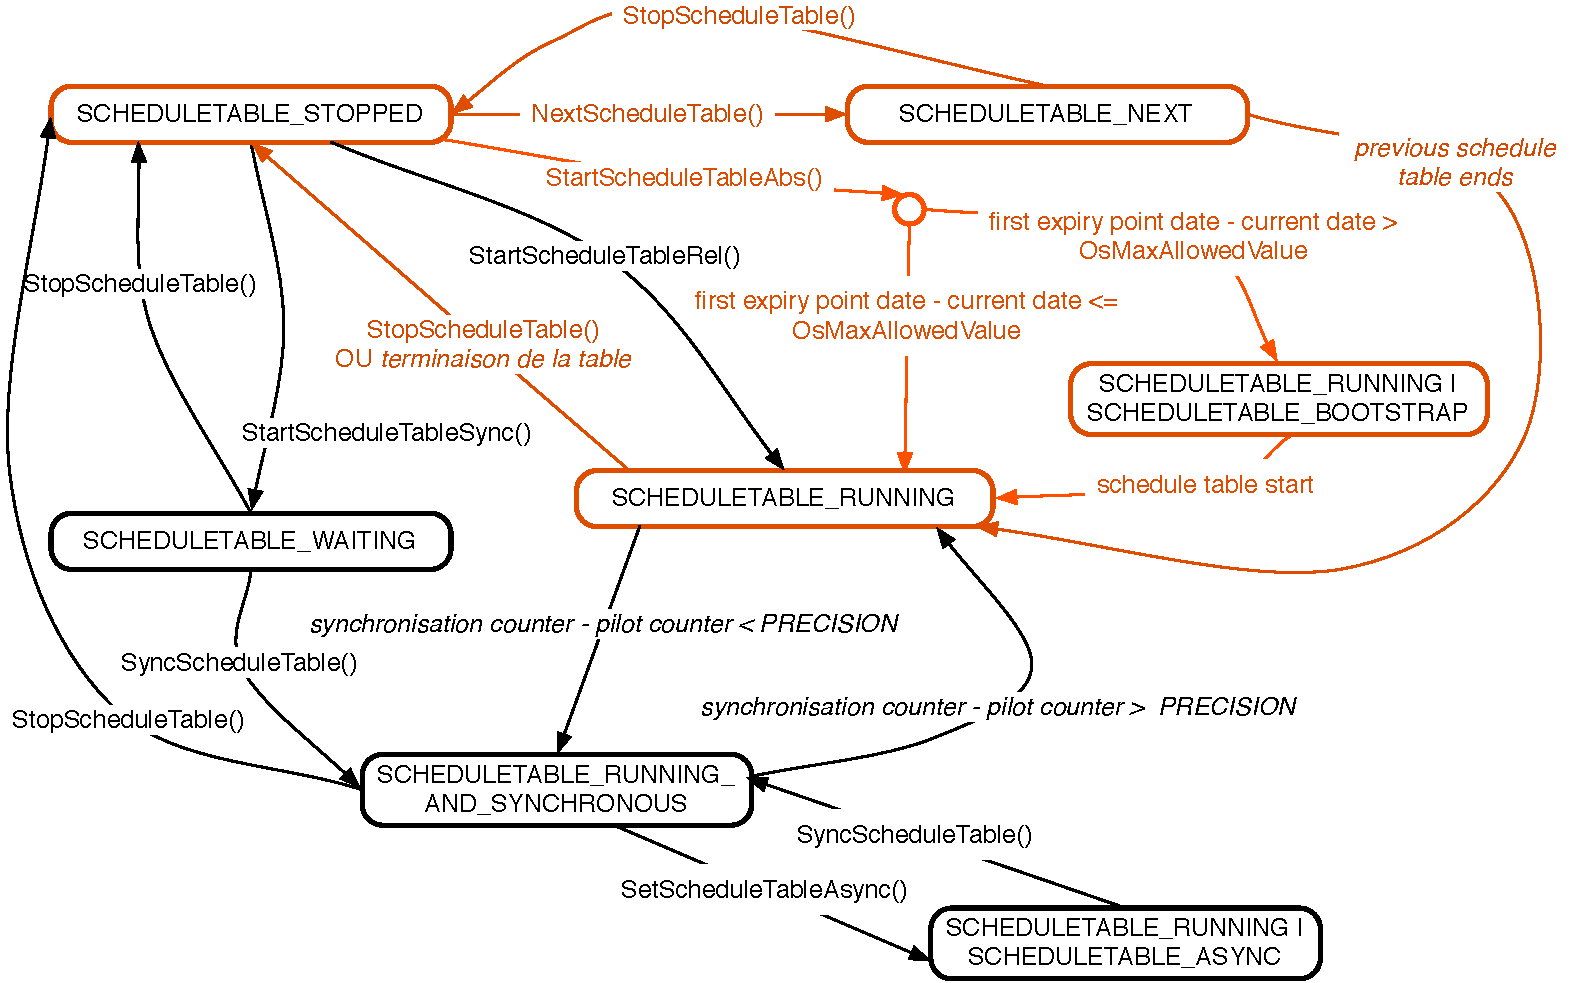
\includegraphics[width=6in]{pictures/STstates.pdf}  
   \caption{States of a schedule table in Trampoline.}
   \label{fig:STstates}
\end{figure} 
	
\section{Processing a Schedule Table}

Depending on the OIL file, GOIL generates one expiry point more than the number of expiry point delared by the User : the "finalize" expiry point. Indeed, the RUNNING state of a NEXT schedule table should be set at the finalize expiry point, thus, we have to add this expiry point to do it. For a periodic schedule table, the finalize expiry point helps to launch the first expiry point of the next period. The Figure below shows the processing schedule table petri net. \\%different expiry point actions and the one we've added for the finalize expiry point.

As a schedule table is a time object, as an alarm, ...\\

%figure showing that the tpl_process_schedtable() is the main function (launched by each expiry point of a schedule table). It increment the index of the expiry point, launch the action of the  index is incremented






























%!TEX root = ./trampoline.tex

\chapter{The communication library}

\section{Internals}


%!TEX root = ./main.tex

\chapter{The Inter OS-application Communication Library}

\lettrine{I}nter OS-application Communication library is an API initially dedicated to communications between tasks from different OS-applications in multicore systems. However, it could also be used for communications between tasks from a same OS-Application. In the fallowing, Inter OS-application Communication will be denoted IOC.
This chapter presents the IOC configuration and API.
Implementation details as well as examples of utilization are provided.

\section{IOC declaration in OIL}

The IOC configuration is performed using OIL. Parameters such as IOC name, the type of manipulated data, the kind of communication (queued or last is best) and informations about sender/receiver are mandatory. The syntax is presented below using tow example.

Let us consider the case where a task A (as part of OS-application \textit{os-app1}) sends a data to a task B (as part of OS-application \textit{os-app2}). 
In the first case, we consider a last is best semantic communication where only one data of type u8 is sent.
In the second case, we consider a queued semantic communication where a data of type u8 and a data of type \textit{mytype} (defined by user) are sent. It is worth noting that this type have to be defined by user un the file \textit{ioc_types.h} at the root of the project directory.

\textit{mytype} can be defined like this:

\begin{lstlisting}[language=C]
struct mytype {
  u8	  a;
  u8	  b,
}
\end{lstlisting}

\begin{lstlisting}[language=OIL]

/* LAST_IS_BEST semantic */

IOC com_A_to_B_last_is_best {
  DATATYPENAME u8 {
    DATATYPEPROPERTY = DATA;
  };
  SEMANTICS = LAST_IS_BEST {
    INIT_VALUE_SYMBOL = AUTO;
  };
  RECEIVER rcv {
    RCV_OSAPPLICATION = os-app2;
    RECEIVER_PULL_CB = AUTO;
    ACTION = NONE;
  };
  SENDER sender0 {
    SENDER_ID = 0;
    SND_OSAPPLICATION = os-app1;
  };
}; 

/* QUEUED semantic */

IOC com_A_to_B_queued {
  DATATYPENAME u8 {
    DATATYPEPROPERTY = DATA;
  };
  DATATYPENAME mytype {
    DATATYPEPROPERTY = REFERENCE;
  };
  SEMANTICS = QUEUED {
    BUFFER_LENGTH = 2;
  };
  RECEIVER rcv {
    RCV_OSAPPLICATION = os-app2;
    RECEIVER_PULL_CB = AUTO;
    ACTION = NONE;
  };
  SENDER sender0 {
    SENDER_ID = 0;
    SND_OSAPPLICATION = os-app1;
  };
}; 

\end{lstlisting}

The DATATYPENAME parameter defines the name of the data type to be transferred. A file named \textit{ioc_types.h} should be created by user in order to defined new types, if any. The associated property specifies if the data is passed to sending functions by reference or by value. It is worth noting that it is possible to specify many DATATYPENAME as illustrated with the second example. In that case, the applicative sending function should have as many parameters as the number of DATATYPE specify in the OIL file. 
In case of a last is best semantic, the INIT_VALUE_SUMBOL defines the initial data value. It can be set to AUTO is there are no initial value. Otherwise, the INIT_VALUE_SYMBOL is a string type defined by user and the function \textit{IOC_init()} has to be called at the beginning of application. In case of a queued semantic, only a BUFFER_LENGTH has to be specified.
The receiver configuration requires the setting of the target OS-application (RCV_OSAPPLICATION), the king of task notification used when the message has arrived (ACTION = ACTIVATETASK, SETEVENT or NONE) (not functional at the moment) and the callback function to call (not functional at the moment).
The sender configuration require the SENDER_ID, as an integer, and the sender OS-application (SND_OSAPPLICATION). 

\section{Implementation}

The IOC is divided in two set of source files. First, the APIs (part of the OS) containing kernel functions are generic. They can be found in \textit{ioc/} directory. Second, specific files for the IOC configuration are generated. The IOC API is very closed to internal communication library and will not be detailed here. Let us now detailed what is generated in \textit{tpl_ioc_api_config.c}.

In case of the last is best communication (example 1), the sending operation is performed by the call of \textit{IocWrite_IocName()} function and the receiving operation, by the call of the function \textit{IocRead_IocName()}. These functions have to be called directly by user in applicative functions. The generated part of the API transmit the request to the kernel. Let us now illustrated the generated code for the first example.

\begin{lstlisting}[language=C]

FUNC(Std_ReturnType, OS_CODE) IocWrite_com_A_to_B_last_is_best(
  VAR(u8, AUTOMATIC) IN0 /* one data is send */
)
{
  /* only one data implies only one element in the message table */
  VAR(tpl_ioc_message, AUTOMATIC) message[1]; 
  VAR(Std_ReturnType, AUTOMATIC) result;

  /* Fill in the message structure with the data address and its size */
  message[0].data=(tpl_ioc_data *)&IN0;
  message[0].length=sizeof(u8);
  
  /* Call the kernel function */
  result = IOC_Write(0, message); 
  
  return result;
}

FUNC(Std_ReturnType, OS_CODE) IocRead_com_A_to_B_last_is_best(
  P2VAR(u8, AUTOMATIC, OS_APPL_DATA) IN0
)
{
  VAR(tpl_ioc_message, AUTOMATIC) message[1];
  VAR(Std_ReturnType, AUTOMATIC) result;

  message[0].data=(tpl_ioc_data *)IN0;
  message[0].length=sizeof(u8);
  
  /* Call the kernel function */
  result = IOC_Read(0, message);
  
  return result;
}

\end{lstlisting}


In the case of a queued communication, the sending and receiving operations are performed by the call of \textit{IocSend_IocName()} and \textit{IocReceive_IocName()} respectively. Generated functions would be of the same form that in last is best case.

Finally, it is possible that several senders send a same data. In that case, many senders can be defined during the OIL configuration. In the applicative functions, user have to call API functions of type \textit{IocWrite_IocName_SenderName() or IocSend_IocName_SenderName()} when sending a message.
%!TEX encoding = UTF-8 Unicode
%!TEX root = ./main.tex

\chapter{Memory mapping}

\lettrine{T}he \autosar\ consortium has defined a set of macros\,\cite{autosar44CompilerAbstraction} in order to adapt the memory mapping directives to the different existing compilers. Indeed, memory mapping directives are not part of the C language and it is therefore impossible to write portable code between different compilers without going through this set of macros. In addition, some MCUs have a segmented memory model and require additional pointer directives to specify whether the pointer is to data in the same segment or to data in a different segment. In the first case, it is a \emph{near} pointer (usually stored in a 16 bits word). In the second case it is a \emph{far} pointer (usually stored in a 24 bits word).

It remains that these macros are not particularly intuitive in their use and require some explanations that we will give here.

\section{Memory mapping directives}

Memory mapping consists in assigning to each object of the application (variables, constants, functions) and of the operating system a named memory area where the object will be stored. Memory mapping directives take various forms depending on the compiler. For example, putting a function named \cfunction{f} in the memory area \ctype{.osCode} when using \tool{gcc} is done as follows:

\begin{lstlisting}[language=C]
void __attribute__ ((section (".osCode"))) f() { ... }
\end{lstlisting}

while doing the same thing using Freescale's CodeWarrior compiler (previously Metrowerks) requires the following directive:

\begin{lstlisting}[language=C]
#pragma section code_type ".osCode"
void f() { ... }
\end{lstlisting}

\autosar\ defines several macros to encapsulate these directives and these macros work with the declarations of the memory sections.

\section{The memory sections}

For each task and ISR declared in the OIL file, Goil generates several memory sections. These sections are selected via macro definitions with names of the form \cmacro{APP_Task_<name>_START_SEC_<section_type>} and \cmacro{APP_Task_<name>_STOP_SEC_<section_type>} for tasks and \cmacro{APP_ISR_<name>_START_SEC_<section_type>} and \cmacro{APP_ISR_<name>_STOP_SEC_<section_type>} for ISRs. \cmacro{<name>} is the name of the task or ISR and \cmacro{<section_type>} is the type of section. The section types are as follows:

\begin{description}

\item[\cmacro{CODE}] is the section used for the process code and for the functions called by the process. If, for example, the task t1 is declared in the OIL file, its code will be written in C as follows:
\begin{lstlisting}[language=C]
#define APP_Task_t1_START_SEC_CODE
#include "MemMap.h"
TASK(t1)
{
  ...
  TerminateTask();
}
#define APP_Task_t1_STOP_SEC_CODE
#include "MemMap.h"
\end{lstlisting}

\item[\cmacro{STACK}] is the section used for the process stack. This section is used in the files generated by \goil.

\item[\cmacro{VAR_<init_policy>_<alignment>}] are the sections used for process globals or static variables. \cmacro{<init_policy>} can take the following values:
  \begin{description}
  \item[\cmacro{NOINIT}] for uninitialized variables.
  \item[\cmacro{POWER_ON_INIT}] for variables initialized at MCU startup.
  \end{description}
\cmacro{<alignment>} can take the following values:
  \begin{description}
  \item[\cmacro{32BIT}] for 4 bytes alignment.
  \item[\cmacro{16BIT}] for 2 bytes alignment.
  \item[\cmacro{8BIT}] for 1 byte alignment.
  \item[\cmacro{UNSPECIFIED}] for data sizes that do not fit into any of the other categories.
  \end{description}

\item[\cmacro{CONST_<alignment>}] are the sections used for process globals constants.
\end{description}

For example, if task t1 uses two 8-bit constants, \var{c1} and \var{c2}, and one 32-bit variable, \var{v1}, uninitialized, they will be declared as follows:

\begin{lstlisting}[language=C]
#define APP_Task_t1_START_SEC_CONST_8BIT
#include "MemMap.h"
CONST(uint8, AUTOMATIC) c1 = 3;
CONST(uint8, AUTOMATIC) c2 = 7;
#define APP_Task_t1_STOP_SEC_CONST_8BIT
#include "MemMap.h"

#define APP_Task_t1_START_SEC_VAR_NOINIT_32BIT
#include "MemMap.h"
VAR(uint8, AUTOMATIC) v1;
#define APP_Task_t1_STOP_SEC_VAR_NOINIT_32BIT
#include "MemMap.h"
\end{lstlisting}



\begin{table}[htp]
\caption{Sections generated for task t1}
\begin{center}\scriptsize
\begin{tabular}{|c|c|}
\hline
APP_Task_toto_START_SEC_CODE & APP_Task_toto_STOP_SEC_CODE \\
APP_Task_toto_START_SEC_STACK & APP_Task_toto_STOP_SEC_STACK \\
APP_Task_toto_START_SEC_VAR_NOINIT_32BIT & APP_Task_toto_STOP_SEC_VAR_NOINIT_32BIT \\
APP_Task_toto_START_SEC_VAR_NOINIT_16BIT & APP_Task_toto_STOP_SEC_VAR_NOINIT_16BIT \\
APP_Task_toto_START_SEC_VAR_NOINIT_8BIT & APP_Task_toto_STOP_SEC_VAR_NOINIT_8BIT \\
APP_Task_toto_START_SEC_VAR_NOINIT_BOOLEAN & APP_Task_toto_STOP_SEC_VAR_NOINIT_BOOLEAN \\
APP_Task_toto_START_SEC_VAR_NOINIT_UNSPECIFIED & APP_Task_toto_STOP_SEC_VAR_NOINIT_UNSPECIFIED \\
APP_Task_toto_START_SEC_VAR_POWER_ON_INIT_32BIT & APP_Task_toto_STOP_SEC_VAR_POWER_ON_INIT_32BIT \\
APP_Task_toto_START_SEC_VAR_POWER_ON_INIT_16BIT & APP_Task_toto_STOP_SEC_VAR_POWER_ON_INIT_16BIT \\
APP_Task_toto_START_SEC_VAR_POWER_ON_INIT_8BIT & APP_Task_toto_STOP_SEC_VAR_POWER_ON_INIT_8BIT \\
APP_Task_toto_START_SEC_VAR_POWER_ON_INIT_BOOLEAN & APP_Task_toto_STOP_SEC_VAR_POWER_ON_INIT_BOOLEAN \\
APP_Task_toto_START_SEC_VAR_POWER_ON_INIT_UNSPECIFIED & APP_Task_toto_STOP_SEC_VAR_POWER_ON_INIT_UNSPECIFIED \\
APP_Task_toto_START_SEC_VAR_FAST_32BIT & APP_Task_toto_STOP_SEC_VAR_FAST_32BIT \\
APP_Task_toto_START_SEC_VAR_FAST_16BIT & APP_Task_toto_STOP_SEC_VAR_FAST_16BIT \\
APP_Task_toto_START_SEC_VAR_FAST_8BIT & APP_Task_toto_STOP_SEC_VAR_FAST_8BIT \\
APP_Task_toto_START_SEC_VAR_FAST_BOOLEAN & APP_Task_toto_STOP_SEC_VAR_FAST_BOOLEAN \\
APP_Task_toto_START_SEC_VAR_FAST_UNSPECIFIED & APP_Task_toto_STOP_SEC_VAR_FAST_UNSPECIFIED \\
APP_Task_toto_START_SEC_VAR_32BIT & APP_Task_toto_STOP_SEC_VAR_32BIT \\
APP_Task_toto_START_SEC_VAR_16BIT & APP_Task_toto_STOP_SEC_VAR_16BIT \\
APP_Task_toto_START_SEC_VAR_8BIT & APP_Task_toto_STOP_SEC_VAR_8BIT \\
APP_Task_toto_START_SEC_VAR_BOOLEAN & APP_Task_toto_STOP_SEC_VAR_BOOLEAN \\
APP_Task_toto_START_SEC_VAR_UNSPECIFIED & APP_Task_toto_STOP_SEC_VAR_UNSPECIFIED \\
APP_Task_toto_START_SEC_CONST_32BIT & APP_Task_toto_STOP_SEC_CONST_32BIT \\
APP_Task_toto_START_SEC_CONST_16BIT & APP_Task_toto_STOP_SEC_CONST_16BIT \\
APP_Task_toto_START_SEC_CONST_8BIT & APP_Task_toto_STOP_SEC_CONST_8BIT \\
APP_Task_toto_START_SEC_CONST_BOOLEAN & APP_Task_toto_STOP_SEC_CONST_BOOLEAN \\
APP_Task_toto_START_SEC_CONST_UNSPECIFIED & APP_Task_toto_STOP_SEC_CONST_UNSPECIFIED \\
APP_Task_toto_START_SEC_CALIB_32BIT & APP_Task_toto_STOP_SEC_CALIB_32BIT \\
APP_Task_toto_START_SEC_CALIB_16BIT & APP_Task_toto_STOP_SEC_CALIB_16BIT \\
APP_Task_toto_START_SEC_CALIB_8BIT & APP_Task_toto_STOP_SEC_CALIB_8BIT \\
APP_Task_toto_START_SEC_CALIB_BOOLEAN & APP_Task_toto_STOP_SEC_CALIB_BOOLEAN \\
APP_Task_toto_START_SEC_CALIB_UNSPECIFIED & APP_Task_toto_STOP_SEC_CALIB_UNSPECIFIED \\
APP_Task_toto_START_SEC_CARTO_32BIT & APP_Task_toto_STOP_SEC_CARTO_32BIT \\
APP_Task_toto_START_SEC_CARTO_16BIT & APP_Task_toto_STOP_SEC_CARTO_16BIT \\
APP_Task_toto_START_SEC_CARTO_8BIT & APP_Task_toto_STOP_SEC_CARTO_8BIT \\
APP_Task_toto_START_SEC_CARTO_BOOLEAN & APP_Task_toto_STOP_SEC_CARTO_BOOLEAN \\
APP_Task_toto_START_SEC_CARTO_UNSPECIFIED & APP_Task_toto_STOP_SEC_CARTO_UNSPECIFIED \\
APP_Task_toto_START_SEC_CONFIG_DATA_32BIT & APP_Task_toto_STOP_SEC_CONFIG_DATA_32BIT \\
APP_Task_toto_START_SEC_CONFIG_DATA_16BIT & APP_Task_toto_STOP_SEC_CONFIG_DATA_16BIT \\
APP_Task_toto_START_SEC_CONFIG_DATA_8BIT & APP_Task_toto_STOP_SEC_CONFIG_DATA_8BIT \\
APP_Task_toto_START_SEC_CONFIG_DATA_BOOLEAN & APP_Task_toto_STOP_SEC_CONFIG_DATA_BOOLEAN \\
\end{tabular}
\end{center}
\label{tab:memsections}
\end{table}%

%!TEX root = ./main.tex

\chapter{System generation and compilation}

\lettrine{T}rampoline is a static operating system. This means all the objects (tasks, ISR, ...) are known at compile time. This way, an application is made of tasks' code and ISRs' code, application data, and statically initialized descriptor for each object the operating system manages. A system generation tool, like \goil, generates these descriptors in C files from an application configuration described in OIL or in XML. After that the Trampoline source code, the generated files and the application source code are compiled and linked together to produce an executable file as shown in figure \ref{fig:buildtrampoline}.

\begin{figure}[htbp] %  figure placement: here, top, bottom, or page
   \centering
   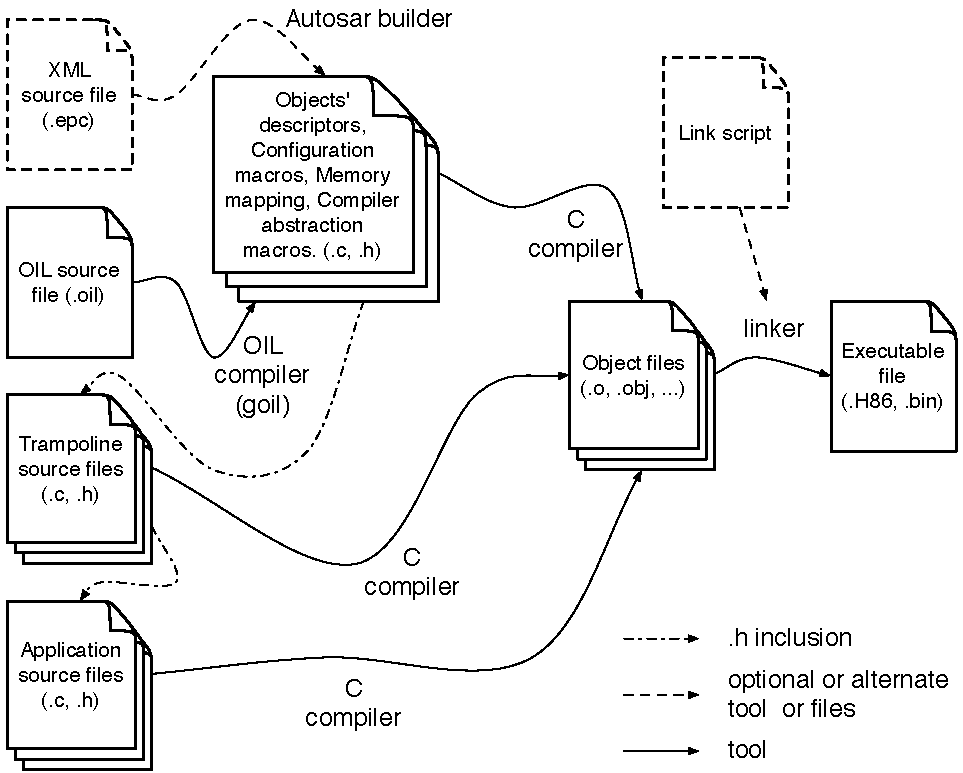
\includegraphics[width=4.3in]{pictures/buildProcess.pdf} 
   \caption{\textbf{Build process of an application with Trampoline.} Starting from the left, the .c and .h corresponding to the application description given in OIL (or XML) are generated by \goil\ (or another system generation tool, for instance an Autosar compliant one) and compiled using a C compiler. Trampoline source files are compiled too and include .h from the description for configuration purpose (see section \ref{sec:configmacros}). Application files are compiled and include .h files from Trampoline. All the object files are then linked together using an optional link script generated by \goil\ or provided with the application.}\label{fig:buildtrampoline}
\end{figure}

\section{The generated files}
\label{sec:generatedfiles}

The following files are generated by \goil\ from the OIL file or should be generated if you use a different system configuration tool. More information may be found in part \ref{part:goil}.

\rowcolors{1}{white}{light-gray}
\begin{longtable}[c]{l|p{4in}}
{\bf File name} & {\bf Usage} \\

\hline

tpl_app_define.h\index{tpl_app_define.h} & This file contains all the configuration macros (see section \ref{sec:configmacros}) and is included in all the Trampoline files to trigger conditional compilation. \goil\ generates this file using the \file{tpl_app_define_h.goilTemplate} template file.\\

tpl_app_config.h\index{tpl_app_config.h} & This file contains the declarations of the constants and functions required by the OSEK and Autosar standard (like OSMAXALLOWEDVALUE_x, OSTICKSPERBASE_x or OSMINCYCLE_x constants for counter x). \goil\ generates this file using the \file{tpl_app_config_h.goilTemplate} template file.\\

tpl_app_config.c\index{tpl_app_config.c} & This file contains the definitions of the constants and functions required by the OSEK and Autosar standard and the definitions of object descriptors used by Trampoline (see section \ref{sec:structs}) \goil\ generates this file using the \file{tpl_app_config_c.goilTemplate} template file.\\

tpl_app_custom_types.h\index{tpl_app_custom_types.h} & Some data types used by Trampoline are not statically defined. They are generated to fit size or performance criterions. For instance, the type used for a TaskType may be a byte if there is less than 256 tasks in the system and a word otherwise. This file defined these data types.\\

tpl_service_ids.h\index{tpl_service_ids.h} & This file is generated only if Trampoline is compiled with service calls implemented using a system call. It contains all the identifiers of the services used by the application according to the configuration. \goil\ generates this file using the \file{tpl_service_ids_h.goilTemplate} template file.\\

tpl_dispatch_table.c\index{tpl_dispatch_table.c} & This file is generated only if Trampoline is compiled with service calls implemented using a system call. It contains the dispatch table definition. See section \ref{sec:dispatchtable}. \goil\ generates this file using the \file{tpl_dispatch_table_c.goilTemplate} template file.\\

tpl_invoque.S\index{tpl_invoque.S} & This file is generated only if Trampoline is compiled with service calls implemented using a system call. It contains the API functions for system services. See section \ref{sec:invoque}. The extension (here .S) may change according to the assembler used. \goil\ generates this file using the \file{tpl_invoque.goilTemplate} and \file{service_call.goilTemplate} template files.\\

MemMap.h\index{MemMap.h} & This file is generated only if memory mapping is enabled. It contains macros for compiler abstraction memory mapping of functions and data as defined in the Autosar standard \cite{autosar31memorymapping}. \goil\ generates this file using the \file{MemMap_h.goilTemplate} template file.\\

Compiler.h\index{Compiler.h} & This file is generated only if memory mapping is enabled. It contains macros for the compiler abstraction of functions and pointer qualifier as defined in the Autosar standard \cite{autosar31compilerabstraction}. \goil\ generates this file using the \file{Compiler_h.goilTemplate} template file.\\

Compiler_Cfg.h\index{Compiler_Cfg.h} & This file is generated only if memory mapping is enabled. It contains macros for the compiler abstraction configuration as defined in the Autosar standard \cite{autosar31compilerabstraction}. \goil\ generates this file using the \file{Compiler_Cfg_h.goilTemplate} template file.\\

script.ld\index{script.ld} & This file is generated only if memory mapping is enabled. It contains a link script to map the executable in the target memory. \goil\ generates this file using the \file{script.goilTemplate} template file.\\

\end{longtable}

The following sections give details about the content of these files.

\section{The Configuration Macros}
\label{sec:configmacros}

Trampoline can be compiled with various options. These options are controlled by setting the appropriate preprocessor configuration macros%
\index{Configuration macros}.
These macros are usually set by \goil
using the template found in \file{tpl_app_define_h.goilTemplate} file to produce the \file{tpl_app_define.h}\index{tpl_app_define.h} file that is included by the files of Trampoline. However, a different generation tool may be used and it should comply to the specification presented in the following tables. When Trampoline is compiled, the coherency and consistency of the configuration macros are checked, by using the preprocessor macros located in the \file{tpl_config_check.h} file, to ensure they correspond to a supported configuration.

3 kinds of configuration macros are used: boolean macros, numerical macros, symbol macros and string macros. Boolean macros may take 2 values: \YES\ or \NO. All macros should be defined, Trampoline does not use the \lstinline[language=C]{#ifdef} or \lstinline[language=C]{\#ifndef} scheme to limit the occurrences of unwanted misconfigurations except to prevent multiple inclusions of the same header file.

\subsection{Number of objects macros}

These macros gives the number of objects of each kind (tasks, ISRs, resources, \ldots) and other values. They are used in Trampoline to check the validity of the various identifiers and to define tables of the corresponding size.
 
\rowcolors{1}{white}{light-gray}
\begin{longtable}[c]{l|l|p{3.5in}}
{\bf Macro}&{\bf Kind}&{\bf Effect}\\
\hline
\idxconfflag{PRIO_LEVEL_COUNT} &  Integer & The number of priority levels used in the system.\\
\idxconfflag{TASK_COUNT} & Integer & The number of tasks (basic and extended) used in the system.\\
\idxconfflag{EXTENDED_TASK_COUNT} & Integer & The number of extended tasks used in the system.\\
\idxconfflag{ISR_COUNT} & Integer & The number of ISR category 2 used in the system.\\
\idxconfflag{ALARM_COUNT} & Integer & The number of alarms used in the system.\\
\idxconfflag{RESOURCE_COUNT} & Integer & The number of resources used in the system.\\
\idxconfflag{SEND_MESSAGE_COUNT} & Integer & The number of send messages used in the system.\\
\idxconfflag{RECEIVE_MESSAGE_COUNT} & Integer & The number of receive messages used in the system.\\
\idxconfflag{SCHEDTABLE_COUNT} & Integer & The number of schedule tables used in the system. This macros is only used when \cmacro{WITH_AUTOSAR} is set to \YES.\\
\idxconfflag{COUNTER_COUNT} & Integer & The number of counters used in the system. This macros is only used when \cmacro{WITH_AUTOSAR} is set to \YES.\\
\idxconfflag{APP_COUNT} & Integer & The number of OS applications used in the system. This macros is only used when \cmacro{WITH_AUTOSAR} is set to \YES.\\
\idxconfflag{TRUSTED_FCT_COUNT} & Integer & The number of trusted functions used in the system. This macros is only used when \cmacro{WITH_AUTOSAR} is set to \YES.\\
\idxconfflag{RES_SCHEDULER_PRIORITY} & Integer & The priority of the \constant{RES_SCHEDULER} resource. This should be equal to the highest priority among the tasks.\\
\end{longtable}

\subsection{Error Handling Macros}
\label{sec:errorhook}

Error handling related macros are used to configure what kind of error Trampoline checks and what extra processing is done when an error is encountered.

\rowcolors{1}{white}{light-gray}
\begin{longtable}[c]{l|l|p{3.3in}}
{\bf Macro} & {\bf Kind} & {\bf Effect}\\
\hline
\idxconfflag{WITH_OS_EXTENDED} & Bool & When set to \YES, Trampoline system services perform error checking on their arguments. \cmacro{WITH_OS_EXTENDED} is set to \YES\ with a \oilattr{STATUS} = \constant{EXTENDED} and is set to \NO\ with a \oilattr{STATUS} = \constant{BASIC} in the OIL OS object.\\
\idxconfflag{WITH_ERROR_HOOK} & Bool & When set to \YES, the \cfunction{ErrorHook()} function is called if an error occurs. \cmacro{WITH_ERROR_HOOK} is set to \YES/\NO\ with a \cmacro{ERRORHOOK} = \TRUE/\FALSE\ in the OIL OS object.\\
\idxconfflag{WITH_USEGETSERVICEID} & Bool & When set to \YES, Trampoline system services store the id of the current service. This id may be retrieved in the \cfunction{ErrorHook()} function by using the \cfunction{OSErrorGetServiceId()} macro. \cmacro{WITH_USEGETSERVICEID} is set to \YES/\NO\ with a \oilattr{USEGETSERVICEID} = \TRUE/\FALSE\ in the OIL OS object.\\
\idxconfflag{WITH_USEPARAMETERACCESS} & Bool & When set to \YES, Trampoline system services store the arguments of the current service. These arguments may be retrieved in the \cfunction{ErrorHook()} function by using the ad-hoc access macros (see \cmacro{WITH_USEGETSERVICEID} above). \cmacro{WITH_USEPARAMETERACCESS} is set to \YES/\NO\ with a \oilattr{USEPARAMETERACCESS} = \TRUE/\FALSE\ in the OIL OS object.\\
\idxconfflag{WITH_COM_ERROR_HOOK} & Bool & When set to \YES, the communication error hook is called when error occurs in the communication sub-system. This macro is only available when \cmacro{WITH_COM} is set to \YES.\\
\idxconfflag{WITH_COM_USEGETSERVICEID} & Bool & When set to \YES, Trampoline/COM system services store the id of the current service. This id may be retrieved in the \cfunction{COMErrorHook()} function by using the \cfunction{COMErrorGetServiceId()} macro. \cmacro{WITH_COM_USEGETSERVICEID} is set to \YES/\NO\ with a \oilattr{COMUSEGETSERVICEID} = \TRUE/\FALSE\ in the OIL COM object.\\
\idxconfflag{WITH_COM_USEPARAMETERACCESS} & Bool & When set to \YES, Trampoline/COM system services store the arguments of the current service. These arguments may be retrieved in the \cfunction{COMErrorHook()} function by using the ad-hoc access macros (see \ref{sec:comerrorhook}). \cmacro{WITH_COM_USEPARAMETERACCESS} is set to \YES/\NO with a \oilattr{COMUSEPARAMETERACCESS} = \TRUE/\FALSE\ in the OIL COM object.\\
\idxconfflag{WITH_COM_EXTENDED} & Bool & When set to \YES, Trampoline/COM system services perform error checking on their arguments. \cmacro{WITH_COM_EXTENDED} is set to \YES\ with a \oilattr{COMSTATUS} = \EXTENDED\ and is set to \NO\ with a \oilattr{COMSTATUS} = \BASIC\ in the OIL COM object.\\
\end{longtable}

\subsection{Protection Macros}
\label{sec:protectionhook}

Protection macros deal with protection facilities provided by the \autosar\ standard.

\rowcolors{1}{white}{light-gray}
\begin{longtable}[c]{l|l|p{3.6in}}
{\bf Macro} & {\bf Kind} & {\bf Effect}\\
\hline
\idxconfflag{WITH_MEMORY_PROTECTION} & Bool & When set to \YES, Trampoline enables the memory protection facility. This is only supported on some ports (MPC5510 and ARM9 at time of writing). Memory protection requires the memory mapping and the use of system call. \cmacro{WITH_MEMORY_PROTECTION} is set to \YES/\NO\ with the \oilattr{MEMORY_PROTECTION} attribute of \oilattr{MEMMAP} object (see \ref{sec:memmap}) set to \TRUE/\FALSE.\\
\idxconfflag{WITH_TIMING_PROTECTION} & Bool & When set to \YES, Trampoline enables the timing protection facility. \cmacro{WITH_TIMING_PROTECTION} is set to \YES if the \oilattr{AUTOSAR_SC} is 2 or 4 (see \ref{sec:autosarsc}) and a least one of the objects specifies a timing protection related attribute in the OIL file.\\
\idxconfflag{WITH_PROTECTION_HOOK} &  Bool & When set to \YES, Trampoline calls the \cfunction{ProtectionHook()} with the appropriate argument when a protection fault occurs. \cmacro{WITH_PROTECTION_HOOK} is set to \YES with a \oilattr{PROTECTIONHOOK} = \TRUE in the OIL OS object.\\
\idxconfflag{WITH_STACK_MONITORING} & Bool & When set to \YES, Trampoline enables the stack monitoring. Each time a context switch occurs, the stack pointer is checked. If the stack pointer is outside the stack zone of the process, a fault occurs. \cmacro{WITH_STACK_MONITORING} is set to \YES with a \oilattr{STACKMONITORING} = TRUE in the oil OS object.\\
\end{longtable}

\subsection{Hook call macros}

Hook call macros control whether a hook is called or not.

\rowcolors{1}{white}{light-gray}
\begin{longtable}[c]{l|l|p{3.71in}}
{\bf Macro} & {\bf Kind} & {\bf Effect}\\
\hline
\idxconfflag{WITH_ERROR_HOOK} & Bool & see \ref{sec:errorhook}\\
\idxconfflag{WITH_PRE_TASK_HOOK} & Bool & When set to \YES, each time a task is scheduled, the function \cfunction{PreTaskHook()} is called. \cmacro{WITH_PRE_TASK_HOOK} is set to \YES/\NO\ with a \oilattr{PRETASKHOOK} = \TRUE/\FALSE\
  in the OIL OS object.\\
\idxconfflag{WITH_POST_TASK_HOOK} & Bool & When set to \YES, each time a task is descheduled, the function \cfunction{PostTaskHook()} is called. \cmacro{WITH_POST_TASK_HOOK} is set to \YES/\NO\ with a \oilattr{POSTTASKHOOK} = \TRUE/\FALSE\
  in the OIL OS object.\\
\idxconfflag{WITH_STARTUP_HOOK} & Bool & When set to \YES, the function \cfunction{StartupHook()} is called within the \api{StartOS} service.  \cmacro{WITH_STARTUP_HOOK} is set to \YES/\NO\ with a \oilattr{STARTUPHOOK} = \TRUE/\FALSE\ in the OIL OS object.\\
\idxconfflag{WITH_SHUTDOWN_HOOK} & Bool & When set to \YES, the function \cfunction{ShutdownHook()} is called within the \api{ShutdownOS} service. \cmacro{WITH_SHUTDOWN_HOOK} is set to \YES/\NO\ with a \oilattr{SHUTDOWNHOOK} = \TRUE/\FALSE\ in the OIL OS object.\\
\idxconfflag{WITH_PROTECTION_HOOK} & Bool & see \ref{sec:protectionhook}\\
\end{longtable}

\subsection{Miscellaneous macros}

Here are the other available macros:

\rowcolors{1}{white}{light-gray}
\begin{longtable}[c]{l|l|p{3.25in}}
{\bf Macro} & {\bf Kind} & {\bf Effect}\\
\hline
\idxconfflag{WITH_USERESSCHEDULER} & Bool & When set to \YES, the \constant{RES_SCHEDULER} resource is used by at least one process. \cmacro{WITH_USERESSCHEDULER} is set to \YES/\NO\ with a \oilattr{USERESSCHEDULER} = \TRUE/\FALSE\ in the OIL OS object.\\
\idxconfflag{WITH_SYSTEM_CALL} & Bool & When set to \YES, services are called by the mean of a system call, also known as a software interrupt (see section \ref{sec:systemcall}). \cmacro{WITH_SYSTEM_CALL} is set to \YES/\NO\ according to the target architecture and requires a memory mapping\\
\idxconfflag{WITH_MEMMAP} & Bool & When set to \YES, a memory mapping is used. A \file{MemMap.h} files giving the available memory segments is included and should be generated or provided by the user. \goil\ generates such a file.
  \cmacro{WITH_MEMMAP} is set to \YES/\NO\ with a \oilattr{MEMMAP} = \TRUE/\FALSE\ in the OIL OS object.\\
\idxconfflag{WITH_COMPILER_SETTINGS} & Bool & When set to \YES, the compiler dependent macros are used. \file{Compiler.h} and \file {Compiler_Cfg.h} files are includes and should be generated or provided by the user. \goil\ generates these  files if \oilattr{MEMMAP} is \TRUE\ and the \oilattr{COMPILER} sub-attribute is set.\\
\idxconfflag{WITH_AUTOSAR} & Bool & When set to \YES, Trampoline contains additional system services, code and declarations related to the \autosar\ standard. For instance, the counter descriptor includes the counter type (hardware or software).   \cmacro{WITH_AUTOSAR} is set to \YES/\NO\ when at least one \autosar\ object is present in the system configuration (OIL file for instance).\\
\idxconfflag{TRAMPOLINE_BASE_PATH} & String & The path to Trampoline root directory.\\
\idxconfflag{AUTOSAR_SC} & Integer & The \autosar\ scalability class\index{Scalability class} ranging from 0 to 4. 0 means OSEK\\
\idxconfflag{WITH_OSAPPLICATION} & Bool & When set to \YES, OS Application\index{OS Application} are used.\\
\idxconfflag{WITH_TRACE} & Bool & When set to \YES, the tracing of the operating system is enabled.\\
\idxconfflag{TRACE_TASK} & Bool & When set to \YES, task (de)scheduling events are traced. Only available if \cmacro{WITH_TRACE} is set to \YES.\\
\idxconfflag{TRACE_ISR} & Bool & When set to \YES, ISR category 2 (de)scheduling events are traced. Only available if \cmacro{WITH_TRACE} is set to \YES.\\
\idxconfflag{TRACE_RES} & Bool & When set to \YES, resources get and release are traced. Only available if \cmacro{WITH_TRACE} is set to \YES.\\
\idxconfflag{TRACE_ALARM} & Bool & When set to \YES, alarm activities are traced. Only available if \cmacro{WITH_TRACE} is set to \YES.\\
\idxconfflag{TRACE_U_EVENT} & Bool & When set to \YES, user events are traced. Only available if \cmacro{WITH_TRACE} is set to \YES.\\
\idxconfflag{TRACE_FORMAT} & Symbol & Trace format. A function named \cfunction{tpl_trace_format_\toreplace{\cmacro{TRACE_FORMAT}}} is expected. Only available if \cmacro{WITH_TRACE} is set to \YES.\\
\idxconfflag{TRACE_FILE} & String & File name where the trace is stored. Usable on Posix target only. Only available if \cmacro{WITH_TRACE} is set to \YES.\\
\idxconfflag{WITH_IT_TABLE} & Bool & When set to \YES, the external interrupts are dispatched using a table of fonction pointers.\\
\idxconfflag{WITH_COM} & Bool & When set to \YES, internal communication is used.\\
\idxconfflag{TPL_COMTIMEBASE} & Integer & The \oilattr{COMTIMEBASE} expressed in nanoseconds.\\
\idxconfflag{WITH_COM_STARTCOMEXTENSION} & Bool & When set to \YES, the communication extension function is called.\\
\end{longtable}

\section{Application configuration}

The application configuration is generated by \goil\ using the template found in \file{tpl_app_config_h.goilTemplate} file and \file{tpl_app_config_c.goilTemplate} file to produce the \file{tpl_app_define.h}\index{tpl_app_define.h} and \file{tpl_app_define.c}\index{tpl_app_define.c} files.

\subsection{Counter related constants declaration}

The \file{tpl_app_config.h} files contains the counters related constants: those of the SystemCounter\footnote{the default counter of an OSEK operating system} and those of the counters defined by the user. The SystemCounter constants are located in the generated files because the SystemCounter default attributes may be modified by the user in the OIL or XML file. The constants of a user defined counter are declared as follow:

\begin{lstlisting}[language=C]
extern CONST(tpl_tick, OS_CONST) OSTICKSPERBASE_<counter name>;
extern CONST(tpl_tick, OS_CONST) OSMAXALLOWEDVALUE_<counter name>;
extern CONST(tpl_tick, OS_CONST) OSMINCYCLE_<counter name>;
\end{lstlisting}

Where \toreplace{counter name} is obviously the name given to the counter in the confguration. For the SystemCounter, the following constants are declared:

%\begin{lstlisting}[language=C]
%extern CONST(tpl_tick, OS_CONST) OSTICKSPERBASE;
%extern CONST(tpl_tick, OS_CONST) OSMAXALLOWEDVALUE;
%extern CONST(tpl_tick, OS_CONST) OSMINCYCLE;
%\end{lstlisting}

\subsection{Events definition}

The \file{tpl_app_config.c} file should contain the event mask definitions. For each event defined in the configuration, the following lines should appear:

\begin{lstlisting}[language=C]
#define API_START_SEC_CONST_UNSPECIFIED
#include "tpl_memmap.h"

#define <event name>_mask <mask value>
CONST(EventMaskType, AUTOMATIC) <event name> = <event name>_mask;

#define API_STOP_SEC_CONST_UNSPECIFIED
#include "tpl_memmap.h"
\end{lstlisting}

Where \toreplace{event name} is the name given to the event in the configuration and \toreplace{mask value} is the value set by the user in the configuration or, when set to AUTO, the value computed by the generation tool.

\subsection{Standard resources definition}

Standard resources need the definition of an identifier used to reference the resource in a system service (\cfunction{GetResource()} and \cfunction{ReleaseResource()}) and an instance of a \ctype{tpl_resource} structure (see \ref{sec:structtplresource}). This is done with the following definitions:

\begin{lstlisting}[language=C]
#define API_START_SEC_CONST_UNSPECIFIED
#include "tpl_memmap.h"

#define <resource name>_id <resource id>
CONST(ResourceType, AUTOMATIC) <resource name> = <resource name>_id;

#define API_STOP_SEC_CONST_UNSPECIFIED
#include "tpl_memmap.h"

#define OS_START_SEC_VAR_UNSPECIFIED
#include "tpl_memmap.h"

VAR(tpl_resource, OS_VAR) <resource name>_rez_desc = {
  /* ceiling priority of the resource */  <resource priority>,
  /* owner previous priority          */  0,
  /* owner of the resource            */  INVALID_PROC_ID,
#if WITH_OSAPPLICATION == YES
  /* OS Application id                */  <resource application id>,
#endif    
  /* next resource in the list        */  NULL
};

#define OS_STOP_SEC_VAR_UNSPECIFIED
#include "tpl_memmap.h"
\end{lstlisting}

Where \toreplace{resource name} is the name given to the resource in the configuration, \toreplace{resource priority} is the priority of the resource that is computed by the generation tool and is the maximum priority of the processes that use the resource and \toreplace{resource application id} is the identifier of the OS Application the resource belongs to. Since this field is protected by \var{WITH_OSAPPLICATION}, it may be leaved empty when no OS Application is used.

\toreplace{resource id} ranges from 0 to the number of standard resources minus 1. Once every standard resource descriptor is defined, a table gathering pointers to the resource descriptors and indexed by the resource id has to be defined. This table is used by system services to get the resource descriptor from the resource id. Suppose 3 standard resource, \var{motor1}, \var{motor2} and \var{dac} has been defined and RES_SCHEDULER is used, the table should be as follow:

\begin{lstlisting}[language=C]
#define OS_START_SEC_CONST_UNSPECIFIED
#include "tpl_memmap.h"
CONSTP2VAR(tpl_resource, AUTOMATIC, OS_APPL_DATA)
tpl_resource_table[RESOURCE_COUNT] = {
  &motor1_rez_desc,
  &motor2_rez_desc,
  &dac_rez_desc,
  &res_sched_rez_desc  
};
#define OS_STOP_SEC_CONST_UNSPECIFIED
#include "tpl_memmap.h"
\end{lstlisting}

\var{\&res_sched_rez_desc}, the pointer to the resource descriptor of RES_SCHEDULER should always be the last element of the table. If RES_SCHEDULER is not used, simply remove it from the table.

\subsection{Tasks definition}

Each task needs an identifier to reference a task un a system service (\cfunction{ActivateTask()}, \cfunction{ChainTask()}, \cfunction{GetTaskState()}, \cfunction{SetEvent()} and \cfunction{GetEvent()}) and the declaration of the task function. The following definitions should appear for each task:

\begin{lstlisting}[language=C]
#define API_START_SEC_CONST_UNSPECIFIED
#include "tpl_memmap.h"

#define <task name>_id <task id>
CONST(TaskType, AUTOMATIC) <task name> = <task name>_id;

#define API_STOP_SEC_CONST_UNSPECIFIED
#include "tpl_memmap.h"

#define APP_Task_<task name>_START_SEC_CODE
#include "tpl_memmap.h"

FUNC(void, OS_APPL_CODE) <task name>_function(void);

#define APP_Task_<task name>_STOP_SEC_CODE
#include "tpl_memmap.h"
\end{lstlisting}

Where \toreplace{task name} is the name given to the task in the configuration and \toreplace{task id} is the identifier of the task computed by the system generation tool. Task ids should range from 0 to the number of tasks minus 1. In addition, id allocation must start with extended tasks first and basic task after. In addition an instance of the static task descriptor must be provided:

\begin{lstlisting}[language=C]
#define OS_START_SEC_CONST_UNSPECIFIED
#include "tpl_memmap.h"
CONST(tpl_proc_static, OS_CONST) <task name>_task_stat_desc = {
  /* context                  */  <task name>_CONTEXT,
  /* stack                    */  <task name>_STACK,
  /* entry point (function)   */  <task name>_function,
  /* internal ressource       */  <internal resource>,
  /* task id                  */  <task name>_id,
#if WITH_OSAPPLICATION == YES
  /* OS application id        */  <application>,
#endif
  /* task base priority       */  <task priority>,
  /* max activation count     */  <task activation>,
  /* task type                */  <task type>
#if WITH_AUTOSAR_TIMING_PROTECTION == YES
  /* pointer to the timing
     protection descriptor    */  ,<timing protection>
#endif
};
#define OS_STOP_SEC_CONST_UNSPECIFIED
#include "tpl_memmap.h"
\end{lstlisting}

Where \toreplace{task name} is the name given to the task in the configuration. \toreplace{internal resource} mays be one of the following:

\begin{itemize}
\item a pointer to the internal resource descriptor (see \ref{sec:internalresource}) if an internal resource has been defined in the configuration;
\item a pointer to the scheduler internal resource if the task has been defined as non-preemptable in the configuration;
\item NULL if none of the above cases apply.
\end{itemize}

\toreplace{application} is the id of the OS Application the task belongs to when OS Application are used or, when they are not used, nothing at all. \toreplace{task priority} is the priority of the task as computed by the \sysgen. \toreplace{task activation} is the maximum number of task activation allowed as defined in the configuration. \toreplace{task type} may be \EXTENDED\ or \BASIC. \toreplace{timing protection} is a pointer to the timing protection descriptor or NULL if no timing protection is defined for the task.

Also an instance of the dynamic task descriptor must be provided:

\begin{lstlisting}[language=C]
#define OS_START_SEC_VAR_UNSPECIFIED
#include "tpl_memmap.h"

VAR(tpl_proc, OS_VAR) <task name>_task_desc = {
  /* resources                      */  NULL,
#if WITH_MEMORY_PROTECTION == YES
  /* if > 0 the process is trusted  */  <trusted count>,    
#endif /* WITH_MEMORY_PROTECTION */
  /* activate count                 */  0,
  /* task priority                  */  <task priority>,
  /* task state                     */  <task state>
#if WITH_AUTOSAR_TIMING_PROTECTION == YES
  /* activation allowed             */  ,TRUE
#endif
};

#define OS_STOP_SEC_VAR_UNSPECIFIED
#include "tpl_memmap.h"
\end{lstlisting}

Where \toreplace{task name} is the name given to the task in the configuration. \toreplace{trusted count} is 0 if the task belongs to a non trusted OS Application and 1 if the tasks belongs to a trusted OS Application. \toreplace{task priority} is the priority of the task as computed by the \sysgen. \toreplace{task state} is the initial state of the task and must be set to AUTOSTART or SUSPENDED.

If the task is an EXTENDED one, an event mask descriptor is added:

%\lstdefinelanguage[trampconf]{C}{morecomment=[s][\color{red}]{<}{>}}

\begin{lstlisting}[language=C]
VAR(tpl_task_events, OS_VAR) <task name>_task_evts = {
  /* event set  */ 0,
  /* event wait */ 0
};
\end{lstlisting}

Where \toreplace{task name} is the name given to the task in the configuration.


%!TEX root = ./main.tex

\chapter{Kernel Implementation}

\section{The \var{tpl_kern} structure}

The \var{tpl_kern} structure gathers informations about the \RUNNING\ process and flags to notify if a context switch and/or a context save are needed. It eases the access to these informations when programming in assembly language. The \var{tpl_kern} structure is an instance of the \ctype{tpl_kern_state} type:

\begin{lstlisting}[language=C]
typedef struct 
{
  P2CONST(tpl_proc_static, TYPEDEF, OS_CONST) s_old;
  P2CONST(tpl_proc_static, TYPEDEF, OS_CONST) s_running;
  P2VAR(tpl_proc, TYPEDEF, OS_VAR)            old;
  P2VAR(tpl_proc, TYPEDEF, OS_VAR)            running;
  VAR(int, TYPEDEF)                           running_id;
  VAR(u8, TYPEDEF)                            need_switch;
} tpl_kern_state;
\end{lstlisting}

\section{Ready list implementation}

The implementation of the ready list makes it possible to reconcile relative simplicity with good performance regardless of the number of processes\footnote{The term process here refers to a task or an SRI2}. The ready list is implemented by an array indexed by priority. Each element of this array is a FIFO that stores the process identifier. An activated process is stored at the tail of the FIFO. A pre-empted process is stored at the head of the FIFO. Furthermore, in order to quickly find the non-empty FIFO corresponding to the highest priority, a binary heap is used to store the indexes (i.e. priority) of the non-empty FIFOs, the highest index being of course at the root of the heap.
 
FIFO sizes are determined during the OIL compilation. Once the priorities assigned to processes and resources are determined, the FIFO size corresponding to a priority is the sum of the activations of each task, the number of resources and the number of ISR2 for this priority. Priority level 0 is only occupied by the task \emph{idle}.

Let's take for example an application composed of 4 tasks and 2 resources, declared in OIL file as shown below.

\begin{lstlisting}[language=OIL]
RESOURCE r1 { RESOURCEPROPERTY = STANDARD; };
RESOURCE r2 { RESOURCEPROPERTY = STANDARD; };
TASK t1 { PRIORITY = 2; ACTIVATION = 2; RESOURCE = r1; };
TASK t2 { PRIORITY = 3; ACTIVATION = 1; };
TASK t3 { PRIORITY = 1; ACTIVATION = 3; RESOURCE = r2; };
TASK t4 { PRIORITY = 1; ACTIVATION = 2; RESOURCE = r1; RESOURCE = r2; };
\end{lstlisting} 

The missing attributes for all tasks are \oilattr{SCHEDULE = FULL} and \oilattr{AUTOSTART = FALSE}. 

The OIL compiler calculates the priority of the resource \oilval{r1}. As it is likely to be taken by the tasks \oilval{t1} and \oilval{t4}, its calculated priority is 3 (1 higher than the maximum priorities of \oilval{t1} and \oilval{t4}). Therefore the priority of \oilval{t2} is increased by 1 to allow it to pre-empt \oilval{t1} or \oilval{t4} when it holds the resource. The same is done for \oilval{r2}, which leads to give it the priority of 2. Consequently, the priorities of \oilval{t1}, \oilval{t2} and \oilval{r1} are increased by 1 to make room for \oilval{r2}. The occupancy of the priority levels and the corresponding size of the FIFO is therefore as shown in the table \ref{tab:example-fifo}:

% Requires the booktabs if the memoir class is not being used
\begin{table}[htbp]
   \centering
   %\topcaption{Table captions are better up top} % requires the topcapt package
   \begin{tabular}{|llc|} % Column formatting, @{} suppresses leading/trailing space
      \hline
      Priority level    & Content & FIFO size\\
      \hline
      0 & \emph{idle} & 1\\
      1 & \oilval{t3}, \oilval{t4} & 5\\
      2 & \oilval{r2} & 1\\
      3 & \oilval{t1} & 2\\
      4 & \oilval{r1} & 1\\
      5 & \oilval{t2} & 1\\
      \hline
   \end{tabular}
   \caption{Priority levels and FIFO size for the example.}
   \label{tab:example-fifo}
\end{table}% Requires the booktabs if the memoir class is not being used

The data structure for this example is given in figure \ref{fig:array-fifo}. 

\begin{figure}[htbp] %  figure placement: here, top, bottom, or page
   \centering
   \begin{tikzpicture}[yscale=-.8,xscale=.8]
   \draw (-.5,2.5) node[anchor=south, rotate=90] {Priority};
   \foreach \index/\size in {0/1,1/5,2/1,3/2,4/1,5/1} {
      \draw (0,\index) node {\index};
      \draw ($(0,\index)+(.5,-.5)$) rectangle ++(1,1);
      \filldraw ($(0,\index)+(1,0)$) circle (.1);
      \draw[->] ($(0,\index)+(1,0)$) -- ++(1,0);
      \foreach \f in {1,...,\size} {
        \draw ($(.7*\f+.3,\index)+(1,-.4)$) rectangle ++(.7,.7);
      }
   }
   \end{tikzpicture}
   \caption{Data structure for the example.}
   \label{fig:array-fifo}
\end{figure}
\documentclass[11pt, oneside]{article}   	% use "amsart" instead of "article" for AMSLaTeX format
\usepackage{geometry}                		% See geometry.pdf to learn the layout options. There are lots.
\geometry{letterpaper}                   		% ... or a4paper or a5paper or ... 
%\geometry{landscape}                		% Activate for for rotated page geometry
%\usepackage[parfill]{parskip}    		% Activate to begin paragraphs with an empty line rather than an indent
\usepackage{graphicx}				% Use pdf, png, jpg, or eps§ with pdflatex; use eps in DVI mode
								% TeX will automatically convert eps --> pdf in pdflatex		
\usepackage{amssymb}
\usepackage[utf8]{inputenc}
\usepackage{listings}
\usepackage{hyperref}
\usepackage{tikz}
\usetikzlibrary{patterns,calc}

\newcommand{\sch}{\lstinline{tpl_sc_handler}}

\title{MSP430X port - small memory model version}
\author{Jean-Luc Béchennec}
%\date{}							% Activate to display a given date or no date

\lstset{% general command to set parameter(s)
	basicstyle=\footnotesize\ttfamily,
	backgroundcolor=\color{lightgray!30},
	frame=single, framerule=0pt
}

\begin{document}
\maketitle

This document describes the small version for the CPUX of the Trampoline port on MSP430, which assumes that the code is hosted in the first 64kB of memory and therefore the addresses are stored on 16-bit words. Instruction set of the MSP430X is available in \cite{slau208q} or \cite{slau367o}.

\section{ABI}

In \cite{slaa664} a change has been made in GCC so that it conforms to the ABI defined in \cite{slaa534} and becomes compatible with the proprietary Texas Instruments compiler. So there are two GCC compilers for MSP430: the one that does not conform to the ABI defined by Texas Instruments, \emph{MSPGCC}, and the one that does conform to the ABI, \emph{GCC compiler for MSP}. 

As it is difficult to support both ABIs simultaneously, it was decided to support both ABIs at compile time. A precompiled \emph{MSPGCC} is available in the latest version of Energia\footnote{GCC 4.6.3.}. Energia can be downloaded at {\small\url{https://energia.nu}}. A precompiled \emph{GCC compiler for MSP} is available at {\small\url{http://www.ti.com/tool/msp430-gcc-opensource}}.

In both ABIs the registers used to pass arguments to functions are \lstinline{r12}, \lstinline{r13}, \lstinline{r14} and \lstinline{r15}. In the ABI of \emph{MSPGCC}, \lstinline{r15} is the first argument, \lstinline{r14} the second and so on. If a function returns a value, it is placed in \lstinline{r15}. In the ABI of \emph{GCC compiler for MSP} \lstinline{r12} is the first argument, \lstinline{r13} the second and so on. If a function returns a value, it is placed in \lstinline{r12}.
 No Trampoline service uses more than 3 arguments and therefore \lstinline{r12}, for \emph{MSPGCC} ABI, or \lstinline{r15}, for \emph{GCC compiler for MSP} ABI, is available to pass the service ID into the wrapper.
 
Adapting to both ABIs at compile time is not very complicated. This involves exchanging the use made of the registers \lstinline{r12}, identifying the service, and \lstinline{r15}, the return value of the service and the argument of \lstinline{tpl_run_elected}. This can be done by defining an abstract register to pass the service identifier and an abstract register to return the return value of the service. The register selection can be made using the preprocessor and the macro \lstinline{__GXX_ABI_VERSION} as shown at Figure \ref{lst:macroabi}. This macro is \lstinline{1002} for \emph{MSPGCC} and \lstinline{1011} for \emph{GCC compiler for MSP}. 2 abstract registers are defined: \lstinline{REG_SID} which is \lstinline{r12} in \emph{MSPGCC} ABI and \lstinline{r15} in \emph{GCC compiler for MSP} ABI, and \lstinline{REG_RETARG} which is \lstinline{r15} in \emph{MSPGCC} ABI and \lstinline{r12}  in \emph{GCC compiler for MSP} ABI.

\begin{figure}[h]
\caption{ABI selection with C preprocessor macros}
\begin{lstlisting}
#if __GXX_ABI_VERSION == 1002
/* MSPGCC ABI */
#define MSPGCC_ABI
#define REG_SID r12
#define REG_RETARG r15
#elif __GXX_ABI_VERSION == 1011
/* GCC compiler for MSP ABI */
#define GCCFORMSP_ABI
#define REG_SID r15
#define REG_RETARG r12
#else
#error "Unsupported ABI"
#endif
\end{lstlisting}
\label{lst:macroabi}
\end{figure}

The following table summarizes the use of the registers in both ABIs if we consider all arguments are small enough to be stored in one register. Although \lstinline{r11} is volatile in one of them, for simplification purposes later on, \lstinline{r11} is considered as non-volatile. A preserved register is noted P and a Volatile register is noted V.

\begin{center}
\begin{tabular}{|l|c|c|}
\hline
Register & \emph{MSPGCC} & \emph{GCC compiler for MSP} \\
\hline
\hline
\lstinline|r0| & \multicolumn{2}{c|}{Program Counter, saved on stack by cpu} \\
\hline
\lstinline|r1| & \multicolumn{2}{c|}{Stack Pointer} \\
\hline
\lstinline|r2| & \multicolumn{2}{c|}{Status Register} \\
\hline
\lstinline|r3| & \multicolumn{2}{c|}{Constants Generator} \\
\hline
\lstinline|r4-r10| & \multicolumn{2}{c|}{Not preserved by the callee} \\
\hline
\lstinline|r11| & V & P \\
\hline
\lstinline|r12| & V, argument 4 & V, argument 1, return value \\
\hline
\lstinline|r13| & V, argument 3 & V, argument 2 \\
\hline
\lstinline|r14| & V, argument 2 & V, argument 3 \\
\hline
\lstinline|r15| & V, argument 1, return value & V, argument 4 \\
\hline
\end{tabular}
\end{center}


It can be noted that the arguments being passed through the low weight 16 bits of the registers, except perhaps for the far pointers, the arguments of the Trampoline services must fit on 16 bits. This limits the tick argument of the services related to alarms to 16 bits. 

% Some Trampoline services use a pointer as an argument: \lstinline{GetTaskId}, \lstinline{GetTaskState}, \lstinline{GetAlarmBase}, \lstinline{GetAlarm}, \lstinline{GetEvent}, \lstinline{SendMessage}, \lstinline{ReceiveMessage}, \lstinline{GetCounterValue}, \lstinline{GetScheduleTableStatus} and \lstinline{GetApplica-}    \lstinline{tionState}. Since none of these services uses more than 2 arguments, a pointer to a high address will occupy 2 registers and the other argument only one. An AUTOSAR service is a problem: \lstinline{GetElapsedCounterValue}. This service takes 3 arguments, two of which are pointers. If the pointed data are in high addresses, some of the arguments will be passed through the stack. However, by forcing the storage of application data whose pointers have been passed to the OS in the lower memory, only 3 registers will be used. Not doing so would lead to unreasonable complexity of wrappers and of the services handler.

\section{Stack}
%\subsection{}

A service call is done using the \lstinline{CALLA} instruction in the service call wrapper. The service identifier is passed to the service call handler through the \lstinline{REG_SID} register. So a service call wrapper is as shown in listing at figure \ref{lst:wrapper}.

\begin{figure}[h]
\caption{Service wrapper}
\begin{lstlisting}
    mov  #<service_id>, REG_SID /* put the service id in the ad-hoc reg */
    call #tpl_sc_handler        /* call the service call handler        */
    ret                         /* return to the caller                 */
\end{lstlisting}
\label{lst:wrapper}
\end{figure}

When in the \sch\ the stack is as shown at figure \ref{fig:stacksc}\footnote{stacks are drawn with the lower address up so they are growing upward, not downward. Each stack location is a 16 bits word.}. \texttt{PTOS} stands for \emph{Process Top Of Stack}.

\begin{figure}[h]
\caption{Stack at beginning of \sch}
\centering
\vspace{1em}
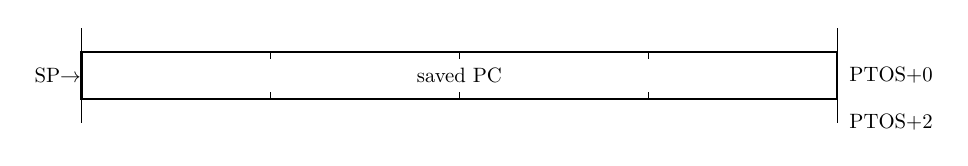
\begin{tikzpicture}[scale=0.6, every node/.style={scale=0.75}]
\draw[thick] (0,3) rectangle ++(16,1); \node at (8,3.5) {saved PC};
\foreach \x in {4,8,12} { \draw (\x,3) -- ++(0,.15);  \draw (\x,4) -- ++(0,-.15); }
%\draw[thick] (0,2) rectangle ++(16,1); \node at (14,2.5) {saved PC [19..16]};
%\draw[thick] (0,1) rectangle ++(16,1); \node at (8,1.5) {service identifier};
%\foreach \x in {4,8,12} { \draw (\x,1) -- ++(0,.15);  \draw (\x,2) -- ++(0,-.15); }
%\draw[thick] (0,0) rectangle ++(16,1); \node at (14,.5) {saved r11 [19..16]};
%\draw (12,0) -- ++(0,1);
%\draw[pattern=north west lines, pattern color=purple] (0,0) rectangle ++(12,1);
%\draw[pattern=north west lines, pattern color=purple] (0,2) rectangle ++(12,1);
\foreach \x in {0,16} \draw (\x,2.5) -- (\x,4.5);
\node at (-.5,3.5) {SP$\rightarrow$};
\foreach \y/\offset in {3.5/0,2.5/2} \node[anchor=west] at (16.1,\y) {PTOS+\offset};
\end{tikzpicture}
\label{fig:stacksc}
\end{figure}

When an interrupt is taken into account, the \lstinline{PC} and the \lstinline{SR} are pushed on the stack. To save space, the \lstinline{SR} is stored in the same 16-bit word as bits 19..16 of \lstinline{PC}. For an obscure reason, words are in reverse order and bits 19..16 of \lstinline{PC} are in high bits. Since all the code is in the first 64kb of the memory, bits 19 to 16 of the PC are always 0. The stack is shown at figure \ref{fig:stackit}.

\begin{figure}[h]
\caption{Stack in an interrupt handler}
\centering
\vspace{1em}
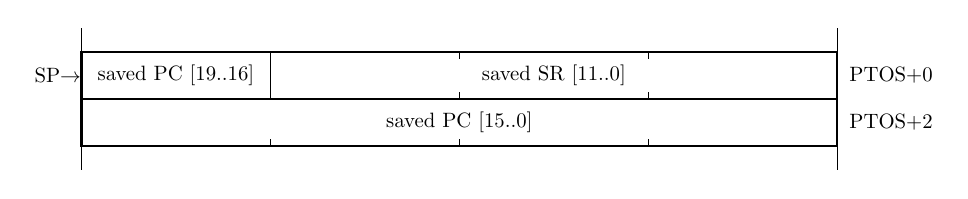
\begin{tikzpicture}[scale=0.6, every node/.style={scale=0.75}]
\draw[thick] (0,2) rectangle ++(16,1); \node at (8,2.5) {saved PC [15..0]};
\foreach \x in {4,8,12} { \draw (\x,2) -- ++(0,.15);  \draw (\x,4) -- ++(0,-.15); }
\draw[thick] (0,3) rectangle ++(16,1); \node at (2,3.5) {saved PC [19..16]}; \node at (10,3.5) {saved SR [11..0]};
\foreach \x in {4,8,12} { \draw (\x,3) -- ++(0,.15);  \draw (\x,4) -- ++(0,-.15); }
%\draw[thick] (0,1) rectangle ++(16,1); \node at (8,1.5) {saved r11 [15..0]};
%\foreach \x in {4,8,12} { \draw (\x,1) -- ++(0,.15);  \draw (\x,2) -- ++(0,-.15); }
%\draw[thick] (0,0) rectangle ++(16,1); \node at (14,.5) {saved r11 [19..16]};
\draw (4,3) -- ++(0,1);
%\draw[pattern=north west lines, pattern color=purple] (0,0) rectangle ++(12,1);
%\draw[pattern=north west lines, pattern color=purple] (0,2) rectangle ++(12,1);
\foreach \x in {0,16} \draw (\x,1.5) -- (\x,4.5);
\node at (-.5,3.5) {SP$\rightarrow$};
\foreach \y/\offset in {3.5/0,2.5/2} \node[anchor=west] at (16.1,\y) {PTOS+\offset};
\end{tikzpicture}
\label{fig:stackit}
\end{figure}

\subsection*{Preemption cases}

A preemption can be synchronous or asynchronous. A synchronous preemption (SP) happens when a service call is done, for instance when a task activates a higher priority task. An asynchronous preemption (AP) happens under interrupt, for instance when a higher priority task is activated by an alarm. A preempted task may resume its execution following a synchronous event (SR) : the running task calls \lstinline{TerminateTask}, \lstinline{ChainTask}, \lstinline{WaitEvent} or \lstinline{SetEvent} or following an asynchronous event (AR) : an alarm does a \lstinline{SetEvent}. So there are 4 cases:.

\begin{description}

\item[SPSR] Synchronous Preemption, Synchronous Resume. $\tau_1$ is running, $\tau_2$ is ready. $P(\tau_1) > P(\tau_2)$.
$\tau_1$ calls \lstinline{WaitEvent} and is preempted synchronously, $\tau_2$ becomes running and  calls \lstinline{SetEvent}. $\tau_2$ is preempted and $\tau_1$ is resumed synchronously.

\item[SPAR] Synchronous Preemption, Asynchronous Resume. $\tau_1$ calls \lstinline{WaitEvent} ans is synchronously preempted, An alarm does a \lstinline{SetEvent} on $\tau_1$ which is asynchronously resumed.

\item[APSR] Asynchronous Preemption, Synchronous Resume. $\tau_1$ is running, $\tau_2$ is suspended. $P(\tau_1) < P(\tau_2)$. An alarm activates $\tau_2$, $\tau_1$ is asynchronously preempted, $\tau_2$ calls \lstinline{TerminateTask}, $\tau_1$ is synchronously resumed.

\item[APAR] Asynchronous Preemption, Asynchronous Resume. $\tau_1$ is running, $\tau_2$ is suspended. $P(\tau_1) < P(\tau_2)$. An alarm activates $\tau_2$, $\tau_1$ is asynchronously preempted. $\tau_2$ is terminated by the OS because of protection fault, for instance a timing protection interrupt and $\tau_1$ is asynchronously resumed.

\end{description}

So \emph{the stack frame has to be normalized}. The normalized stack frame is the asynchronous one shown at figure \ref{fig:stackit} because it contains the Status Register. Normalization is done at the beginning of the \sch. The end of the \sch is done using the \texttt{reti} instruction, as at the end of an interrupt.

The normalized stack frame may be done only when a context is saved to prevent a normalization if there is no context switch. However, the load of the context is much complicated, as the restauration of \texttt{r2} (aka status register) in the \sch re-enable the interrupts before the end of the function.

\section{The tpl\_sc\_handler}

The background color of the code snippets depends on the current active stack:
\begin{description}
	\item[green] process stack
	\item[red]   kernel stack
	\item[yellow] either kernel or process stack
\end{description}

%\fbox{\parbox{.99\textwidth}{The stack structure should be reviewed for the \lstinline{tpl_sc_handler}. Since volatile registers must be stacked first by an ISR, they should be at the bottom of the stack, just above the PC, and not at the top.}}

\vspace{1em}

The first thing to do is to compare the service id to the number of services to verify its validity.

\begin{lstlisting}[backgroundcolor=\color{yellow!15}]
    cmp   #SYSCALL_COUNT, REG_SID
    jlo   tpl_sc_handler_id_ok                /* continue if lower        */
    ret                                       /* return if higher or same */
tpl_sc_handler_id_ok:
\end{lstlisting}

Check the reentrancy counter. If it is not zero, it means the service is called from a hook and has to be processed differently.

\begin{lstlisting}[backgroundcolor=\color{yellow!15}]
    tst.b &tpl_reentrancy_counter
    jnz   tpl_sc_handler_from_hook
    inc.b &tpl_reentrancy_counter     /* It is zero, so it is incremented */
\end{lstlisting}


We need to have the same stack pattern for both the \sch\ and an interrupt handler which calls the operating system. So we push the SR and we reset the 4 higher bits (high weight of PC). Interrupts are disabled so that the kernel cannot be interrupted.

\begin{lstlisting}[backgroundcolor=\color{yellow!15}]
    push  sr
    bic.b #0xF0,1(sp)              /* reset the 4 higher bits of saved SR */
    dint
\end{lstlisting}

The stack is then as follow:

\begin{center}
\begin{tikzpicture}[xscale=0.6,yscale=-0.6, every node/.style={scale=0.75}]
\draw[thick] (0,1) rectangle ++(16,1); \node at (8,1.5) {saved PC};
\draw[thick] (0,0) rectangle ++(16,1); \node at (10,0.5) {saved SR}; \node at (2,0.5) {0 0 0 0};
\draw (4,0) -- ++(0,1);
\foreach \y in {0,1} {
	\foreach \x in {4,8,12} { \draw (\x,\y) -- ++(0,.15);  \draw ($(\x,\y+1)$) -- ++(0,-.15); }
}
%\draw[thick] (0,2) rectangle ++(16,1); \node at (14,2.5) {saved PC [19..16]};
%\draw[thick] (0,1) rectangle ++(16,1); \node at (8,1.5) {service identifier};
%\foreach \x in {4,8,12} { \draw (\x,1) -- ++(0,.15);  \draw (\x,2) -- ++(0,-.15); }
%\draw[thick] (0,0) rectangle ++(16,1); \node at (14,.5) {saved r11 [19..16]};
%\draw (12,0) -- ++(0,1);
%\draw[pattern=north west lines, pattern color=purple] (0,0) rectangle ++(12,1);
%\draw[pattern=north west lines, pattern color=purple] (0,2) rectangle ++(12,1);
\foreach \x in {0,16} \draw (\x,-0.5) -- (\x,2.5);
\node at (-.5,0.5) {SP$\rightarrow$};
\foreach \offset in {0,2} \node[anchor=west] at ($(16.1,.5+.5*\offset)$) {PTOS+\offset};
\end{tikzpicture}
\end{center}

Obviously volatile registers (r12 to r15 because we take into account both ABIs) are not saved in \sch\ since the caller does not expect their values to be preserved but we need to make room (8 bytes) on the stack for them because an interrupt handler will save these registers at this location. The 16 bit words at the bottom of this area is for the \lstinline{REG_RETARG} which is not saved yet.

\begin{lstlisting}[backgroundcolor=\color{yellow!15}]
    sub  #8, r1
\end{lstlisting}

The \sch\ needs one working register and we choose to use \lstinline{r11} which has to be saved on the process stack before using it.

\begin{lstlisting}[backgroundcolor=\color{yellow!15}]
    push r11
\end{lstlisting}

At that stage the stack is shown in figure \ref{fig:stackShapeBeforeCallingService}.

\begin{figure}[t]
\caption{Stack shape before calling the service}
\begin{center}
\begin{tikzpicture}[xscale=0.6, yscale=-.6, every node/.style={scale=0.75}]
\draw[thick] (0,0) rectangle ++(16,1); \node at (8,0.5) {saved r11};
\draw[thick] (0,6) rectangle ++(16,1); \node at (8,6.5) {saved PC};
\draw[thick] (0,5) rectangle ++(16,1); \node at (10,5.5) {saved SR}; \node at (2,5.5) {0 0 0 0};
\draw (4,5) -- ++(0,1);
\foreach \y in {5,6} {
	\foreach \x in {4,8,12} { \draw (\x,\y) -- ++(0,.15);  \draw ($(\x,\y+1)$) -- ++(0,-.15); }
}
%\draw[thick] (0,5) rectangle ++(16,1); \node at (8,5.5) {saved PC [15..0]};
%\foreach \x in {4,8,12} { \draw (\x,6) -- ++(0,.15);  \draw (\x,7) -- ++(0,-.15); }
%\draw[thick] (0,6) rectangle ++(16,1); \node at (14,6.5) {saved PC [19..16]};% \node at (10,5.5) {saved SR [11..0]};
%\draw[pattern=north west lines, pattern color=purple] (0,6) rectangle ++(12,1);
%\foreach \x in {4,8,12} { \draw (\x,5) -- ++(0,.15);  \draw (\x,6) -- ++(0,-.15); }
%\draw (12,6) -- ++(0,1);
\foreach \y in {1,2,3} {
\draw[thick] (0,\y) rectangle ++(16,1); \node at ($(8,\y+.5)$) {space of arg};
}
\draw[thick] (0,4) rectangle ++(16,1); \node at ($(8,4.5)$) {space of arg - will hold {\small REG\_RETARG}};
\foreach \x in {0,16} \draw (\x,-.5) -- (\x,7.5);
\node at (-.5,0.5) {SP$\rightarrow$};
\foreach \offset in {0,2,...,12} \node[anchor=west] at ($(16.1,.5+.5*\offset)$) {PTOS+\offset};
\end{tikzpicture}
\end{center}
\label{fig:stackShapeBeforeCallingService}
\end{figure}



%The bottom of the stack have to be updated to the normalized stack (i.e. the stack in an interrupt handler, figure \ref{fig:stackit}).
%
%\begin{lstlisting}[backgroundcolor=\color{yellow!15}]
%    mov     12(r1), r11    /* Saved PC [19..16] -> r11                  */
%    mov     10(r1), 12(r1) /* Copy saved PC [15..0] at the good place   */
%    swpb    r11            /* Get saved PC [19..16] in bits 11..8       */
%    rlam.w  #4, r11        /* Shift them to bits 19..16                 */
%    bis     r2, r11        /* Add the SR in its location at 11..0       */
%    bis     #8, r11        /* set GIE bit (reset just before with dint) */
%    mov     r11, 12(r1)    /* The stack is ok                           */
%\end{lstlisting}
%
%The stack is then as shown at figure \ref{fig:contextBottom}.
%
%\begin{figure}[h!]
%\caption{Bottom of the context saved on stack}
%\begin{center}
%\begin{tikzpicture}[xscale=0.6, yscale=-.6, every node/.style={scale=0.75}]
%\draw[thick] (0,0) rectangle ++(16,1); \node at (8,0.5) {saved r11};
%\draw[thick] (0,6) rectangle ++(16,1); \node at (8,6.5) {saved PC [15..0]};
%\foreach \x in {4,8,12} { \draw (\x,6) -- ++(0,.15);  \draw (\x,7) -- ++(0,-.15); }
%\draw[thick] (0,5) rectangle ++(16,1); \node at (2,5.5) {saved PC [19..16]}; \node at (10,5.5) {saved SR [11..0]};
%\foreach \x in {8,12} { \draw (\x,5) -- ++(0,.15);  \draw (\x,6) -- ++(0,-.15); }
%\draw (4,5) -- ++(0,1);
%\foreach \y in {1,2,3} {
%\draw[thick] (0,\y) rectangle ++(16,1); \node at ($(8,\y+.5)$) {space of arg};
%}
%\draw[thick] (0,4) rectangle ++(16,1); \node at ($(8,4.5)$) {space of arg - will hold {\small REG\_RETARG}};
%\foreach \x in {0,16} \draw (\x,-.5) -- (\x,7.5);
%\node at (-.5,0.5) {SP$\rightarrow$};
%\foreach \offset in {0,2,...,12} \node[anchor=west] at ($(16.1,.5+.5*\offset)$) {PTOS+\offset};
%\end{tikzpicture}
%\end{center}
%\label{fig:contextBottom}
%\end{figure}

Before calling the service, we setup the kernel stack. The process stack pointer (PSP) is saved in r11, then SP is loaded to the kernel stack bottom and the PSP is saved on the kernel stack.

\begin{lstlisting}[backgroundcolor=\color{red!15}]
    mov  r1,r11
    mov  #tpl_kern_stack_bottom, r1
    push r11
\end{lstlisting}

The kernel stack is as follow (\texttt{KTOS} stands for \emph{Kernel Top Of Stack}):

\begin{center}
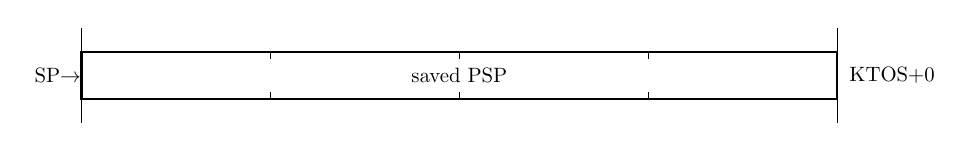
\begin{tikzpicture}[scale=0.6, every node/.style={scale=0.75}]
\draw[thick] (0,3) rectangle ++(16,1); \node at (8,3.5) {saved PSP};
\foreach \x in {4,8,12} { \draw (\x,3) -- ++(0,.15);  \draw (\x,4) -- ++(0,-.15); }
\foreach \x in {0,16} \draw (\x,2.5) -- (\x,4.5);
\node at (-.5,3.5) {SP$\rightarrow$};
\foreach \y/\offset in {3.5/0} \node[anchor=west] at (16.1,\y) {KTOS+\offset};
\end{tikzpicture}
\end{center}

Init the \lstinline{NEED_SWITCH}/\lstinline{SAVE} in \lstinline{tpl_kern}.

\begin{lstlisting}[backgroundcolor=\color{red!15}]
    mov #tpl_kern, r11
    mov.b #NO_NEED_SWITCH_NOR_SCHEDULE, TPL_KERN_OFFSET_NEED_SWITCH(r11)
    mov.b #NO_NEED_SWITCH_NOR_SCHEDULE, TPL_KERN_OFFSET_NEED_SCHEDULE(r11)
\end{lstlisting}

Call the service.

\begin{lstlisting}[backgroundcolor=\color{red!15}]
    rla  REG_SID /* index -> offset */
    call tpl_dispatch_table(REG_SID)
\end{lstlisting}

From there, \lstinline{REG_RETARG} holds the return value. It is put at its location in the process stack. Also \lstinline{r13} and \lstinline{r14} become usable whatever is the ABI.

\begin{lstlisting}[backgroundcolor=\color{red!15}]
    mov  @r1, r13           //get back PSP => r13
    mov  REG_RETARG, 8(r13) //put in Process's stack
\end{lstlisting}

Check the context switch condition in \lstinline{tpl_kern}.
\begin{lstlisting}[backgroundcolor=\color{red!15}]
    mov     #tpl_kern, r11
    tst.b   TPL_KERN_OFFSET_NEED_SWITCH(r11)
    jz      tpl_sc_handler_no_context_switch
\end{lstlisting}

Prepare the call to \lstinline{tpl_run_elected} by setting \lstinline{REG_RETARG} to 0, aka no save.
\begin{lstlisting}[backgroundcolor=\color{red!15}]
    mov     #0, REG_RETARG
\end{lstlisting}

Test the \lstinline{NEED_SAVE} condition.

\begin{lstlisting}[backgroundcolor=\color{red!15}]
    bit.b   #NEED_SAVE, TPL_KERN_OFFSET_NEED_SWITCH(r11)
    jz      tpl_sc_handler_no_save_running_context
\end{lstlisting}
Save the context. The MSP430 have a ``push multiple words", but no ``move multiple word". So, we get back to process stack to benefit this instruction

\begin{lstlisting}[backgroundcolor=\color{red!15}]
    mov     r1, r14	/* get a copy of the KSP to restore it later */
\end{lstlisting}
\begin{lstlisting}[backgroundcolor=\color{yellow!15}]
    mov     r13, r1	/* change stack to process stack */	
    pushm.w #7, r10	/* Push r4 to r10 on process stack (save) */
\end{lstlisting}

\textbf{The stack pointer has been changed ! r13 IS NOT UP TO DATE !}

\begin{lstlisting}[backgroundcolor=\color{red!15}]
    mov     r14, r1	/* get back to kernel stack */
\end{lstlisting}

The whole context is now saved on process stack and the kernel stack has been cleaned. The saved context structure is shown at figure \ref{fig:context}.


\begin{figure}[h!]
\caption{Context saved on stack}
\begin{center}
\begin{tikzpicture}[xscale=0.6, yscale=-.6, every node/.style={scale=0.75}]
\foreach \r in {4,5,...,10} {
	\draw[thick] ($(0,\r-4)$) rectangle ++(16,1); \node at ($(8,\r-4+.5)$) {saved r\r};
}
\draw[thick] (0,7) rectangle ++(16,1); \node at (8,7.5) {saved r11};
\draw[thick] (0,13) rectangle ++(16,1); \node at (8,13.5) {saved PC};
\foreach \x in {4,8,12} { \draw (\x,13) -- ++(0,.15);  \draw (\x,14) -- ++(0,-.15); }
\draw[thick] (0,12) rectangle ++(16,1); \node at (2,12.5) {0 0 0 0}; \node at (10,12.5) {saved SR};
\foreach \x in {8,12} { \draw (\x,12) -- ++(0,.15);  \draw (\x,13) -- ++(0,-.15); }
\draw (4,12) -- ++(0,1);
\foreach \y in {8,9,10} {
	\draw[thick] (0,\y) rectangle ++(16,1); \node at ($(8,\y+.5)$) {space of arg};
}
\draw[thick] (0,11) rectangle ++(16,1); \node at ($(8,11.5)$) {{\small REG\_RETARG}};
\foreach \x in {0,16} \draw (\x,-.5) -- (\x,14.5);
\node at (-.5,0.5) {SP$\rightarrow$};
\foreach \offset in {0,2,...,26} \node[anchor=west] at ($(16.1,.5+.5*\offset)$) {PTOS+\offset};
\end{tikzpicture}
\end{center}
\label{fig:context}
\end{figure}

Now the stack pointer is saved in the dedicated location.

\begin{lstlisting}[backgroundcolor=\color{red!15}]
    mov     &tpl_kern, r11  /* Get the s_running slot of tpl_kern in r11 */
    mov     @r11, r11       /* Get the pointer to the context (SP alone) */
    mov     r13, @r11       /* Save the stack pointer                    */
\end{lstlisting}

\textbf{HERE r13 IS THE OLD STACK POINTER !}

Prepare the argument of \lstinline{tpl_run_elected} : 1 (aka save) and call it after switching back to the kernel stack.

\begin{lstlisting}[backgroundcolor=\color{red!15}]
    mov     #1, REG_RETARG
tpl_sc_handler_no_save_running_context:
    call    tpl_run_elected
\end{lstlisting}

\lstinline{tpl_run_elected} has copied the elected process slot of \lstinline{tpl_kern} to the \lstinline{running} slot. We load the stack pointer of the new running process.

\begin{lstlisting}[backgroundcolor=\color{red!15}]
    mov     &tpl_kern, r11  /* Get the s_running slot of tpl_kern in r11 */
    mov     @r11, r11       /* Get the pointer to the context (SP alone) */
\end{lstlisting}
\begin{lstlisting}[backgroundcolor=\color{yellow!15}]
    mov     @r11, r1        /* Get the stack pointer                     */
\end{lstlisting}

Now, the context of the new running process is loaded. At start it has the same pattern as the one shown at figure \ref{fig:context}. First we pop \lstinline{r4} to \lstinline{r10}

\begin{lstlisting}[backgroundcolor=\color{yellow!15}]
    popm.w #7,r10       /* Pop r4 to r10  */
    jmp    tpl_sc_end_of_context_switch
\end{lstlisting}

The process stack is then as in figure \ref{fig:stackShapeBeforeCallingService}.

%\begin{figure}[h!]
%\caption{Process stack just loaded}
%\begin{center}
%\begin{tikzpicture}[scale=0.6, every node/.style={scale=0.75}]
%%\draw[thick] (0,7) rectangle ++(16,1); \node at (8,7.5) {saved r10 [15..0]};
%%\foreach \x in {4,8,12} { \draw (\x,7) -- ++(0,.15);  \draw (\x,8) -- ++(0,-.15); }
%%\draw[thick] (0,6) rectangle ++(16,1); \node at (14,6.5) {saved r10 [19..16]};
%%\draw[pattern=north west lines, pattern color=purple] (0,6) rectangle ++(12,1);
%\draw[thick] (0,13) rectangle ++(16,1); \node at (8,13.5) {saved r11 [15..0]};
%\foreach \x in {4,8,12} { \draw (\x,13) -- ++(0,.15);  \draw (\x,14) -- ++(0,-.15); }
%\draw[thick] (0,12) rectangle ++(16,1); \node at (14,12.5) {saved r11 [19..16]};
%\draw[pattern=north west lines, pattern color=purple] (0,12) rectangle ++(12,1);
%%\draw[thick] (0,3) rectangle ++(16,1); \node at (8,3.5) {saved PC [15..0]};
%%\foreach \x in {4,8,12} { \draw (\x,3) -- ++(0,.15);  \draw (\x,4) -- ++(0,-.15); }
%%\draw[thick] (0,2) rectangle ++(16,1); \node at (14,2.5) {saved PC [19..16]};
%%\draw[pattern=north west lines, pattern color=purple] (0,2) rectangle ++(12,1);
%
%\draw[thick] (0,2) rectangle ++(16,1); \node at (8,2.5) {saved PC [15..0]};
%\foreach \x in {4,8,12} { \draw (\x,3) -- ++(0,.15);  \draw (\x,4) -- ++(0,-.15); }
%\draw[thick] (0,3) rectangle ++(16,1); \node at (2,3.5) {saved PC [19..16]};
%\draw[thick] (0,3) rectangle ++(16,1); \node at (10,3.5) {saved SR [11..0]};
%\foreach \x in {4,8,12} { \draw (\x,2) -- ++(0,.15);  \draw (\x,3) -- ++(0,-.15); }
%\draw (4,3) -- ++(0,1);
%
%
%%\draw[thick] (0,1) rectangle ++(16,1); \node at (8,1.5) {service identifier};
%%\foreach \x in {4,8,12} { \draw (\x,1) -- ++(0,.15);  \draw (\x,2) -- ++(0,-.15); }
%%\draw[thick] (0,0) rectangle ++(16,1); \node at (14,.5) {saved r11 [19..16]};
%%\draw (12,0) -- ++(0,1);
%%\draw[pattern=north west lines, pattern color=purple] (0,0) rectangle ++(12,1);
%
%\foreach \y in {6,7,...,11} {
%\draw[thick] (0,\y) rectangle ++(16,1); \node at ($(8,\y+.5)$) {space of arg};
%\foreach \x in {4,8,12} { \draw (\x,\y) -- ++(0,.15);  \draw ($(\x,\y+1)$) -- ++(0,-.15); }
%}
%
%\draw[thick] (0,5) rectangle ++(16,1); \node at ($(8,5.5)$) {\small REG\_RETARG [15..0]};
%\foreach \x in {4,8,12} { \draw (\x,5) -- ++(0,.15);  \draw ($(\x,6)$) -- ++(0,-.15); }
%\draw[thick] (0,4) rectangle ++(16,1); \node at ($(14,4.5)$) {\scriptsize REG\_RETARG [19..16]};
%\draw[pattern=north west lines, pattern color=purple] (0,4) rectangle ++(12,1);
%
%\foreach \x in {0,16} \draw (\x,1.5) -- (\x,14.5);
%\node at (-.5,13.5) {SP$\rightarrow$};
%\foreach \offset in {0,2,...,22} \node[anchor=west] at ($(16.1,13.5-.5*\offset)$) {PTOS+\offset};
%\end{tikzpicture}
%\end{center}
%\label{fig:processStackLoaded}
%\end{figure}

In case of no context switch, we have to get to the process stack, stored in r13

\begin{lstlisting}[backgroundcolor=\color{red!15}]
tpl_sc_handler_no_context_switch:
    mov r13, r1	 /* get back to process stack */
\end{lstlisting}
At last the reentrancy counter is decremented, r11 is restored, the \emph{space of args}, used in asynchronous preemption is removed from stack and the \lstinline{REG_RETARG} is poped.

Interrupts are enables during the \texttt{reti} instruction because it is related to the \texttt{GIE} bit in the status register.
\begin{lstlisting}[backgroundcolor=\color{yellow!15}]
tpl_sc_end_of_context_switch:
    dec.b  &tpl_reentrancy_counter
    jnz    tpl_sc_handler_still_in_kernel    

tpl_sc_handler_still_in_kernel:
    popx.w r11
    add    #12,r1       /* Skip volatile             */
    popx.w REG_RETARG   /* Get back the return value */
    reti
\end{lstlisting}

\textbf{Here instead of a add, a pop should be done because this context may have been pushed under interrupts !}

\subsection{Context initialisation}
The context that shoud be set during the task's initialisation (\texttt{tpl\_init\_context}) is the one of the figure \ref{fig:context}, but with a call to either \texttt{CallTerminateTask} or \texttt{CallTerminateISR2}, depending of the type of the process to init.

\emph{TODO} Works only with 16-bit register.Should be updated.

\begin{figure}[h!]
\caption{Context initialisation}
\begin{center}
\begin{tikzpicture}[xscale=0.6, yscale=-.6, every node/.style={scale=0.75}]
\foreach \r in {4,5,...,10} {
	\draw[thick] ($(0,\r-4)$) rectangle ++(16,1); \node at ($(8,\r-4+.5)$) {saved r\r};
}
\draw[thick] (0,7) rectangle ++(16,1); \node at (8,7.5) {saved r11};
\draw[thick] (0,13) rectangle ++(16,1); \node at (8,13.5) {saved PC [15..0]};
\foreach \x in {4,8,12} { \draw (\x,13) -- ++(0,.15);  \draw (\x,14) -- ++(0,-.15); }
\draw[thick] (0,12) rectangle ++(16,1); \node at (2,12.5) {saved PC [19..16]}; \node at (10,12.5) {saved SR [11..0]};
\foreach \x in {8,12} { \draw (\x,12) -- ++(0,.15);  \draw (\x,13) -- ++(0,-.15); }
\draw (4,12) -- ++(0,1);
\foreach \y in {8,9,10} {
	\draw[thick] (0,\y) rectangle ++(16,1); \node at ($(8,\y+.5)$) {space of arg};
}
\draw[thick] (0,11) rectangle ++(16,1); \node at ($(8,11.5)$) {{\small REG\_RETARG}};
\draw[thick] (0,14) rectangle ++(16,1); \node at (8,14.5) {CallTerminateXXX [15..0]};
%\foreach \x in {4,8,12} { \draw (\x,1) -- ++(0,.15);  \draw (\x,2) -- ++(0,-.15); }
\foreach \x in {0,16} \draw (\x,-.5) -- (\x,15.5);
\node at (-.5,0.5) {SP$\rightarrow$};
\foreach \offset in {0,2,...,28} \node[anchor=west] at ($(16.1,.5+.5*\offset)$) {PTOS+\offset};
\end{tikzpicture}


%\begin{tikzpicture}[scale=0.55, every node/.style={scale=0.75}]
%
%\foreach \reg/\y in {10/7,9/9,8/11,7/13,6/15,5/17,4/19} {
%\draw[thick] ($(0,\y+8)$) rectangle ++(16,1); \node at ($(8,\y+8.5)$) {saved r\reg [15..0]};
%\foreach \x in {4,8,12} { \draw ($(\x,\y+8)$) -- ++(0,.15);  \draw ($(\x,\y+9)$) -- ++(0,-.15); }
%\draw[thick] ($(0,\y+7)$) rectangle ++(16,1); \node at ($(14,\y+7.5)$) {saved r\reg [19..16]};
%\draw[pattern=north west lines, pattern color=purple] ($(0,\y+7)$) rectangle ++(12,1);
%}
%
%\draw[thick] (0,5) rectangle ++(16,1); \node at (8,5.5) {\small REG\_RETARG [15..0]};
%\foreach \x in {4,8,12} { \draw (\x,23) -- ++(0,.15);  \draw (\x,5) -- ++(0,-.15); }
%\draw[thick] (0,4) rectangle ++(16,1); \node at (14,4.5) {\scriptsize REG\_RETARG [19..16]};
%\draw[pattern=north west lines, pattern color=purple] (0,4) rectangle ++(12,1);
%
%
%\foreach \y in {6,7,...,11} {
%\draw[thick] (0,\y) rectangle ++(16,1); \node at ($(8,\y+.5)$) {space of arg};
%}
%
%%\draw[thick] (0,6) rectangle ++(16,1); \node at (8,6.5) {saved r15};
%%\foreach \x in {4,8,12} { \draw (\x,6) -- ++(0,.15);  \draw (\x,7) -- ++(0,-.15); }
%
%\draw[thick] (0,13) rectangle ++(16,1); \node at (8,13.5) {saved r11 [15..0]};
%\foreach \x in {4,8,12} { \draw (\x,5) -- ++(0,.15);  \draw (\x,6) -- ++(0,-.15); }
%\draw[thick] (0,12) rectangle ++(16,1); \node at (14,12.5) {saved r11 [19..16]};
%\draw[pattern=north west lines, pattern color=purple] (0,12) rectangle ++(12,1);
%
%\draw[thick] (0,2) rectangle ++(16,1); \node at (8,2.5) {saved PC [15..0]};
%\foreach \x in {4,8,12} { \draw (\x,3) -- ++(0,.15);  \draw (\x,4) -- ++(0,-.15); }
%\draw[thick] (0,3) rectangle ++(16,1); \node at (2,3.5) {saved PC [19..16]};
%\draw[thick] (0,3) rectangle ++(16,1); \node at (10,3.5) {saved SR [11..0]};
%\foreach \x in {4,8,12} { \draw (\x,2) -- ++(0,.15);  \draw (\x,3) -- ++(0,-.15); }
%\draw (4,3) -- ++(0,1);
%\foreach \x in {0,16} \draw (\x,1.5) -- (\x,28.5);
%\node at (-.5,27.5) {SP$\rightarrow$};
%\foreach \offset in {0,2,...,52} \node[anchor=west] at ($(16.1,27.5-.5*\offset)$) {PTOS+\offset};
%%22.5/0,21.5/2,20.5/4,19.5/6,18.5/8,17.5/10,16.5/12,15.5/14,14.5/16,13.5/18,
%%12.5/20,11.5/22,10.5/24,9.5/26,8.5/28,7.5/30,6.5/32,5.5/34,4.5/36,3.5/38,2.5/40,
%%1.5/42,0.5/44,-.5/46,-1.5/48,-2.5/50,-3.5/52,-4.5/54
%%} \node[anchor=west] at ($(16.1,\y+7)$) {PTOS+\offset};
%\draw[thick] (0,1) rectangle ++(16,1); \node at (8,1.5) {CallTerminateXXX [15..0]};
%\foreach \x in {4,8,12} { \draw (\x,1) -- ++(0,.15);  \draw (\x,2) -- ++(0,-.15); }
%\end{tikzpicture}
\end{center}
\label{fig:contextInit}
\end{figure}


\section{The Systick Handler}

The Systick is generated by using a \lstinline{TIMERA} register. On the MSP430FR5969, \lstinline{TIMERA3} has been chosen. When entering the ISR, the stack is as shown at figure \ref{fig:stackit} and \lstinline{PC} (\lstinline{r0}) and \lstinline{SR} (\lstinline{r2}) have been saved. Before doing anything we have to save the volatile registers, which are \lstinline{r11}\footnote{r11 is not volatile in the \emph{MSPGCC} ABI but is volatile in \emph{GCC compiler for MSP} ABI. Anyway, in order to limit variabilility, \lstinline{r11} is saved for both ABIs.} to \lstinline{r15}, because they will not be saved when we will call the \lstinline{tpl_counter_tick_SystemCounter} C function.

\begin{lstlisting}[basicstyle=\footnotesize\ttfamily]
tpl_systick_handler:
    pushx.a REG_RETARG
#ifdef MSPGCC_ABI
    /* r15 has been pushed by pushx.a REG_RETARG */
    pushm.a #4, r14  /* Push r11, r12, r13, r14 */
#endif
#ifdef GCCFORMSP_ABI
    /* r12 has been pushed by pushx.a REG_RETARG */
    pushm.a #3, r15  /* Push r13, r14, r15 */
    pushx.a r11
#endif
\end{lstlisting}

As a result the stack is as follow for \emph{MSPGCC} ABI:

\begin{center}
\begin{tikzpicture}[scale=0.6, every node/.style={scale=0.75}]
%\draw[thick] (0,7) rectangle ++(16,1); \node at (8,7.5) {saved r10 [15..0]};
%\foreach \x in {4,8,12} { \draw (\x,7) -- ++(0,.15);  \draw (\x,8) -- ++(0,-.15); }
%\draw[thick] (0,6) rectangle ++(16,1); \node at (14,6.5) {saved r10 [19..16]};
%\draw[pattern=north west lines, pattern color=purple] (0,6) rectangle ++(12,1);
%\draw[thick] (0,13) rectangle ++(16,1); \node at (8,13.5) {saved r11 [15..0]};
%\foreach \x in {4,8,12} { \draw (\x,13) -- ++(0,.15);  \draw (\x,14) -- ++(0,-.15); }
%\draw[thick] (0,12) rectangle ++(16,1); \node at (14,12.5) {saved r11 [19..16]};
%\draw[pattern=north west lines, pattern color=purple] (0,12) rectangle ++(12,1);
%\draw[thick] (0,3) rectangle ++(16,1); \node at (8,3.5) {saved PC [15..0]};
%\foreach \x in {4,8,12} { \draw (\x,3) -- ++(0,.15);  \draw (\x,4) -- ++(0,-.15); }
%\draw[thick] (0,2) rectangle ++(16,1); \node at (14,2.5) {saved PC [19..16]};
%\draw[pattern=north west lines, pattern color=purple] (0,2) rectangle ++(12,1);

\draw[thick] (0,2) rectangle ++(16,1); \node at (8,2.5) {saved PC [15..0]};
\foreach \x in {4,8,12} { \draw (\x,3) -- ++(0,.15);  \draw (\x,4) -- ++(0,-.15); }
\draw[thick] (0,3) rectangle ++(16,1); \node at (2,3.5) {saved PC [19..16]};
\draw[thick] (0,3) rectangle ++(16,1); \node at (10,3.5) {saved SR [11..0]};
\foreach \x in {4,8,12} { \draw (\x,2) -- ++(0,.15);  \draw (\x,3) -- ++(0,-.15); }
\draw (4,3) -- ++(0,1);


%\draw[thick] (0,1) rectangle ++(16,1); \node at (8,1.5) {service identifier};
%\foreach \x in {4,8,12} { \draw (\x,1) -- ++(0,.15);  \draw (\x,2) -- ++(0,-.15); }
%\draw[thick] (0,0) rectangle ++(16,1); \node at (14,.5) {saved r11 [19..16]};
%\draw (12,0) -- ++(0,1);
%\draw[pattern=north west lines, pattern color=purple] (0,0) rectangle ++(12,1);

%\foreach \y in {6,7,...,11} {
%\draw[thick] (0,\y) rectangle ++(16,1); \node at ($(8,\y+.5)$) {space of arg};
%\foreach \x in {4,8,12} { \draw (\x,\y) -- ++(0,.15);  \draw ($(\x,\y+1)$) -- ++(0,-.15); }
%}
\foreach \reg in {11,12,13,14} {
\draw[thick] ($(0,35-2*\reg)$) rectangle ++(16,1); \node at ($(8,35.5-2*\reg)$) {saved r\reg [15..0]};
\foreach \x in {4,8,12} { \draw ($(\x,35-2*\reg)$) -- ++(0,.15);  \draw ($(\x,36-2*\reg)$) -- ++(0,-.15); }
\draw[thick] ($(0,34-2*\reg)$) rectangle ++(16,1); \node at ($(14,34.5-2*\reg)$) {saved r\reg [19..16]};
\draw[pattern=north west lines, pattern color=purple] ($(0,34-2*\reg)$) rectangle ++(12,1);
}

\draw[thick] (0,5) rectangle ++(16,1); \node at ($(8,5.5)$) {{\small REG\_RETARG} [15..0] aka r15};
\foreach \x in {4,8,12} { \draw (\x,5) -- ++(0,.15);  \draw ($(\x,6)$) -- ++(0,-.15); }
\draw[thick] (0,4) rectangle ++(16,1); \node at ($(14,4.5)$) {\scriptsize REG\_RETARG [19..16]};
\draw[pattern=north west lines, pattern color=purple] (0,4) rectangle ++(12,1);

\foreach \x in {0,16} \draw (\x,1.5) -- (\x,14.5);
\node at (-.5,13.5) {SP$\rightarrow$};
\foreach \offset in {0,2,...,22} \node[anchor=west] at ($(16.1,13.5-.5*\offset)$) {PTOS+\offset};
\end{tikzpicture}
\end{center}
%\begin{center}
%\begin{tikzpicture}[scale=0.7, every node/.style={scale=0.75}]
%
%%\foreach \reg/\y in {15/} {
%%\draw[thick] (0,5) rectangle ++(16,1); \node at (8,5.5) {saved r11 [15..0]};
%%\foreach \x in {4,8,12} { \draw (\x,5) -- ++(0,.15);  \draw (\x,6) -- ++(0,-.15); }
%%\draw[thick] (0,4) rectangle ++(16,1); \node at (14,4.5) {saved r11 [19..16]};
%%\draw[pattern=north west lines, pattern color=purple] (0,4) rectangle ++(12,1);
%%}
%
%\draw[thick] (0,2) rectangle ++(16,1); \node at (8,2.5) {saved PC [15..0]};
%\foreach \x in {4,8,12} { \draw (\x,3) -- ++(0,.15);  \draw (\x,4) -- ++(0,-.15); }
%\draw[thick] (0,3) rectangle ++(16,1); \node at (2,3.5) {saved PC [19..16]};
%\draw[thick] (0,3) rectangle ++(16,1); \node at (10,3.5) {saved SR [11..0]};
%\foreach \x in {4,8,12} { \draw (\x,2) -- ++(0,.15);  \draw (\x,3) -- ++(0,-.15); }
%\draw (4,3) -- ++(0,1);
%\foreach \x in {0,16} \draw (\x,1.5) -- (\x,6.5);
%\node at (-.5,5.5) {SP$\rightarrow$};
%\foreach \y/\offset in {5.5/0,4.5/2,3.5/4,2.5/6} \node at (17,\y) {PTOS+\offset};
%\end{tikzpicture}
%\end{center}

And as follow for the \emph{GCC compiler for MSP} ABI:

\begin{center}
\begin{tikzpicture}[scale=0.6, every node/.style={scale=0.75}]
%\draw[thick] (0,7) rectangle ++(16,1); \node at (8,7.5) {saved r10 [15..0]};
%\foreach \x in {4,8,12} { \draw (\x,7) -- ++(0,.15);  \draw (\x,8) -- ++(0,-.15); }
%\draw[thick] (0,6) rectangle ++(16,1); \node at (14,6.5) {saved r10 [19..16]};
%\draw[pattern=north west lines, pattern color=purple] (0,6) rectangle ++(12,1);
\draw[thick] (0,13) rectangle ++(16,1); \node at (8,13.5) {saved r11 [15..0]};
\foreach \x in {4,8,12} { \draw (\x,13) -- ++(0,.15);  \draw (\x,14) -- ++(0,-.15); }
\draw[thick] (0,12) rectangle ++(16,1); \node at (14,12.5) {saved r11 [19..16]};
\draw[pattern=north west lines, pattern color=purple] (0,12) rectangle ++(12,1);
%\draw[thick] (0,3) rectangle ++(16,1); \node at (8,3.5) {saved PC [15..0]};
%\foreach \x in {4,8,12} { \draw (\x,3) -- ++(0,.15);  \draw (\x,4) -- ++(0,-.15); }
%\draw[thick] (0,2) rectangle ++(16,1); \node at (14,2.5) {saved PC [19..16]};
%\draw[pattern=north west lines, pattern color=purple] (0,2) rectangle ++(12,1);

\draw[thick] (0,2) rectangle ++(16,1); \node at (8,2.5) {saved PC [15..0]};
\foreach \x in {4,8,12} { \draw (\x,3) -- ++(0,.15);  \draw (\x,4) -- ++(0,-.15); }
\draw[thick] (0,3) rectangle ++(16,1); \node at (2,3.5) {saved PC [19..16]};
\draw[thick] (0,3) rectangle ++(16,1); \node at (10,3.5) {saved SR [11..0]};
\foreach \x in {4,8,12} { \draw (\x,2) -- ++(0,.15);  \draw (\x,3) -- ++(0,-.15); }
\draw (4,3) -- ++(0,1);


%\draw[thick] (0,1) rectangle ++(16,1); \node at (8,1.5) {service identifier};
%\foreach \x in {4,8,12} { \draw (\x,1) -- ++(0,.15);  \draw (\x,2) -- ++(0,-.15); }
%\draw[thick] (0,0) rectangle ++(16,1); \node at (14,.5) {saved r11 [19..16]};
%\draw (12,0) -- ++(0,1);
%\draw[pattern=north west lines, pattern color=purple] (0,0) rectangle ++(12,1);

%\foreach \y in {6,7,...,11} {
%\draw[thick] (0,\y) rectangle ++(16,1); \node at ($(8,\y+.5)$) {space of arg};
%\foreach \x in {4,8,12} { \draw (\x,\y) -- ++(0,.15);  \draw ($(\x,\y+1)$) -- ++(0,-.15); }
%}
\foreach \reg in {13,14,15} {
\draw[thick] ($(0,37-2*\reg)$) rectangle ++(16,1); \node at ($(8,37.5-2*\reg)$) {saved r\reg [15..0]};
\foreach \x in {4,8,12} { \draw ($(\x,37-2*\reg)$) -- ++(0,.15);  \draw ($(\x,38-2*\reg)$) -- ++(0,-.15); }
\draw[thick] ($(0,36-2*\reg)$) rectangle ++(16,1); \node at ($(14,36.5-2*\reg)$) {saved r\reg [19..16]};
\draw[pattern=north west lines, pattern color=purple] ($(0,36-2*\reg)$) rectangle ++(12,1);
}

\draw[thick] (0,5) rectangle ++(16,1); \node at ($(8,5.5)$) {{\small REG\_RETARG} [15..0] aka r12};
\foreach \x in {4,8,12} { \draw (\x,5) -- ++(0,.15);  \draw ($(\x,6)$) -- ++(0,-.15); }
\draw[thick] (0,4) rectangle ++(16,1); \node at ($(14,4.5)$) {\scriptsize REG\_RETARG [19..16]};
\draw[pattern=north west lines, pattern color=purple] (0,4) rectangle ++(12,1);

\foreach \x in {0,16} \draw (\x,1.5) -- (\x,14.5);
\node at (-.5,13.5) {SP$\rightarrow$};
\foreach \offset in {0,2,...,22} \node[anchor=west] at ($(16.1,13.5-.5*\offset)$) {PTOS+\offset};
\end{tikzpicture}
\end{center}

Switch to the kernel stack.

\begin{lstlisting}[basicstyle=\footnotesize\ttfamily]
    mov r1,r11                     /* Copy the PSP in r11        */
    mov #tpl_kern_stack_bottom, r1 /* Switch to the kernel stack */
    push r11                       /* Save PCP to kernel stack   */
\end{lstlisting}

The kernel stack is as follow:

\begin{center}
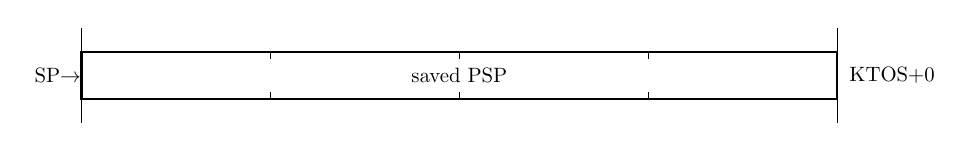
\begin{tikzpicture}[scale=0.6, every node/.style={scale=0.75}]
%\draw[thick] (0,7) rectangle ++(16,1); \node at (8,7.5) {saved r10 [15..0]};
%\foreach \x in {4,8,12} { \draw (\x,7) -- ++(0,.15);  \draw (\x,8) -- ++(0,-.15); }
%\draw[thick] (0,6) rectangle ++(16,1); \node at (14,6.5) {saved r10 [19..16]};
%\draw[pattern=north west lines, pattern color=purple] (0,6) rectangle ++(12,1);
%\draw[thick] (0,5) rectangle ++(16,1); \node at (8,5.5) {saved r11 [15..0]};
%\foreach \x in {4,8,12} { \draw (\x,5) -- ++(0,.15);  \draw (\x,6) -- ++(0,-.15); }
%\draw[thick] (0,4) rectangle ++(16,1); \node at (14,4.5) {saved r11 [19..16]};
%\draw[pattern=north west lines, pattern color=purple] (0,4) rectangle ++(12,1);
\draw[thick] (0,3) rectangle ++(16,1); \node at (8,3.5) {saved PSP};
\foreach \x in {4,8,12} { \draw (\x,3) -- ++(0,.15);  \draw (\x,4) -- ++(0,-.15); }
%\draw[thick] (0,2) rectangle ++(16,1); \node at (14,2.5) {saved PC [19..16]};
%\draw[pattern=north west lines, pattern color=purple] (0,2) rectangle ++(12,1);
%\draw[thick] (0,1) rectangle ++(16,1); \node at (8,1.5) {service identifier};
%\foreach \x in {4,8,12} { \draw (\x,1) -- ++(0,.15);  \draw (\x,2) -- ++(0,-.15); }
%\draw[thick] (0,0) rectangle ++(16,1); \node at (14,.5) {saved r11 [19..16]};
%\draw (12,0) -- ++(0,1);
%\draw[pattern=north west lines, pattern color=purple] (0,0) rectangle ++(12,1);
\foreach \x in {0,16} \draw (\x,2.5) -- (\x,4.5);
\node at (-.5,3.5) {SP$\rightarrow$};
\foreach \y/\offset in {3.5/0} \node[anchor=west] at (16.1,\y) {KTOS+\offset};
\end{tikzpicture}
\end{center}

Init the \lstinline{NEED_SWITCH}/\lstinline{SAVE} in \lstinline{tpl_kern}.

\begin{lstlisting}[basicstyle=\footnotesize\ttfamily]
    mov   #tpl_kern, r11
    mov.b #NO_NEED_SWITCH_NOR_SCHEDULE, TPL_KERN_OFFSET_NEED_SWITCH(r11)
    mov.b #NO_NEED_SWITCH_NOR_SCHEDULE, TPL_KERN_OFFSET_NEED_SCHEDULE(r11)
\end{lstlisting}

Call the function that increments the SystemCounter and manages alarm.

\begin{lstlisting}[basicstyle=\footnotesize\ttfamily]
    call tpl_counter_tick_SystemCounter
\end{lstlisting}

Switch back to the process stack

\begin{lstlisting}[basicstyle=\footnotesize\ttfamily]
    mov r1, r13 /* get a copy of the KSP to restore it later */
    pop r1      /* get the saved process stack pointer back  */
\end{lstlisting}

Check the context switch condition in \lstinline{tpl_kern}.

\begin{lstlisting}[basicstyle=\footnotesize\ttfamily]
    mov   #tpl_kern, r11
    tst.b TPL_KERN_OFFSET_NEED_SWITCH(r11)
    jz    tpl_systick_handler_no_context_switch
\end{lstlisting}

Save the rest of the context.

\begin{lstlisting}[basicstyle=\footnotesize\ttfamily]
    pushm.a #7, r10 /* Push r4 to r10 */
\end{lstlisting}

Now the stack pointer is saved in the dedicated location.

\begin{lstlisting}[basicstyle=\footnotesize\ttfamily]
    mov &tpl_kern, r11  /* Get the s_running slot of tpl_kern in r11 */
    mov @r11, r11       /* Get the pointer to the context (SP alone) */
    mov r1, @r11        /* Save the stack pointer                    */
\end{lstlisting}

Call \lstinline{tpl_run_elected} with argument 1 (aka save) after switching back to the kernel stack.

\begin{lstlisting}[basicstyle=\footnotesize\ttfamily]
    mov r13, r1         /* Switch back to the kernel stack         */
    mov #1, REG_RETARG
    add #2, r1          /* "pop" the PSP which is no longer useful */
    call tpl_run_elected
\end{lstlisting}

\lstinline{tpl_run_elected} has copied the elected process slot of \lstinline{tpl_kern} to the \lstinline{running} slot. We load the stack pointer of the new running process.

\begin{lstlisting}[basicstyle=\footnotesize\ttfamily]
    mov &tpl_kern, r11  /* Get the s_running slot of tpl_kern in r11 */
    mov @r11, r11       /* Get the pointer to the context (SP alone) */
    mov @r11, r1        /* Get the stack pointer                     */
\end{lstlisting}

Now, the context of the new running process is loaded. First we pop \lstinline{r4} to \lstinline{r10}

\begin{lstlisting}[basicstyle=\footnotesize\ttfamily]
    popm.a #7,r10       /* Pop r4 to r10  */
\end{lstlisting}



Restore the volatile registers and return from the interrupt handler.

\begin{lstlisting}[basicstyle=\footnotesize\ttfamily]
tpl_systick_handler_no_context_switch:

#ifdef MSPGCC_ABI
    /* r15 will be popped by popx.a REG_RETARG */
    popm.a #4, r14  /* Pop r11, r12, r13, r14 */
#endif
#ifdef GCCFORMSP_ABI
    /* r12 will be popped by popx.a REG_RETARG */
    popx.a r11
    popm.a #3, r15  /* Pop r13, r14, r15 */
#endif
    popx.a REG_RETARG
    reti
\end{lstlisting}

That's all !

\bibliographystyle{plain}
\bibliography{porting}

\end{document}  

%!TEX root = ./main.tex

\chapter{Ports details}

\section{PowerPC}

\subsection{System services} \label{sec:systemservices}

The PowerPC port uses the \asfct{sc} software interrupt to call system services \cite{mpc32bsc}. \asfct{sc} stands for System Call. It saves the current \reg{PC} in \reg{SRR0} register and the current \reg{MSR} in \reg{SRR1} register and jump to the System Call handler.

The id of the system service to call is given in the \reg{r0} register and \reg{r0} save and restore are added around. For instance, the following listing gives the \api{ActivateTask} service code. These function are generated from templates by goil (see \ref{sec:generatedfiles}) and are part of the {\em invoque} layer (see \ref{sec:invoque}):

\begin{lstlisting}[language=C]
  .global ActivateTask
ActivateTask:
  subi r1,r1,4                       /* make room on stack    */
  stw  r0,0(r1)                      /* save r0               */
  li   r0,OSServiceId_ActivateTask   /* load r0 with the id   */
  sc                                 /* system call           */
  lwz  r0,0(r1)                      /* restore r0            */
  addi r1,r1,4                       /* restore stack         */
  blr                                /* return                */
  
  .type ActivateTask,@function
  .size ActivateTask,$$-ActivateTask
\end{lstlisting}

When the System Call begin execution, the process stack has the mapping depicted in figure \ref{fig:stackbeginningSC}.

\begin{figure}[htbp] %  figure placement: here, top, bottom, or page
\begin{minipage}{0.5\textwidth}
    \centering
  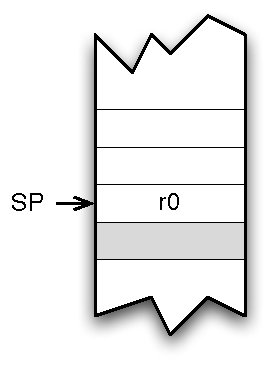
\includegraphics[scale=.6]{pictures/PStackAfterInvoque} 
\end{minipage}
\begin{minipage}{0.5\textwidth}
   \caption{Process stack mapping at the beginning of the System Call handler. The grayed zone represents an unknown content depending on from where the service was called.}\label{fig:stackbeginningSC}
\end{minipage}
\end{figure}

\subsection{Dispatching the service call}

The System Call handler is usually located in the \hex{0C00} exception handler but, depending on the CPU kind, it may be located elsewhere. Since the available memory for the interrupt or exception handler may vary, a jump is made to the \cfunction{tpl_sc_handler}.%:

%\begin{lstlisting}
%  .section  .SC_vector  CODE_ACCESS_RIGHT
%tpl_sc_vector:
%  b   tpl_sc_handler
%
%  .section  .SC_handler CODE_ACCESS_RIGHT
%\end{lstlisting}

\cfunction{tpl_sc_handler} performs the following tasks:
\begin{penum}
\item saves additional registers to be able to work
\item disables memory protection
\item switches to kernel stack if needed
\item calls the service
\item performs a context switch if needed and programs the MPU.
\item switches back to the process stack if needed
\item enable memory protection
\item restore registers
\item get back to the process
\end{penum}

\note{Currently the PowerPC port does not support tasks that use floating point registers}

\subsubsection{Saving additional registers}

The following registers are saved: \var{lr}, \var{cr}, \var{r11} and \var{r12}. In fact, it should be not necessary to save \var{r11} and \var{r12} because these registers are volatile as defined in the PowerPC EABI \cite{PPCeabi} but we prefer a conservative approach. Register saving is done by the following code at start of the \cfunction{tpl_sc_handler} and the mapping of the process stack is depicted at figure \ref{fig:stackSavingSC}:

\begin{lstlisting}[language=C]
  subi  r1,r1,PS_FOOTPRINT  /* Make room on stack */

  stw   r11,PS_R11(r1)      /* Save r11           */
  stw   r12,PS_R12(r1)      /* Save r12           */
  mflr  r11
  stw   r11,PS_LR(r1)       /* Save lr            */
  mfcr  r11
  stw   r11,PS_CR(r1)       /* Save cr            */
\end{lstlisting}

\begin{figure}[htbp] %  figure placement: here, top, bottom, or page
\begin{minipage}{0.5\textwidth}
    \centering
  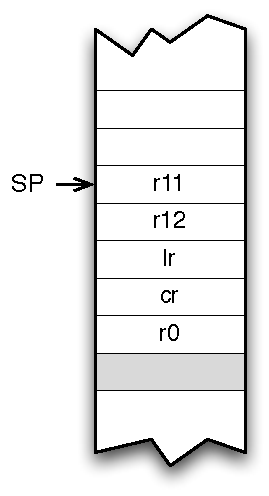
\includegraphics[scale=.6]{pictures/PStackAfterSCSaving} 
\end{minipage}
\begin{minipage}{0.5\textwidth}
   \caption{Process stack mapping after additional registers have been saved by the beginning of the System Call handler.}\label{fig:stackSavingSC}
\end{minipage}
\end{figure}

\subsubsection{Disabling memory protection}

This part of the dispatch layer is done in the \cfunction{tpl_enter_kernel} function and is assembled only if \cmacro{WITH_MEMORY_PROTECTION} is set to \YES. After saving the \reg{lr}, the \cfunction{tpl_kernel_mp} function is called and does the actual job. At last \reg{lr} is restored.

\begin{lstlisting}[language=C]
#if WITH_MEMORY_PROTECTION == YES
  /*
   * Switch to kernel mem protection scheme
   */
  subi  r1,r1,4
  mflr  r11
  stw   r11,0(r1)       /* save lr on the current stack */
  bl    tpl_kernel_mp   /* disable memory protection    */
  lwz   r11,0(r1)       /* restore lr                   */
  mtlr  r11
  addi  r1,r1,4
#endif
\end{lstlisting}

\subsubsection{Switching to the kernel stack}

Once the dispatch layer has saved the registers it uses and has switched to the kernel memory protection scheme, it switches to the kernel stack. However the kernel stack could used already because a call to a \cfunction{PreTaskHook} or a \cfunction{PostTaskHook} is done on the kernel stack and such a hook may call a service. So the dispatch layer is reentrant. The number of reentrant calls is counted by the \var{tpl_reentrancy_counter}. In addition the process stack pointer (\reg{r1}), \reg{SRR0} and \reg{SRR1} are saved in the kernel stack. The kernel stack mapping is shown in figure \ref{fig:kernelstackmapping}. For a reentrant call, the same frame is build over the current one. The switch to the kernel stack is done as follow:

\begin{lstlisting}[language=C]
  /*
   * Check the reentrency counter value and increment it
   * if the value is 0 before the inc, then we switch to
   * the system stack.
   */
  lis   r11,TPL_HIG(tpl_reentrancy_counter)
  ori   r11,r11,TPL_LOW(tpl_reentrancy_counter)
  lwz   r12,0(r11)    /* get the value of the counter */
  cmpwi r12,0
  addi  r12,r12,1
  stw   r12,0(r11)
  bne   no_stack_change
  
  /*
   * Switch to the kernel stack
   *
   * Get the pointer to the bottom of the stack
   */  
  lis   r11,TPL_HIG(tpl_kernel_stack_bottom)
  ori   r11,r11,TPL_LOW(tpl_kernel_stack_bottom)
  stw   r1,KS_SP-KS_FOOTPRINT(r11)  /* save the sp of the caller */
  mr    r1,r11                      /* set the kernel stack      */
  
no_stack_change:
  /*
   * make space on the stack to call C functions
   */
  subi  r1,r1,KS_FOOTPRINT
\end{lstlisting}

\begin{figure}[htbp] %  figure placement: here, top, bottom, or page
\begin{minipage}{0.5\textwidth}
    \centering
  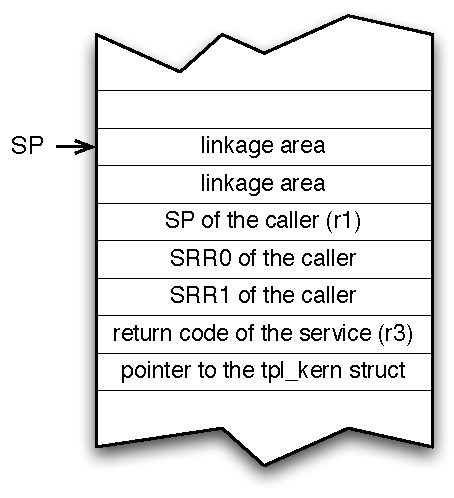
\includegraphics[scale=.6]{pictures/KStackMapping} 
\end{minipage}
\begin{minipage}{0.5\textwidth}
  \caption{Kernel stack mapping after allocation.}\label{fig:kernelstackmapping}
\end{minipage}
\end{figure}

\subsubsection{Calling the service}

Since the registers used to pass parameters to a function, that is \reg{r3} to \reg{r10} as documented in \cite{PPCeabi}, have not been changed until now, calling the function that implements the service respects the register usage conventions.

The first thing to do is to get the function pointer corresponding to the service id. The service id is in \reg{r0} as explained in \ref{sec:systemservices} and is used as an index to the \var{tpl_dispatch_table}.

\begin{lstlisting}[language=C]
  slwi  r0,r0,2                           /* compute the offset    */
  /*
   * load the ptr to the dispatch table
   */
  lis   r11,TPL_HIG(tpl_dispatch_table)     
  ori   r11,r11,TPL_LOW(tpl_dispatch_table)
  lwzx  r11,r11,r0                  /* get the ptr to the service  */
  mtlr  r11                         /* put it in lr for future use */
\end{lstlisting}

The second thing to do is to reset the \var{tpl_need_switch} flag that triggers a context switch. This flag (a byte) is located in the \var{tpl_kern} kernel struct. This is done as follow:

\begin{lstlisting}[language=C]
  lis   r11,TPL_HIG(tpl_kern)
  ori   r11,r11,TPL_LOW(tpl_kern)
  stw   r11,KS_KERN_PTR(r1)        /* save the ptr for future use  */
  li    r0,NO_NEED_SWITCH
  stb   r0,20(r11)
\end{lstlisting}

In the future \var{tpl_kern} will be reused, so its address is saved in the kernel stack.

Then, to allow reentrancy for a service call in a hook, the \reg{RI} bit of the \reg{MSR} is set to 1. Without that, a \asfct{sc} cannot be  properly executed.

\begin{lstlisting}[language=C]
  mfmsr r11
  ori   r11,r11,RI_BIT_1
  mtmsr r11
\end{lstlisting}

At last, the service is called:

\begin{lstlisting}[language=C]
  blrl
\end{lstlisting}

\subsubsection{Context switch}

The \var{tpl_need_switch} flag that as been possibly modified by the service is now checked to do a context switch if needed.

\begin{lstlisting}[language=C]
  lwz   r11,KS_KERN_PTR(r1) /* get back the tpl_kern address */
  lbz   r12,20(r11)         /* get the tpl_need_switch flag  */
  andi. r0,r12,NEED_SWITCH  /* check if a switch is needed   */
  beq   no_context_switch
\end{lstlisting}

A context switch is performed in 3 steps. The first one is the context save of the process that loses the CPU. This step is optional because if the service was a \api{TerminateTask} or a \api{ChainTask}, the context needs not to be saved. This information is in the \var{tpl_need_switch} flag. Before doing the actual context save, the return value of the service must be saved in the proper location of the kernel stack. The \cfunction{tpl_save_context} function will read it from this location and expects a pointer to the context saving area or the process in \reg{r3}. \var{s_old}, the address of the context saving area, is in another member of \var{tpl_kern}. At the end, the \var{tpl_kern} address is reread because \reg{r11} has been destroyed in \cfunction{tpl_save_context}. 

\begin{lstlisting}[language=C]
  stw   r3,KS_RETURN_CODE(r1) /* save the return value             */
  andi. r0,r12,NEED_SAVE      /* r12 contains tpl_need_switch      */
  beq   no_save
  lwz   r3,0(r11)             /* r11 contains the tpl_kern address */
  bl    tpl_save_context      /* and s_old is put into r3          */
  lwz   r11,KS_KERN_PTR(r1)   /* get back tpl_kern address         */
\end{lstlisting}

The second step consists in loading the configuration of memory protection for the process that get the CPU by calling the \cfunction{tpl_set_process_mp} function. This function expects the id of the process in \reg{r3}. Again this id is located in member \var{proc_id} of \var{tpl_kern}. This is done only if \cmacro{WITH_MEMORY_PROTECTION} is \YES. 

\begin{lstlisting}[language=C]
#if WITH_MEMORY_PROTECTION == YES
  lwz   r3,16(r11) /* get the id of the process which get the cpu  */
  bl    tpl_set_process_mp     /* set the memory protection scheme */
#endif
\end{lstlisting}

The third step loads the context of the process that get the CPU. The address of \var{tpl_kern} is loaded into \reg{r11} because it has been destroyed in \cfunction{tpl_set_process_mp}, \var{s_running}, the address of the context saving area of the current process is loaded into \reg{r3} and \cfunction{tpl_load_context} is called. At last, \reg{r3} is restored.

\begin{lstlisting}[language=C]
  lwz   r11,KS_KERN_PTR(r1)
  lwz   r3,4(r11)                    /* get s_running              */
  bl    tpl_load_context
  lwz   r3,KS_RETURN_CODE(r1)
\end{lstlisting}

\subsubsection{Switching back to the process stack}

At this stage, the \reg{SRR0} and \reg{SRR1} registers saved in the kernel stack are restored. The space reserved in the kernel stack is freed. The reentrancy counter is decremented and the stack switches to the process stack if the reentrancy counter is 0.

\begin{lstlisting}[language=C]
  lwz   r11,KS_SRR0(r1)
  mtspr spr_SRR0,r11
  lwz   r11,KS_SRR1(r1)
  mtspr spr_SRR1,r11

  addi  r1,r1,KS_FOOTPRINT       /*  free back space on the stack  */
  
  /*
   * The reentrency counter is decremented. If it reaches
   * 0, the process stack is restored
   */
  lis   r11,TPL_HIG(tpl_reentrancy_counter)
  ori   r11,r11,TPL_LOW(tpl_reentrancy_counter)
  lwz   r12,0(r11)    /*  get the value of the counter */
  subi  r12,r12,1
  stw   r12,0(r11)
  cmpwi r12,0
  bne   no_stack_restore

  /*  Restore the execution context of the caller
      (or the context of the task/isr which just got the CPU)      */
  lwz   r1,KS_SP-KS_FOOTPRINT(r1)   /*  Restore the SP and switch
                                        back to the process stack  */
\end{lstlisting}

\subsubsection{Enabling memory protection}

Then, if memory protection is used, the user scheme is reenabled. The actual works depends on the kind of MPU and is done in \cfunction{tpl_user_mp}.

\begin{lstlisting}[language=C]
#if WITH_MEMORY_PROTECTION == YES
  subi  r1,r1,4
  mflr  r11
  stw   r11,0(r1)   /* save lr on the current stack  */
  bl    tpl_user_mp /* Enable the memory protection  */
  lwz   r11,0(r1)   /* restore lr                    */
  mtlr  r11
  addi  r1,r1,4
#endif
\end{lstlisting}

\subsubsection{Restoring registers}

Registers saved at stage 1 on the process stack are restored an the stack is freed.

\begin{lstlisting}[language=C]
  lwz   r11,PS_CR(r1)
  mtcr  r11
  lwz   r11,PS_LR(r1)
  mtlr  r11
  lwz   r12,PS_R12(r1)
  lwz   r11,PS_R11(r1)

  addi  r1,r1,PS_FOOTPRINT
\end{lstlisting}

\subsubsection{Getting back to the process}

At last, the dispatch layer is exited using a \asfct{rfi}.

\begin{lstlisting}[language=C]
  rfi                                 /* return from interrupt */
\end{lstlisting}

\subsection{Interrupt handler}

\subsection{The CallTrustedFunction service}

The \api{CallTrustedFunction} service is implemented by the \cfunction{tpl_call_trusted_function_service} function. This function is a special case of service because the kernel stack and the process stack have to be modified. In addition, an \api{ExitTrustedFunction} service is implemented to restore the process stack when the trusted function exits. Both services have to be written in assembly language since C does not allow to explicitely modify the stack.

\cfunction{tpl_call_trusted_function_service} performs the following steps:

\begin{penum}
\item check the trusted function id is within the allowed range
\item increment the trusted counter of the calling process
\item build a frame on the process stack to store the registers pushed by a service call except for \reg{r0} and for \reg{SRR0} and \reg{SRR1}; put the address of \api{ExitTrustedFunction} in the \reg{lr} location in the process stack; save \reg{SRR0} and \reg{SRR1} in the process stack
\item get the trusted function address and put it in \reg{SRR0}
\item go back to the dispatch layer
\end{penum}

\subsubsection{Checking the trusted function id}

The id of the trusted function is checked to avoid to call a function at an arbitrary address.

\begin{lstlisting}[language=C]
mov   r11,r3               /* save r3 in r11 b/c it will be destroyed */
cmpw  r3,TRUSTED_FCT_COUNT /* check the id of the trusted function    */
ori   r3,r0,E_OS_SERVICEID /* E_OS_SERVICEID return code              */
bge   invalid_trusted_fct_id
mov   r3,r11               /* restore r3 if trusted function id ok    */
\end{lstlisting}

\subsubsection{Incrementing the trusted counter}

The trusted counter of the process is incremented each time a trusted function is called. When the trusted counter is $>0$, the process is trusted. In such a case, the dispatch layer does not enable memory protection when scheduling the process so it has an unlimited access to the whole addressing space.

\begin{lstlisting}[language=C]
  lwz   r11,KS_KERN_PTR(r1) /* get the ptr to tpl_kern                  */
  lwz   r11,12(r11)         /* get the ptr to the runnning process desc */
  lwz   r12,4(r11)          /* get trusted_count member                 */
  addi  r12,r12,1           /* increment it                             */
  stw   r12,4(r11)          /* put it back in the process desc          */
\end{lstlisting}

\subsubsection{Building the frame}

The frame is used to store the calling context of the trusted function and is shown in figure \ref{fig:tfstackmapping}. The following code builds this frame:

\begin{lstlisting}[language=C]
  /*
   * First get back the process stack pointer
   */
  lwz   r11,KS_SP(r1)
  /*
   * Make room to prepare the call of the trusted function
   */
  subi  r11,r11,PS_TRUSTED_FOOTPRINT_IN
  /*
   * store ExitTrustedFunction as the return address
   */
  lis   r12,TPL_HIG(ExitTrustedFunction)
  ori   r12,r12,TPL_LOW(ExitTrustedFunction)
  stw   r12,PS_LR(r11)
  /*
   * Update the stack pointer
   */
  stw   r11,KS_SP(r1)
  /*
   * second get back SRR0 and SRR1 and save them to the process stack
   */
  lwz   r12,KS_SRR0(r1)
  stw   r12,PS_SRR0_IN(r11)
  lwz   r12,KS_SRR1_IN(r1)
  stw   r12,PS_SRR1(r11)
\end{lstlisting}

\begin{figure}[htbp] %  figure placement: here, top, bottom, or page
\begin{minipage}{0.65\textwidth}
    \centering
  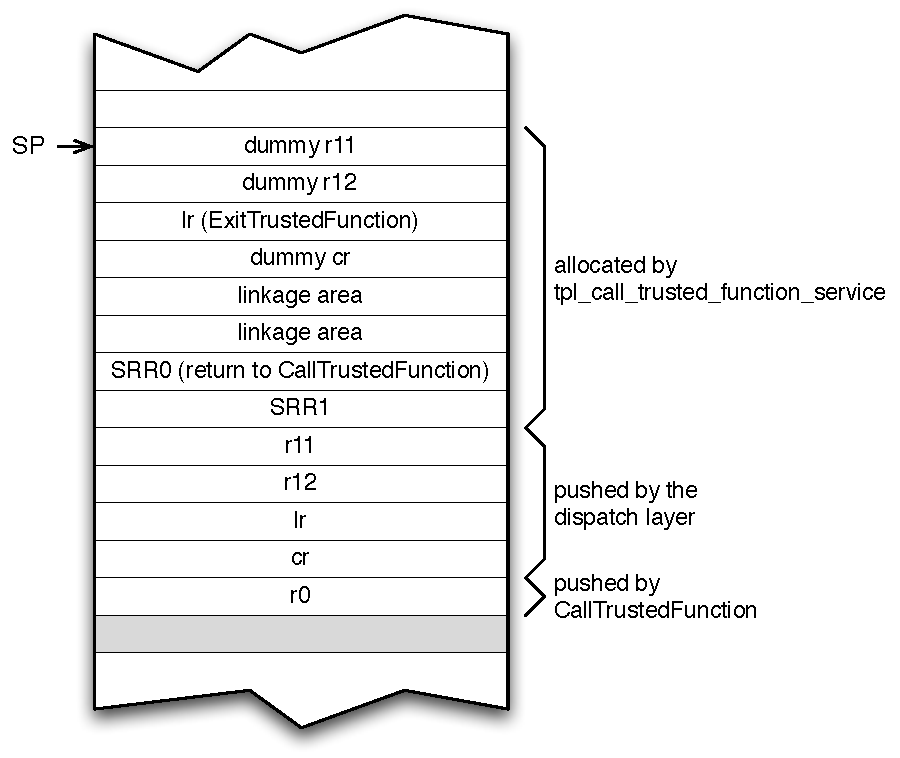
\includegraphics[scale=.6]{pictures/TFStack1} 
\end{minipage}
\begin{minipage}{0.35\textwidth}
  \caption{Process stack mapping at the end of \cfunction{tpl_call_trusted_function_service}. \reg{r0}, at the bottom of the stack has been pushed by \api{CallTrustedFunction}. \reg{cr} to \reg{r11} has been pushed by the dispatch layer. \reg{SRR0} and \reg{SRR1} are saved here by \cfunction{tpl_call_trusted_function_service} to be able to go back to the calling process. Above, the linkage area allows the trusted function to call functions. Above, a frame that will be used by the dispatch layer to restore an execution context for the trusted function is built.}\label{fig:tfstackmapping}
\end{minipage}
\end{figure}

\subsubsection{Setting the trusted function address}

The \reg{SRR0} saved by the dispatch layer after the \api{CallTrustedFunction} is changed to the address of the trusted function. This way, instead of returning to the caller, the trusted function will be executed.

\begin{lstlisting}
  lis   r11,TPL_HIG(tpl_trusted_fct_table)
  ori   r11,r11,TPL_LOW(tpl_trusted_fct_table)
  slwi  r0,r3,2
  lwzx  r12,r11,r0
  stw   r12,KS_SRR0(r1)
\end{lstlisting}

\subsubsection{Going back to the dispatch layer}

A simple \asfct{blr} goes back to the dispatch layer. The latter cleans up the process stack. Once the trusted function starts execution, the process stack is like that:

\begin{figure}[htbp] %  figure placement: here, top, bottom, or page
\begin{minipage}{0.5\textwidth}
    \centering
  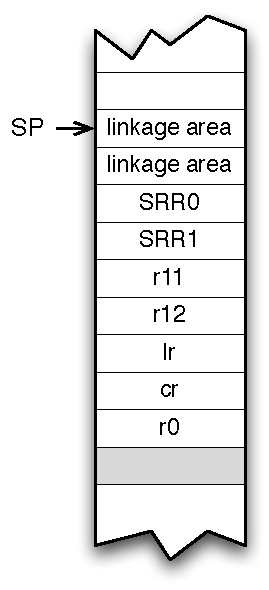
\includegraphics[scale=.6]{pictures/TFStack2} 
\end{minipage}
\begin{minipage}{0.5\textwidth}
  \caption{Process stack mapping when the trusted function starts its execution.}\label{fig:tfstackmapping2}
\end{minipage}
\end{figure}

\subsection{The ExitTrustedFunction service}\label{sec:exittfppc}

When a trusted function finishes, the context of the \api{CallTrustedFunction} must be restored to return to the caller. \api{ExitTrustedFunction} does not need to be called explicitly because its address has been set as the return address of the trusted function by \cfunction{tpl_call_trusted_function_service}. Calling \api{ExitTrustedFunction} explicitly may result in an undefined behavior or in the crash of the calling process but see below. The mapping of the process stack at start of \cfunction{tpl_exit_trusted_function_service} is shown in figure \ref{fig:ETFstack1}.

\begin{figure}[htbp] %  figure placement: here, top, bottom, or page
\begin{minipage}{0.4\textwidth}
    \centering
  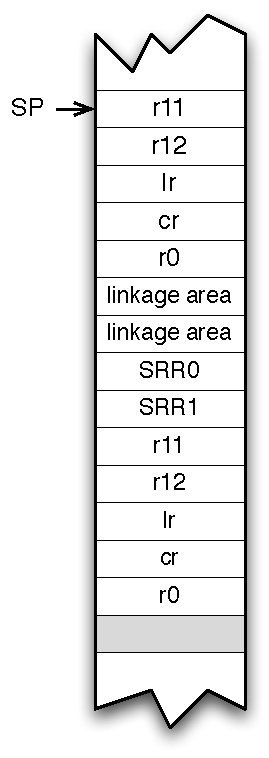
\includegraphics[scale=.6]{pictures/ETFStack1} 
\end{minipage}
\begin{minipage}{0.6\textwidth}
  \caption{Process stack mapping when the \cfunction{tpl_exit_trusted_function_service} function starts its execution.}\label{fig:ETFstack1}
\end{minipage}
\end{figure}

First, \cfunction{tpl_exit_trusted_function_service} decrements the trusted counter of the calling process. A particular attention must be given to this point because by building a fake stack frame and calling Explicitly \api{ExitTrustedFunction} to underflow this counter, a process could get a full access to the memory. So the counter is tested before to avoid to go under 0.

\begin{lstlisting}[language=C]
  lwz   r11,KS_KERN_PTR(r1) /* get the ptr to tpl_kern */
  lwz   r11,12(r11)         /* get the ptr to the runnning process desc */
  lwz   r12,4(r11)          /* get trusted_count member */
  /*
   * Warning, the trusted counter has to be check (compared to 0) to
   * avoid to decrement it if it is already 0. Without that a process
   * could build an had-hoc stack an call explicitly ExitTrustedFunction
   * to get access to all the memory.
   */
  cmpwi r12,0               /* check it is not already at 0 */
  beq   cracker_in_action   /* uh uh */
  subi  r12,r12,1           /* decrement it */
  stw   r12,4(r11)          /* put it back in the process desc */
\end{lstlisting}

\cfunction{tpl_exit_trusted_function_service} has to remove from the process stack the frame that was built by \cfunction{tpl_call_trusted_function_service}, restore \reg{SRR0} and \reg{SRR1} before returning to the dispatch layer.

\begin{lstlisting}[language=C]
cracker_in_action:
  
  /*
   * get the process stack pointer
   */
  lwz   r11,KS_SP(r1)
  
  /*
   * get back the SRR0 and SRR1
   */
  lwz   r12,PS_SRR0_OUT(r11)
  stw   r12,KS_SRR0(r1)
  lwz   r12,PS_SRR1_OUT(r11)
  stw   r12,KS_SRR1(r1)
  
  /*
   * free the process stack and update it in the kernel stack
   */
  addi  r11,r11,PS_TRUSTED_FOOTPRINT_OUT
  stw   r11,KS_SP(r1)
  
  /*
   * that's all
   */
  blr
\end{lstlisting}

\subsection{Execution of the OS Applications startup and shutdown hooks}

These hooks are executed from the kernel but with the access right of a task belonging to the OS Application. The \sysgen\ should choose one of the tasks of the OS Application to be used as context to execute the OS Application startup and shutdown hooks. Execution of an OS Application startup hook is done by the \cfunction{tpl_call_startup_hook_and_resume} function. The argument of this function is a function pointer to the hook. Similarly execution of an OS Application shutdown hook is done by the \cfunction{tpl_call_shutdown_hook_and_resume} function. These functions end by a call to \api{NextStartupHook} and \api{NextShutdownHook} services respectively to cycle through the hooks.

\subsection{The MPC5510 Memory Protection Unit}

The access control rights of the memory region descriptor rules the access of 5 bus masters (labeled from 4 to 0). Unused bus masters are set to the same access right for all the regions. Bus master 4 is used for factory testing only, so the access rights should be set to no access. Bus master 3 is the Flexray controller. Since it is not used in the current version of Trampoline, it is set to no access too. Bus master 2 is the DMA controller and for the same reason it is set to no access. Bus master 1 is the Z0 core. Again it is set to no access.

The access control rights register has the following bit usage:

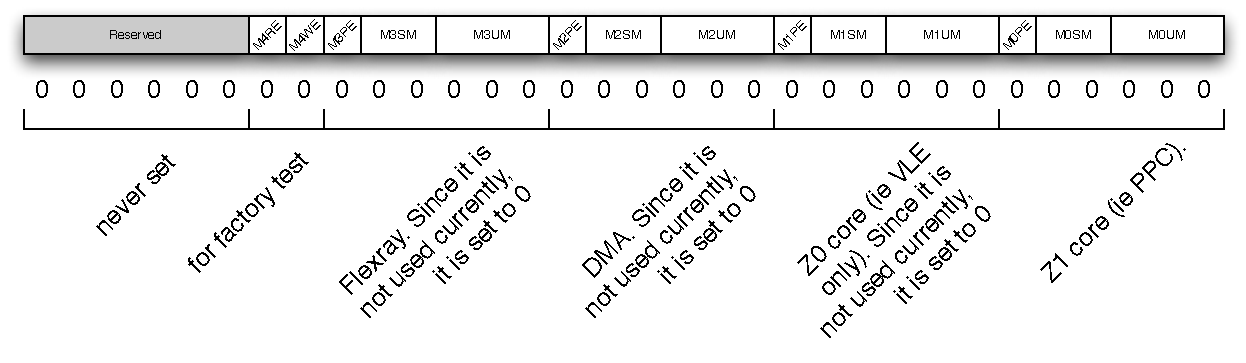
\includegraphics[width=\textwidth]{pictures/MPUacr.pdf} 

Bus master 4 is a special case. The 2 bits have the following meaning:

\rowcolors{1}{white}{light-gray}
\begin{longtable}[c]{l|p{5.15in}}
{\bf Bit}&{\bf Meaning}\\
\hline
\dreg{M4RE} & If set to 1, bus master 4 may {\bf read} memory in the region. If 0, no read is allowed\\
\dreg{M4WE} & If set to 1, bus master 4 may {\bf write} memory in the region. If 0, no write is allowed\
\end{longtable}

So in our case, these bits are set to 0.

Of course, other bus masters have more sophisticated access right:

\rowcolors{1}{white}{light-gray}
\begin{longtable}[c]{l|p{5.15in}}
{\bf Bit}&{\bf Meaning}\\
\hline
\dreg{MxPE} & The PID Enable bit. Set to 0 in our case\\
\dreg{MxSM} & These 2 bits rules the supervisor mode access control with the following meaning: $00=rwx$, $01=rx$, $10=rw$, $11=$ \textit{same as defined by \dreg{MxUM}}. In our case, it is set to $00$ for code and constants and to $11$ for data.\\
\dreg{MxUM} & These 2 bits rules the user mode access control. The first bit means $r$, the second one $w$ and the third one $x$.
\end{longtable}

Trampoline uses 4 descriptors:

\rowcolors{1}{white}{light-gray}
\begin{longtable}{l|p{1.9in}|p{2.6in}}
{\bf Descriptor} & {\bf Usage} & {\bf \dreg{MxUM} value}\\
\hline
\dreg{MPU_RGD0} & Constants and program\footnote{This region is set to the whole addressing space. This is not definitive and should be improved because reading a peripheral control register should be protected. So an additional descriptor has to be used to allow the kernel (supervisor mode) a complete access on all the memory space and no access at all for applications (user mode).}. & $rwx=00$ for supervisor mode, $rx=101$ for user mode.\\
\dreg{MPU_RGD1} & Private variables of the process. & $rw=110$ for supervisor and user mode.\\
\dreg{MPU_RGD2} & Stack of the process. & $rw=110$ for supervisor and user mode.\\
\dreg{MPU_RGD3} & Variables of the OS Application if OS Applications are used. & $rw=110$ for supervisor and user mode.\\
\end{longtable}

So values of access control bits should be:

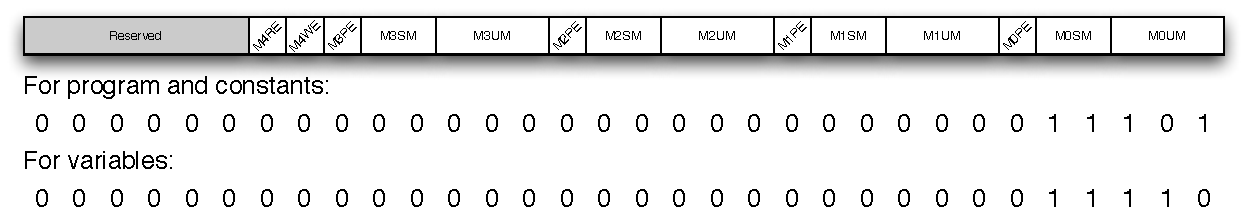
\includegraphics[width=\textwidth]{pictures/MPUprog.pdf} 

So in hexa:

\rowcolors{1}{white}{light-gray}
\begin{longtable}{l|l}
{\bf Kind} & {\bf Value}\\
\hline
Program region access & $0x00000005$\\
Variable region access & $0x0000001E$\\
\end{longtable}

\subsubsection{What happen in case of memory protection violation ?}

Two exception handler are used to handle a memory protection violation, one for data access, one for code access.

The Data Storage exception is tied to the IVOR~2 vector (VPR offset = 0x020), see page 8-2 of the {\em MPC5510 Microcontroller Family Reference Manual}.

The Instruction Storage exception is tied to the IVOR~3 vector (VPR offset = 0x030), see page 8-2 of the {\em MPC5510 Microcontroller Family Reference Manual}.

However, it appears one of these exceptions is raised when the processor is in user mode. The behavior is different in supervisor mode {\em to be completed}.

\section{ARM -- Common conventions}

\subsection{File hierarchy}

\subsection{Common definitions}

\subsection{Bootstraping}

The bootstrap must be made in specific ARM port and must call the \cfunction{main} function. If \cfunction{main} ever returns, the bootstrap code must fall into an infinite loop.

As a reason, many ARM architectures needs early specific and required initializations. This includes steps like memory mapping configuration, DRAM controller configuration, ...

Besides specific initializations, the bootstrap should :
\begin{itemize}
\item initialize stack pointer for every ARM exception modes
\item keep all external interrupts locked (will be unlocked at the first task context loading)
\item call \cfunction{main} in "system" mode (0x1F)
\end{itemize}

\subsection{Stacks}

\subsection{Interrupt management}

Kernel is not interruptible. So hardware interrupt source are disabled entering in kernel (via any case in system call, interrupt request, abort, ...).

But kernel shall be reentrant via system call (because kernel hooks can call some system calls).

\subsubsection{Interrupt and category classification}

All ARM IRQ are category 2 ISR.

All ARM FIQ are category 1 ISR.

\subsubsection{Vector table}

Each ARM exception vector points on a so called "primary" subprogram (like \cfunction{tpl\_primary\_syscall\_handler}).

To be located at address 0x00000000, this vector table is assigned to a specific section named \cfunction{.vectbl}. The linker script uses this section name to output it to address 0x00000000.

\subsubsection{System call}

\subsubsection{IRQ handling}

\subsubsection{FIQ handling}

\section{ARM -- Armadeus APF27 board}

\subsection{Debugging with Abatron BDI2000 or BDI3000 JTAG probe}

A configuration file is provided in \file{machines/arm/armadeus-apf27/bdi-config}.

To enable JTAG, if your APF27 has a FPGA, you must load the FPGA to wake it up (TO DO : explain how to do this...).

To start a debug session, follow these steps :
\begin{enumerate}
\item connects everything together
\item power up everything
\item reset the APF27 (S2 on APF27-Dev)
\item stop u-boot before it loads Linux (if MMU is started, you won't be able to load anything)
\item telnet your BDI
\item type \cfunction{reset} command in the BDI shell
\item start GDB session (\cfunction{target remote ...})
\end{enumerate}

\subsection{Configuration}

All configuration of port is done in \file{apf27\_config.h}.

\subsubsection{Stacks}

Stacks' size (stack of each exception mode) can be adjusted via the following constants. Remember that the size must be aligned to 4.

\subsubsection{CPU caches}

By default, CPU caches are disabled (for real time determinism).

\subsection{Memory mapping}

This port can be use in one of these three configurations :
\begin{enumerate}
\item No memory mapping (and thus no memory protection)
\item Memory mapping without memory protection
\item Memory mapping and memory protection
\end{enumerate}

\subsection{Memory protection}

To be written...

Some points to explain :
\begin{itemize}
\item FCSE mechanism is not used by this port (if someone is interested by this work, she's welcome)
\item address translation is not used, all VMA equals physical address
\end{itemize}

\subsubsection{MMU tables generation principle}

To be written...

Some points to explain :
\begin{itemize}
\item MMU is not disabled in privileged mode, but all useful memory areas are accessible. Thus, we hope we can find bugs easily in privіleged code.
\item useful memory areas, except processes and applications ones, are configured as accessible (read and write) in privileged mode. These memory areas are called system areas
\item some memory areas needs to be accessible by anyone (API, GCC builtin functions, common libraries, ...), they are called common areas (they are read only for unprivileged contexts)
\item there is one translation table for each process
\item all translation tables have the same system and common areas
\item there is one page table set for each process. Page tables are fine page tables. Table entries are tiny page descriptors.
\item the number of page table in a set depends on the size of the whole trampoline and application memory footprint. Then this information is given by linker via a symbol which is used by the MMU driver.
\item Page tables are accessed via a macro, as they are allocated by linker (and we cannot know the number of page tables)
\end{itemize}

\section{ARM -- Simtec EB675001 board}

\subsection{Memory map and hardware resources}

Talk about configured memory map (use of DRAM, where the bootstrap would be flashed, \ldots).

Tell which hardware resources are used by the kernel.

\subsection{Booting}

There is two way to start Trampoline on APF27 :
\begin{itemize}
\item from ELF image (in file usually called \file{trampoline})
\item from raw binary image (in file usually called \file{trampoline.bin})
\end{itemize}

\subsubsection{Booting from ELF image}

Load image with your ELF loader (the file is usually named \file{trampoline}). This can be GDB via a JTAG probe for example. Then, just start execution from \cfunction{tpl\_arm\_bootstrap\_entry} entry point. Here are commands you can type in GDB :
\begin{lstlisting}
(gdb) load
(gdb) set $pc=tpl_arm_bootstrap_entry
(gdb) break main
(gdb) continue
\end{lstlisting}

\subsubsection{Booting from raw binary image}

Load image with your binary loader to 0xA0000000 memory address. Then just start execution at this point (0xA0000000).

With u-boot, you can type these commands :
\begin{lstlisting}
BIOS> tftpboot 0xA0000000 192.168.5.20:trampoline.bin
BIOS> go 0xA0000000
\end{lstlisting}

\subsection{Internal kernel drivers}

\subsection{Hardware interrupts handling}

\subsection{Idle task}

\subsection{Exceptions handling}


\subsection{Kernel sleep service}



\part{The Goil system generator}
%!TEX root = ./trampoline.tex

\chapter{The Goil templates}

Goil includes a template interpreter which is used for file generation. Goil generates the structures needed by trampoline to compile the application and may generate other files like a memory mapping file \file{MemMap.h}, the compiler abstraction files, \file{Compiler.h} and \file{Compiler\_cfg.h} and a linker script depending on which attributes you set in the OIL file. 

A template is a file which is located in the default template directory (set with the environment variable \envvar{GOIL\_TEMPLATES} or with the \longprogramopt{templates} option on the command line) or in the directory of your project. Goil starts by looking for a template in the directory of your project, then, if the template is not found, in the default templates directory.

Four sets of templates are used:
\begin{itemize}
\item code generation templates that are located in the \file{code} subdirectory of the template directory;
\item build system templates that are located in the \file{build} subdirectory;
\item compiler dependent stuff in the \file{compiler} subdirectory and
\item linker script templates in the \file{linker} subdirectory.
\end{itemize}

Templates are written using a simple language which allow to access the application configuration data and to mix them with text to produce files.

Files are produced by a template program located in the \file{root.goilTemplate} file which is as the root of the template directory. By default the following files are produced:
\begin{itemize}
\item \file{tpl\_app\_config.c} by using the \file{tpl\_app\_config.c.goilTemplate} file
\item \file{tpl\_app\_config.h} by using the \file{tpl\_app\_config.h.goilTemplate} file
\item \file{Makefile} (if option \programopt{g} or \longprogramopt{generate-makefile} is given) by using the \file{Makefile.goilTemplate} file
\item \file{script.ld} (if memory mapping is used and if the default name is not changed) by using the \file{script.goilTemplate} file
\item \file{MemMap.h} (if memory mapping is used) by using the \file{MemMap.h.goilTemplate} file
\item \file{Compiler.h} (if memory mapping is used) by using the \file{Compiler.h.goilTemplate} file
\item \file{Compiler\_Cfg.h} (if memory mapping is used) by using the\\\file{Compiler\_Cfg.h.goilTemplate} file
\end{itemize}

\section{The configuration data}

The configuration data are computed by Goil from the OIL source files, from the options on the command line and from the \file{target.cfg} file. They are available as a set of predefined boolean, string, integer or list variables. All these variables are in capital letters.

\warning{Some configuration data are not listed here because they are dependent on the target. For instance, the \member{STACKSIZE} data may be an attribute of each item of a \var{TASKS} list for ppc target but are missing for the c166 target.}

\subsection{The \var{PROCESSES}, \var{TASKS}, \var{BASICTASKS}, \var{EXTENDEDTASKS}, \var{ISRS1} and \var{ISRS2} lists}

Theses variables are lists where informations about the processes\footnote{In Trampoline, a process is a task or an ISR category 2.} used in the application are stores:

\rowcolors{1}{white}{light-gray}
\begin{longtableii}{p{1.2in}|p{4in}}{var}{List}{Content}
  \lineii{PROCESSES}
  {the list of processes. The items are sorted in the following order: extended tasks, then basic tasks, then ISRs category 2.}
  \lineii{TASKS}
  {the list of tasks, basic and extended. The items are sorted in the following order: extended tasks, then basic tasks.}
  \lineii{BASICTASKS}
  {the list of basic tasks.}
  \lineii{EXTENDEDTASKS}
  {the list of extended tasks.}
  \lineii{ISRS1}
  {the list of ISR category 1.}
  \lineii{ISRS2}
  {the list of ISR category 2.}
\end{longtableii}

Each item of these lists has the following attributes:

\rowcolors{1}{white}{light-gray}
\begin{longtableiii}{p{1.6in}|l|p{3in}}{member}{Item}{Type}{Content}
  \lineiii{NAME}
  {string}
  {the name of the process.}
  \lineiii{PROCESSKIND}
  {string}
  {the kind of process: \stringlit{Task} or \stringlit{ISR}.}
  \lineiii{EXTENDEDTASK}
  {boolean}
  {true if the process is an extended task, false otherwise.}
  \lineiii{NONPREEMPTABLE}
  {boolean}
  {true if the process is a non-preemptable task, false otherwise.}
  \lineiii{PRIORITY}
  {integer}
  {the priority of the process.}
  \lineiii{ACTIVATION}
  {integer}
  {the number of activation of a task. 1 for and extended task or an ISR.}
  \lineiii{AUTOSTART}
  {boolean}
  {true if the process is an autostart task, false otherwise.}
  \lineiii{USEINTERNALRESOURCE}
  {boolean}
  {true if the process is a task that uses an internal resource, false otherwise.}
  \lineiii{INTERNALRESOURCE}
  {string}
  {the name of the internal resource if the process is a task that uses an internal resource, empty string otherwise.}
  \lineiii{RESOURCES}
  {list}
  {The resources used by the process. Each item has the following attribute: \member{NAME}}
\end{longtableiii}

\subsection{The \var{COUNTERS}, \var{HARDWARECOUNTERS} and \var{SOFTWARECOUNTERS} lists}

This list contains all the informations about the counters used in the application, including the \var{SystemCounter}.

\rowcolors{1}{white}{light-gray}
\begin{longtableii}{p{1.5in}|p{3.7in}}{var}{List}{Content}
  \lineii{COUNTERS}
  {the list of counters, both hardware and software as long as the \var{SystemCounter}}
  \lineii{HARDWARECOUNTERS}
  {the list of hardware counters including the \var{SystemCounter}.}
  \lineii{SOFTWARECOUNTERS}
  {the list of software counters.}
\end{longtableii}

Each item of this list has the following attributes:

\rowcolors{1}{white}{light-gray}
\begin{longtableiii}{p{1.6in}|l|p{3in}}{member}{Item}{Type}{Content}
  \lineiii{NAME}
  {string}
  {the name of the counter.}
  \lineiii{TYPE}
  {string}
  {the type of counter: {\small\stringlit{HARDWARE_COUNTER}} or {\small\stringlit{SOFTWARE_COUNTER}}.}
  \lineiii{MAXALLOWEDVALUE}
  {integer}
  {the maximum allowed value of the counter.}
  \lineiii{MINCYCLE}
  {integer}
  {the minimum cycle value of the counter.}
  \lineiii{TICKPERBASE}
  {integer}
  {the number of ticks needed to increment the counter.}
  \lineiii{SOURCE}
  {string}
  {the interrupt source name of the counter. This can be used to wrap interrupt vector to a counter incrementation function}
\end{longtableiii}

\subsection{The \var{EVENTS} list}

This list contains the informations about the events of the application. Each item has the following attributes:

\rowcolors{1}{white}{light-gray}
\begin{longtableiii}{p{1.6in}|l|p{3in}}{member}{Item}{Type}{Content}
  \lineiii{NAME}
  {string}
  {the name of the event.}
  \lineiii{MASK}
  {integer}
  {the mask of the event.}
\end{longtableiii}

\subsection{The \var{ALARMS} list}

This list contains the informations about the alarms of the application. Each item has the following attributes:

\rowcolors{1}{white}{light-gray}
\begin{longtableiii}{p{1.6in}|l|p{3in}}{member}{Item}{Type}{Content}
  \lineiii{NAME}
  {string}
  {the name of the alarm.}
  \lineiii{COUNTER}
  {string}
  {the name of the counter that drives the alarm.}
  \lineiii{ACTION}
  {string}
  {the action to be done when the alarm expire. It can take the following values: \stringlit{setEvent}, \stringlit{activateTask} and \stringlit{callback}. The last action is not available in Autosar mode.}
  \lineiii{TASK}
  {string}
  {the name of the task on which the action is performed. This attribute is defined for \stringlit{setEvent} and \stringlit{activateTask} actions only.}
  \lineiii{EVENT}
  {string}
  {the name of the event to set on the target task. This attribute is defined for \stringlit{setEvent} action only.}
  \lineiii{AUTOSTART}
  {boolean}
  {true if the alarm is autostart, false otherwise}
  \lineiii{ALARMTIME}
  {integer}
  {the alarm time of the alarm. This attribute is set if \member{AUTOSTART} is true}
  \lineiii{CYCLETIME}
  {integer}
  {the cycle time of the alarm. This attribute is set if \member{AUTOSTART} is true}
  \lineiii{APPMODE}
  {string}
  {the application mode in which the alarm is autostart. This attribute is set if \member{AUTOSTART} is true}
\end{longtableiii}

\subsection{The \var{REGULARRESOURCES} and \var{INTERNALRESOURCES} lists}

These lists contains the informations about the resources of the application.

\rowcolors{1}{white}{light-gray}
\begin{longtableii}{p{1.5in}|p{3.7in}}{var}{List}{Content}
  \lineii{REGULARRESOURCES}
  {the list of STANDARD and LINKED resources.}
  \lineii{INTERNALRESOURCES}
  {the list of INTERNAL resources.}
\end{longtableii}

Each item has the following attributes:

\rowcolors{1}{white}{light-gray}
\begin{longtableiii}{p{1.6in}|l|p{3in}}{member}{Item}{Type}{Content}
  \lineiii{NAME}
  {string}
  {the name of the resource.}
  \lineiii{PRIORITY}
  {integer}
  {the priority of the resource.}
  \lineiii{TASKUSAGE}
  {list}
  {the list of tasks that use the resource. Each item of this list has an attribute \member{NAME} which is the name of the task.}
  \lineiii{ISRUSAGE}
  {list}
  {the list of ISRs that use the resource. Each item of this list has an attribute \member{NAME} which is the name of the ISR.}
\end{longtableiii}

\subsection{The \var{MESSAGES}, \var{SENDMESSAGES} and \var{RECEIVEMESSAGES} lists}

These lists contain the informations about the messages of the application.

\rowcolors{1}{white}{light-gray}
\begin{longtableii}{p{1.5in}|p{3.7in}}{var}{List}{Content}
  \lineii{MESSAGES}
  {the list of messages, both send and receive message.}
  \lineii{SENDMESSAGES}
  {the list of send messages.}
  \lineii{RECEIVEMESSAGES}
  {the list of receive messages.}
\end{longtableii}

Each item has the following attributes

\rowcolors{1}{white}{light-gray}
\begin{longtableiii}{p{1.6in}|l|p{3in}}{member}{Item}{Type}{Content}
  \lineiii{NAME}
  {string}
  {the name of the message.}
  \lineiii{MESSAGEPROPERTY}
  {string}
  {the type of the message. It can be {\small\stringlit{RECEIVE\_ZERO\_INTERNAL}, \stringlit{RECEIVE\_UNQUEUED\_INTERNAL}, \stringlit{RECEIVE\_QUEUED\_INTERNAL}, \stringlit{SEND\_STATIC\_INTERNAL}, \stringlit{SEND\_ZERO\_INTERNAL} or \stringlit{RECEIVE\_ZERO\_SENDERS}}.}
  \lineiii{NEXT}
  {string}
  {the name of the next message in a receive message chain. This attribute is defined for receive messages only.}
  \lineiii{SOURCE}
  {string}
  {the name of the send message which is connected to the receive message. This attribute is defined for receive messages only.}
  \lineiii{CTYPE}
  {string}
  {the C language type of the message. This attribute is not defined for {\small\stringlit{RECEIVE\_ZERO\_INTERNAL}} and  {\small\stringlit{SEND\_ZERO\_INTERNAL}} messages.}
  \lineiii{INITIALVALUE}
  {string}
  {initial value of the receive message. This attribute is defined for {\small\stringlit{RECEIVE\_UNQUEUED\_INTERNAL}} and  {\small\stringlit{RECEIVE\_ZERO\_SENDERS}} messages only.}
  \lineiii{QUEUESIZE}
  {integer}
  {queue size of a receive queued message. This attribute is defined for {\small\stringlit{RECEIVE\_QUEUED\_INTERNAL}} messages only.}
  \lineiii{TARGET}
  {string}
  {target message of a send message. This is the first message in a receive message chain. This attribute is defined for {\small\stringlit{SEND\_STATIC\_INTERNAL}} and {\small\stringlit{SEND\_ZERO\_INTERNAL}} messages only.}
  \lineiii{FILTER}
  {string}
  {the kind of filter to apply. This attribute may take the following values: {\small\stringlit{ALWAYS}, \stringlit{NEVER}, \stringlit{MASKEDNEWEQUALSX}, \stringlit{MASKEDNEWDIFFERSX}, \stringlit{NEWISEQUAL}, \stringlit{NEWISDIFFERENT}, \stringlit{MASKEDNEWEQUALSMASKEDOLD}, \stringlit{MASKEDNEWDIFFERSMASKEDOLD}, \stringlit{NEWISWITHIN}, \stringlit{NEWISOUTSIDE}, \stringlit{NEWISGREATER}, \stringlit{NEWISLESSOREQUAL}, \stringlit{NEWISLESS}, \stringlit{NEWISGREATEROREQUAL}} or {\small\stringlit{ONEEVERYN}}.}
  \lineiii{MASK}
  {integer}
  {Mask of the filter when needed. This attribute is defined for {\small\stringlit{MASKEDNEWEQUALSX}, \stringlit{MASKEDNEWDIFFERSX}, \stringlit{MASKEDNEWEQUALSMASKEDOLD}} and {\small\stringlit{MASKEDNEWDIFFERSMASKEDOLD}} filters only.}
  \lineiii{X}
  {integer}
  {Value of the filter when needed. This attribute is defined for {\small\stringlit{MASKEDNEWEQUALSMASKEDOLD}} and {\small\stringlit{MASKEDNEWDIFFERSX}} filters only.}
  \lineiii{MIN}
  {integer}
  {Minimum value of the filter when needed. This attribute is defined for {\small\stringlit{NEWISWITHIN}} and {\small\stringlit{NEWISOUTSIDE}} filters only.}
  \lineiii{MAX}
  {integer}
  {Maximum value of the filter when needed. This attribute is defined for {\small\stringlit{NEWISWITHIN}} and {\small\stringlit{NEWISOUTSIDE}}}     
  \lineiii{PERIOD}
  {integer}
  {Period of the filter. This attribute is defined for {\small\stringlit{ONEEVERYN}} filter only.}
  \lineiii{OFFSET}
  {integer}
  {Offset of the filter. This attribute is defined for {\small\stringlit{ONEEVERYN}} filter only.}
  \lineiii{ACTION}
  {string}
  {the action (or notification) to be done when the message is delivered. It can take the following values: \stringlit{setEvent} or \stringlit{activateTask}.}
  \lineiii{TASK}
  {string}
  {the name of the task on which the notification is performed. This attribute is defined for \stringlit{setEvent} and \stringlit{activateTask} actions only.}
  \lineiii{EVENT}
  {string}
  {the name of the event to set on the target task. This attribute is defined for \stringlit{setEvent} notification only.}
\end{longtableiii}

\subsection{The \var{SCHEDULETABLES} list}

This list contains the informations about the schedule tables of the application.

\rowcolors{1}{white}{light-gray}
\begin{longtableiii}{p{1.6in}|l|p{3in}}{member}{Item}{Type}{Content}
  \lineiii{NAME}
  {string}
  {the name of the schedule table.}
  \lineiii{COUNTER}
  {string}
  {the name of the counter which drives the schedule table.}
  \lineiii{PERIODIC}
  {boolean}
  {true if the schedule table is a periodic one, false otherwise.}
  \lineiii{SYNCSTRATEGY}
  {string}
  {the synchronization strategy of the schedule table. This attribute may take the following values: {\small\stringlit{SCHEDTABLE_NO_SYNC}, \stringlit{SCHEDTABLE_IMPLICIT_SYNC}} or {\small\stringlit{SCHEDTABLE_EXPLICIT_SYNC}}.}
  \lineiii{PRECISION}
  {integer}
  {the precision of the synchronization. This attribute is define when \member{SYNCSTRATEGY} is {\small\stringlit{SCHEDTABLE_EXPLICIT_SYNC}}.}
  \lineiii{STATE}
  {string}
  {the state of the schedule table. This attribute may take the following values: {\small\stringlit{SCHEDULETABLE_STOPPED}, \stringlit{SCHEDULETABLE_AUTOSTART_SYNCHRON}, \stringlit{SCHEDULETABLE_AUTOSTART_RELATIVE}} or {\small\stringlit{SCHEDULETABLE_AUTOSTART_ABSOLUTE}}.}
  \lineiii{DATE}
  {integer}
  {the start date of the schedule table. This attribute has an actuel value when \member{STATE} is {\small\stringlit{SCHEDULETABLE_AUTOSTART_RELATIVE}} or {\small\stringlit{SCHEDULETABLE_AUTOSTART_ABSOLUTE}}, otherwise it is set to 0.}
  \lineiii{LENGTH}
  {integer}
  {The length of the schedule table.}
  \lineiii{EXPIRYPOINTS}
  {list}
  {The expiry points of the schedule table. See the following table for items attributes.}
\end{longtableiii}

Each item of the \member{EXPIRYPOINTS} list has the following attributes:

\rowcolors{1}{white}{light-gray}
\begin{longtableiii}{p{1.6in}|l|p{3in}}{member}{Item}{Type}{Content}
  \lineiii{ABSOLUTEOFFSET}
  {integer}
  {the absolute offset of the expiry points.}
  \lineiii{RELATIVEOFFSET}
  {integer}
  {the relative offset of the expiry points from the previous expiry point.}
  \lineiii{MAXRETARD}
  {integer}
  {maximum retard to keep the schedule table synchronous.}
  \lineiii{MAXADVANCE}
  {integer}
  {maximum advance to keep the schedule table synchronous.}
  \lineiii{ACTIONS}
  {list}
  {the actions to perform on the expiry point. See the following table for items attributes.}
\end{longtableiii}

Each item of the \member{ACTIONS} list has the following attributes:

\rowcolors{1}{white}{light-gray}
\begin{longtableiii}{p{1.6in}|l|p{3in}}{member}{Item}{Type}{Content}
  \lineiii{ACTION}
  {string}
  {the action to be done when the alarm expire. It can take the following values: \stringlit{setEvent}, \stringlit{activateTask}, \stringlit{incrementCounter} and \stringlit{finalizeScheduleTable}.}
  \lineiii{TASK}
  {string}
  {the name of the task on which the action is performed. This attribute is defined for \stringlit{setEvent} and \stringlit{activateTask} actions only.}
  \lineiii{EVENT}
  {string}
  {the name of the event to set on the target task. This attribute is defined for \stringlit{setEvent} action only.}
  \lineiii{TARGETCOUNTER}
  {string}
  {the name of the counter to increment. This attribute is defined for \stringlit{incrementCounter} action only.}
\end{longtableiii}

\subsection{The \var{OSAPPLICATIONS} list}

This list contains the informations about the OS Applications of the application.

\rowcolors{1}{white}{light-gray}
\begin{longtableiii}{p{2.1in}|l|p{2.5in}}{member}{Item}{Type}{Content}
  \lineiii{NAME}
  {string}
  {the name of the OS Application.}
  \lineiii{RESTART}
  {string}
  {the name of the restart task. This attribute is not defined is there is no restart task for the OS Application.}
  \lineiii{PROCESSACCESSVECTOR}
  {string}
  {access right for the processes}
  \lineiii{PROCESSACCESSITEMS}
  {string}
  {access right for the processes as bytes in a table}
  \lineiii{PROCESSACCESSNUM}
  {integer}
  {number of elements in the previous table}
  \lineiii{ALARMACCESSVECTOR}
  {string}
  {access right for the alarms}
  \lineiii{ALARMACCESSITEMS}
  {string}
  {access right for the alarms as bytes in a table}
  \lineiii{ALARMACCESSNUM}
  {integer}
  {number of elements in the previous table}
  \lineiii{RESOURCEACCESSVECTOR}
  {string}
  {access right for the resources}
  \lineiii{RESOURCEACCESSITEMS}
  {string}
  {access right for the resources as bytes in a table}
  \lineiii{RESOURCEACCESSNUM}
  {integer}
  {number of elements in the previous table}
  \lineiii{SCHEDULETABLEACCESSVECTOR}
  {string}
  {access right for the schedule tables}
  \lineiii{SCHEDULETABLEACCESSITEMS}
  {string}
  {access right for the schedule tables as bytes in a table}
  \lineiii{SCHEDULETABLEACCESSNUM}
  {integer}
  {number of elements in the previous table}
  \lineiii{COUNTERACCESSVECTOR}
  {string}
  {access right for the software counters}
  \lineiii{COUNTERACCESSITEMS}
  {string}
  {access right for the software counters as bytes in a table}
  \lineiii{COUNTERACCESSNUM}
  {integer}
  {number of elements in the previous table}
  \lineiii{PROCESSES}
  {list}
  {list of the processes that belong to the OS Application. Each item has an attribute \member{NAME} which is the name of the process.}
  \lineiii{HASSTARTUPHOOK}
  {boolean}
  {true if the OS Application has a startup hook.}
  \lineiii{HASSHUTDOWNHOOK}
  {boolean}
  {true if the OS Application has a shutdown hook.}
  \lineiii{TASKS}
  {list}
  {list of the tasks that belong to the OS Application. Each item has an attribute \member{NAME} which is the name of the task.}
  \lineiii{ISRS}
  {list}
  {list of the ISRs that belong to the OS Application. Each item has an attribute \member{NAME} which is the name of the ISR.}
  \lineiii{ALARMS}
  {list}
  {list of the alarms that belong to the OS Application. Each item has an attribute \member{NAME} which is the name of the alarm.}
  \lineiii{RESOURCES}
  {list}
  {list of the resources that belong to the OS Application. Each item has an attribute \member{NAME} which is the name of the resource.}
  \lineiii{REGULARRESOURCES}
  {list}
  {list of the standard or linked resources that belong to the OS Application. Each item has an attribute \member{NAME} which is the name of the resource.}
  \lineiii{INTERNALRESOURCES}
  {list}
  {list of the internal resources that belong to the OS Application. Each item has an attribute \member{NAME} which is the name of the resource.}
  \lineiii{SCHEDULETABLES}
  {list}
  {list of the schedule tables that belong to the OS Application. Each item has an attribute \member{NAME} which is the name of the schedule table.}
  \lineiii{COUNTERS}
  {list}
  {list of the counters that belong to the OS Application. Each item has an attribute \member{NAME} which is the name of the counter.}
  \lineiii{MESSAGES}
  {list}
  {list of the messages that belong to the OS Application. Each item has an attribute \member{NAME} which is the name of the messages.}
\end{longtableiii}

\subsection{The \var{TRUSTEDFUNCTIONS} list}

This list contains the informations about the trusted functions of the application. Each item contains one attribute only.

\rowcolors{1}{white}{light-gray}
\begin{longtableiii}{p{1.6in}|l|p{3in}}{member}{Item}{Type}{Content}
  \lineiii{NAME}
  {string}
  {the name of the trusted function.}
\end{longtableiii}

\subsection{The \var{READLIST} list}

This list contains the informations about the ready list. Items are sorted by priority from 0 to the maximum computed priority. The only attribute of each item is the size of the queue.

\rowcolors{1}{white}{light-gray}
\begin{longtableiii}{p{1.6in}|l|p{3in}}{member}{Item}{Type}{Content}
  \lineiii{SIZE}
  {integer}
  {the size of the queue for the corresponding priority.}
\end{longtableiii}

\subsection{The \var{SOURCEFILES}, \var{CFLAGS}, \var{CPPFLAGS}, \var{ASFLAGS}, \var{LDFLAGS} and \var{TRAMPOLINESOURCEFILES} lists}

The \var{SOURCEFILES} list contains the source files as found in attributes \member{APP\_SRC} of the OS object in the OIL file.

\rowcolors{1}{white}{light-gray}
\begin{longtableiii}{p{1.6in}|l|p{3in}}{member}{Item}{Type}{Content}
  \lineiii{FILE}
  {string}
  {the source file name.}
\end{longtableiii}

The \var{CFLAGS} list contains the flags for the C compiler as found in attributes \member{CFLAGS} of the OS object in the OIL file.

\rowcolors{1}{white}{light-gray}
\begin{longtableiii}{p{1.6in}|l|p{3in}}{member}{Item}{Type}{Content}
  \lineiii{CFLAG}
  {string}
  {the C compiler flag.}
\end{longtableiii}

The \var{CPPFLAGS} list contains the flags for the C++ compiler as found in attributes \member{CPPFLAGS} of the OS object in the OIL file.

\rowcolors{1}{white}{light-gray}
\begin{longtableiii}{p{1.6in}|l|p{3in}}{member}{Item}{Type}{Content}
  \lineiii{CPPFLAG}
  {string}
  {the C++ compiler flag.}
\end{longtableiii}

The \var{ASFLAGS} list contains the flags for the assembler as found in attributes \member{ASFLAGS} of the OS object in the OIL file.

\rowcolors{1}{white}{light-gray}
\begin{longtableiii}{p{1.6in}|l|p{3in}}{member}{Item}{Type}{Content}
  \lineiii{ASFLAG}
  {string}
  {the assembler flag.}
\end{longtableiii}

The \var{LDFLAGS} list contains the flags for the linker as found in attributes \member{LDFLAGS} of the OS object in the OIL file.

\rowcolors{1}{white}{light-gray}
\begin{longtableiii}{p{1.6in}|l|p{3in}}{member}{Item}{Type}{Content}
  \lineiii{LDFLAG}
  {string}
  {the linker flag.}
\end{longtableiii}

The \var{TRAMPOLINESOURCEFILES} list contains the trampoline source files used by the application.

\rowcolors{1}{white}{light-gray}
\begin{longtableiii}{p{1.6in}|l|p{3in}}{member}{Item}{Type}{Content}
  \lineiii{DIRECTORY}
  {string}
  {the directory of the source file relative to the Trampoline root directory (\file{os}, \file{com} or \file{autosar}).}
  \lineiii{FILE}
  {string}
  {the source file name.}
\end{longtableiii}


\subsection{The \var{INTERRUPTSOURCES} list}

This list is extracted from the \file{target.cfg} file. Each item has the following attribute:

\rowcolors{1}{white}{light-gray}
\begin{longtableiii}{p{1.6in}|l|p{3in}}{member}{Item}{Type}{Content}
  \lineiii{NAME}
  {string}
  {the name of the interrupt source. This is one of the name used in the OIL file as value for the \member{SOURCE} attribute}
  \lineiii{NUMBER}
  {string}
  {the id of the interrupt source.}
\end{longtableiii}



\subsection{Scalar data}

The following scalar data are defined:

\rowcolors{1}{white}{light-gray}
\begin{longtableiii}{p{1.6in}|l|p{3in}}{member}{Data}{Type}{Content}
\lineiii{APPNAME}
{string}
{name of executable as given in the \member{APP\_NAME} attribute in the OS object} 
\lineiii{ARCH}
{string}
{name of the architecture. This is the first item in the target.} 
\lineiii{ASSEMBLEREXE}
{string}
{name of the assembler executable used. This is the \member{ASSEMBLER} attribute in the OS object. It is set to {\em as} by default. It is used for build dependent templates.} 
\lineiii{ASSEMBLER}
{string}
{name of the assembler used. This is the \member{ASSEMBLER} attribute in the \member{MEMMAP} attribute of the OS object. It is used for assembler dependent templates.} 
\lineiii{AUTOSAR}
{boolean}
{true if Trampoline is compiled with the Autosar extension.} 
\lineiii{BOARD}
{string}
{name of the board. This is the third item (if any) in the target.} 
\lineiii{CHIP}
{string}
{name of the chip. This is the second item (if any) in the target.} 
\lineiii{COMPILEREXE}
{string}
{name of the compiler executable used. This is the \member{COMPILER} attribute in the OS object. It is set to {\em gcc} by default. It is used for build dependent templates. Do not confuse with the \member{COMPILER} data.} 
\lineiii{COMPILER}
{string}
{name of the compiler used. This is the \member{COMPILER} attribute in the \member{MEMMAP} attribute of the OS object. It is used for compiler dependent templates.} 
\lineiii{CPUNAME}
{string}
{name given to the OIL CPU object} 
\lineiii{EXTENDED}
{boolean}
{true if Trampoline is compiled in extended error handling mode.} 
\lineiii{FILENAME}
{string}
{the name of the file which will be written as the result of the computation of the current template.} 
\lineiii{FILEPATH}
{string}
{the full absolute path of the file which will be written as the result of the computation of the current template.} 
\lineiii{NATIVEFILEPATH}
{string}
{the full absolute path of the file which will be written as the result of the computation of the current template in native OS format.} 
\lineiii{ITSOURCESLENGTH}
{integer}
{number of interrupt sources as defined in the \file{target.cfg} file.} 
\lineiii{LINKEREXE}
{string}
{name of the linker executable used. This is the \member{LINKER} attribute in the OS object. It is set to {\em gcc} by default. It is used for build dependent templates. Do not confuse with the \member{LINKER} data.} 
\lineiii{LINKER}
{string}
{name of the linker used. This is the \member{LINKER} attribute in the \member{MEMMAP} attribute of the OS object. It is used for linker dependent templates.} 
\lineiii{LINKSCRIPT}
{string}
{name of the link script file as given in the \member{MEMMAP} attribute of the OS object.} 
\lineiii{MAXTASKPRIORITY}
{integer}
{the highest computed priority among the tasks.} 
\lineiii{OILFILENAME}
{string}
{name of the root OIL source file} 
\lineiii{PROJECT}
{string}
{name of the project. The name of the project is the \programopt{p} (or \longprogramopt{project}) value if it is set or the name of the oil file without the extension.} 
\lineiii{SCALABILITYCLASS}
{integer}
{the Autosar scalability class used by the application. If Autosar is not enabled, \member{SCALABILITYCLASS} is set to 0.} 
\lineiii{TARGET}
{string}
{name of the target. This is the \programopt{t} (or \longprogramopt{target}) option value of goil.} 
\lineiii{TEMPLATEPATH}
{string}
{path to the template root directory. This is the \longprogramopt{templates} option value of goil or the value of the \envvar{GOIL\_TEMPLATES} environment variable.} 
\lineiii{TIMESTAMP}
{string}
{current date} 
\lineiii{TRAMPOLINEPATH}
{string}
{path to the trampoline root directory. This is the \member{TRAMPOLINE\_BASE\_PATH} attribute of the OS object. It defaults to ``..".} 
\lineiii{USECOMPILERSETTINGS}
{boolean}
{true if memory mapping is enabled (Goil generates the \file{Compiler.h} and \file{Compiler_Cfg.h} files and Trampoline includes them).} 
\lineiii{USEBUILDFILE}
{boolean}
{true if a build file is used for the project ie option \programopt{g} or \longprogramopt{generate-makefile} is given.} 
\lineiii{USECOM}
{boolean}
{true if the application uses OSEK COM.} 
\lineiii{USEERRORHOOK}
{boolean}
{true if Trampoline uses the Error Hook.} 
\lineiii{USEGETSERVICEID}
{boolean}
{true if Trampoline uses the service ids access macros.} 
\lineiii{USEINTERRUPTTABLE}
{boolean}
{true if the wrapping of interrupt vector to glue functions used to increment a counter or to activate an ISR2 (for instance) should be generated. The actual code generation is up to the port.} 
\lineiii{USELOGFILE}
{boolean}
{true if goil generates a log file, ie option \programopt{l} or \longprogramopt{logfile} is given.}
\lineiii{USEMEMORYMAPPING}
{boolean}
{true if memory mapping is enabled (Goil generates the \file{MemMap.h} file and Trampoline includes it).} 
\lineiii{USEMEMORYPROTECTION}
{boolean}
{true if Trampoline uses the Memory Protection.} 
\lineiii{USEOSAPPLICATION}
{boolean}
{true if Trampoline uses OS Applications.} 
\lineiii{USEPARAMETERACCESS}
{boolean}
{true if Trampoline uses the parmaters access macros.} 
\lineiii{USEPOSTTASKHOOK}
{boolean}
{true if Trampoline uses the Post-Task Hook.} 
\lineiii{USEPRETASKHOOK}
{boolean}
{true if Trampoline uses the Pre-Task Hook.} 
\lineiii{USEPROTECTIONHOOK}
{boolean}
{true if Trampoline uses the Protection Hook.} 
\lineiii{USERESSCHEDULER}
{boolean}
{true if Trampoline uses the RES_SCHEDULER resource.} 
\lineiii{USESHUTDOWNHOOK}
{boolean}
{true if Trampoline uses the Shutdown Hook.} 
\lineiii{USESTACKMONITORING}
{boolean}
{true if Trampoline uses the Stack Monitoring.} 
\lineiii{USESTARTUPHOOK}
{boolean}
{true if Trampoline uses the Startup Hook.} 
\lineiii{USESYSTEMCALL}
{boolean}
{true if services are called using a System Call (i.e. a software interrupt).} 
\lineiii{USETIMINGPROTECTION}
{boolean}
{true if Trampoline uses Timing Protection.} 
\lineiii{USETRACE}
{boolean}
{true if tracing is enabled.} 

\end{longtableiii}

\section{The Goil template language (or GTL)}

A template is a text file with file extension \file{.goilTemplate}. This kind of file mixes literal text with an embedded program. Some instructions (see section \ref{outputInstruction}) in the embedded program outputs text as a result of the program execution and this text is put in place of the instructions. The resulting file is then stored.

The template interpreter starts in literal text mode. Switching from literal text mode to program mode and back to text mode is done when a \character{\%} is encountered. A literal \character{\%} and a literal \character{\textbackslash} may be used by escaping them with a \character{\textbackslash}.

\section{GTL types}

GTL supports 5 types: \strong{string}, \strong{integer}, \strong{boolean}, \strong{list} and \strong{struct}. The 4 first types have readers %\footnote{All the readers available in the corresponding Galgas types are available}
to get informations about a variable. A reader is invoke with the following syntax:

\begin{lstlisting}
[expression reader]
\end{lstlisting}

A struct is an aggregate of data. The `::' allows to get a member of the struct. For instance one of the member of \var{TIMINGPROTECTION} is \member{TIMEFRAME} so to get \member{TIMEFRAME}, the following syntax is used:

\begin{lstlisting}
TIMINGPROTECTION::TIMEFRAME
\end{lstlisting}

\subsection{string readers}

The following readers are available for string variables:

\rowcolors{1}{white}{light-gray}
\begin{longtableiii}{p{2.2in}|l|p{2.4in}}{strong}{Item}{Type}{Meaning}
  \lineiii{HTMLRepresentation}
  {string}
  {this reader returns a representation of the string suitable for an HTML encoded representation. \character{\&} is encoded by \&amp; , \character{"} by \&quot; , \character{<} by \&lt; and \character{>} by \&gt; .}
  \lineiii{identifierRepresentation}
  {string}
  {this reader returns an unique representation of the string conforming to a C identifier. Any Unicode character that is not a latin letter is transformed into its hexadecimal code point value, enclosed by \character{_} characters. This representation is unique: two different strings are transformed into different C identifiers. For example: value3 is transformed to value\_33\_; += is transformed to \_2B\_\_3D;
An\_Identifier is transformed to An\_5F\_Identifier.}
  \lineiii{lowercaseString}
  {string}
  {this reader returns lowercased representation of the string.}
  \lineiii{length}
  {integer}
  {this reader returns the number of characters in the string}
  \lineiii{stringByCapitalizingFirstCharacter}
  {string}
  {if the string is empty, this reader returns the empty string; otherwise, it returns the string, the first character being replaced with the corresponding upper case character.}
  \lineiii{uppercaseString}
  {string}
  {this reader returns uppercased representation of the receiver}
\end{longtableiii}

\subsection{boolean readers}

The following readers are available for boolean variables:

\rowcolors{1}{white}{light-gray}
\begin{longtableiii}{p{2.2in}|l|p{2.4in}}{strong}{Item}{Type}{Meaning}
  \lineiii{trueOrFalse}
  {string}
  {this reader returns \stringlit{true} or \stringlit{false} according to the boolean value}
  \lineiii{yesOrNo}
  {string}
  {this reader returns \stringlit{yes} or \stringlit{no} according to the boolean value}
  \lineiii{unsigned}
  {integer}
  {this reader returns 0 or 1 according to the boolean value}
\end{longtableiii}

\subsection{integer readers}

The following readers are available for integer variables:

\rowcolors{1}{white}{light-gray}
\begin{longtableiii}{p{2.2in}|l|p{2.4in}}{strong}{Item}{Type}{Meaning}
  \lineiii{string}
  {string}
  {This reader returns the integer value as a character string.}
  \lineiii{hexString}
  {string}
  {this reader returns an hexadecimal string representation of the integer value.}
\end{longtableiii}

\subsection{list readers}

The following reader is available for list variables:

\rowcolors{1}{white}{light-gray}
\begin{longtableiii}{p{2.2in}|l|p{2.4in}}{strong}{Item}{Type}{Meaning}
  \lineiii{length}
  {integer}
  {this reader returns the number of objects currently in the list.}
\end{longtableiii}

\section{GTL operators}

\subsection{Unary operators}

\rowcolors{1}{white}{light-gray}
\begin{longtableiv}{c|l|l|p{2.4in}}{}{Operator}{Operand Type}{Result Type}{Meaning}
  \lineiv{+}
  {integer}
  {integer}
  {no operation.}
  \lineiv{$\sim$}
  {integer}
  {integer}
  {bitwise not.}
  \lineiv{not}
  {boolean}
  {boolean}
  {boolean not.}
  \lineiv{exists}
  {{\em any variable}}
  {boolean}
  {true if the variable is defined, false otherwise. But see below}
\end{longtableiv}

A second form of \strong{exists} is:
 
\begin{lstlisting}
exists var default (expression)
\end{lstlisting}

\var{var} and {\em expression} should have the same type. If \var{var} exists, the returned value is the content of \var{var}. If it does not exist, {\em expression} is returned.


\subsection{Binary operators}

\rowcolors{1}{white}{light-gray}
\begin{longtableiv}{c|l|l|p{2.27in}}{}{Operator}{Operands Type}{Result Type}{Meaning}
  \lineiv{+}
  {integer}
  {integer}
  {add.}
  \lineiv{-}
  {integer}
  {integer}
  {substract.}
  \lineiv{*}
  {integer}
  {integer}
  {multiply.}
  \lineiv{/}
  {integer}
  {integer}
  {divide.}
  \lineiv{\&}
  {integer}
  {integer}
  {Bitwise and.}
  \lineiv{\&}
  {boolean}
  {boolean}
  {boolean and.}
  \lineiv{$\mid$}
  {integer}
  {integer}
  {Bitwise or.}
  \lineiv{$\mid$}
  {boolean}
  {boolean}
  {boolean or.}
  \lineiv{$\wedge$}
  {integer}
  {integer}
  {Bitwise xor.}
  \lineiv{$\wedge$}
  {boolean}
  {boolean}
  {boolean xor.}
  \lineiv{.}
  {string}
  {string}
  {string concatenation.}
  \lineiv{$<<$}
  {integer}
  {integer}
  {shift left.}
  \lineiv{$>>$}
  {integer}
  {integer}
  {shift right.}
  \lineiv{!=}
  {{\em any}}
  {boolean}
  {comparison (different).}
  \lineiv{==}
  {{\em any}}
  {boolean}
  {comparison (equal).}
  \lineiv{$<$}
  {integer {\em or} boolean}
  {boolean}
  {comparison (lower than).}
  \lineiv{$<=$}
  {integer {\em or} boolean}
  {boolean}
  {comparison (lower or equal).}
  \lineiv{$>$}
  {integer {\em or} boolean}
  {boolean}
  {comparison (greater).}
  \lineiv{$>=$}
  {integer {\em or} boolean}
  {boolean}
  {comparison (greater or equal).}
\end{longtableiv}

\subsection{Constants}

\rowcolors{1}{white}{light-gray}
\begin{longtableiii}{p{2.2in}|l|p{2.4in}}{strong}{Constant}{Type}{Meaning}
  \lineiii{emptyList}
  {list}
  {this constant is an empty list}
  \lineiii{true}
  {boolean}
  {true boolean}
  \lineiii{false}
  {boolean}
  {false boolean}
  \lineiii{yes}
  {boolean}
  {true boolean}
  \lineiii{no}
  {boolean}
  {false boolean}
\end{longtableiii}

\section{GTL instructions}

\subsection{The {\em let} instruction}

Data assignment instruction. The general form is:

\begin{lstlisting}
let var := expression
\end{lstlisting}

A second form allows to add a string to a list (only, this should be extended in the future)

\begin{lstlisting}
let var += expression
\end{lstlisting}

\var{var} is a list and {\em expression} is a string.

The scope of a variable depends on the location where the variable is assigned the first time. For instance, in the following code:

\begin{lstlisting}
let a := 1
foreach TASKS do
  let b := INDEX
  let a := INDEX
end foreach
!a !b
\end{lstlisting}

Because a is assigned outside the {\bf foreach} loop, it contains the value of the last INDEX after the \strong{foreach}. Because b is assigned inside the \strong{foreach} loop, it does not exist after the loop anymore and \strong{!b} will trigger and error.


\subsection{The {\em if} instruction}

Conditional execution. The forms are:

\begin{lstlisting}
if expression then ... end if
if expression then ... else ... end if
if expression then ... elsif expression then ... end if
if expression then ... elsif expression then ... else ... end if
\end{lstlisting}    

The {\em expression} must be boolean. In the following example, the blue text (within the \%) is produced only if the USECOM boolean variable is true:

\begin{lstlisting}
if USECOM then %
#include "tpl_com.h" %
end if
\end{lstlisting}

\subsection{The {\em foreach} instruction}

This instruction iterates on the elements of a list. Each element may have many attributes that are available as variables within the {\bf do} section of the foreach loop. The simplest form is the following one

\begin{lstlisting}
foreach expression do ... end foreach
\end{lstlisting}

In the following example, for each element in the ALARMS list, the text between the {\bf do} and the {\bf end foreach} is produced with the NAME attribute of the current element of the ALARMS list inserted at the specified location. INDEX is not an attribute of the current element. It is generated for each element and ranges from 0 to the number of elements in the list minus 1.
\begin{lstlisting}
foreach ALARMS do
%
/* Alarm % !NAME % identifier */
#define % !NAME %_id % !INDEX %
CONST(AlarmType, AUTOMATIC) % !NAME % = % !NAME %_id;
%
end foreach
\end{lstlisting}

A more general form of the {\tt foreach} instruction is:

\begin{lstlisting}
foreach expression prefixedby string
  before ...
  do ...
  between ...
  after ...
end foreach
\end{lstlisting}

{\bf prefixedby} is optional and allows to prefix the attribute names by {\em string}. If the list is not empty, the {\bf before} section are executed once before the first execution of the {\bf do} section. The {\bf between} section is executed between the execution of the {\bf do} section.  If the list is not empty, the {\bf after} section is executed once after the last execution of the {\bf do} section.

In the following example, a table of pointers to alarm descriptors is generated:

\begin{lstlisting}
foreach ALARMS
  before %
tpl_time_obj *tpl_alarm_table[ALARM_COUNT] = {
%
  do %  &% !NAME %_alarm_desc%
  between %,
%
  after %
};
%
end foreach
\end{lstlisting}

\subsection{The {\em for} instruction}

The {\bf for} instruction iterates along a literal list of elements.

\begin{lstlisting}
for var in expression, ... , expression do
  ...
end for
\end{lstlisting}

At each iteration, {\em var} gets the value of the current {\em expression}. As in the {\bf foreach} instruction, INDEX is generated and ranges from 0 to the number of elements in the list minus 1.

\subsection{The {\em loop} instruction}

The {\bf loop} instruction is the classical integer loop. Its simplest form is:

\begin{lstlisting}
loop var from expression to expression do
  ...
end loop
\end{lstlisting}

Like in the foreach instruction, {\bf before},  {\bf between} and  {\bf after} sections may be used:

\begin{lstlisting}
loop var from expression to expression
  before ...
  do ...
  between ...
  after ...
end loop
\end{lstlisting}


\subsection{The {\em !} instruction}
\label{outputInstruction}

{\bf !} emits an expression. The form is:

\begin{lstlisting}
! expression
\end{lstlisting}

\subsection{The {\em ?} instruction}

{\bf ?} stores in a variable a number of spaces equal to the current column in the output. The form is:

\begin{lstlisting}
? var
\end{lstlisting}

\subsection{The {\em template} instruction}

The {\bf template} instruction includes the output of another template in the output of the current template. Its simplest form is the following one:

\begin{lstlisting}
template template_file_name
\end{lstlisting}

If the file {\em template\_file\_name}.goilTemplate does not exist, an error occurs. To include the output of a template without generating an error, use the following form:

\begin{lstlisting}
template if exists template_file_name
\end{lstlisting}

A third form allows to execute instructions when the included template file is not found:

\begin{lstlisting}
template if exists template_file_name or ... end template
\end{lstlisting}

At last, it is possible to search templates in a hierarchy (code, linker, compiler, build) different from the current one. For instance to include a template located in the linker hierarchy, use one of the following forms:

\begin{lstlisting}
template template_file_name in hierarchy
template if exists template_file_name in hierarchy
template if exists template_file_name in hierarchy or ... end template
\end{lstlisting}


In all cases, the included template inherits from the current variables table but works on its own local copy.

\subsection{The {\em write} instruction}

The write instruction defines a block where the template processing output is captured to be written to a file. The general form is:

\begin{lstlisting}
write to expression :
  ...
end write
\end{lstlisting}

Where {\em expression} is a string expression.

In the following example, the result of the \file{script} template is written to the link script file.

\begin{lstlisting}
if exists LINKER then
  write to PROJECT."/".LINKSCRIPT:
    template script in linker
  end write
end if
\end{lstlisting}


\subsection{The {\em error} and {\em warning} instructions}

It can be useful to generate an error or a warning if a data is not defined or if it looks strange. For instance if a target needs a \member{STACKSIZE} for a task or if the \member{STACKSIZE} is too large for a 16bit target. \strong{error} and \strong{warning} have 2 forms:

\begin{lstlisting}
error var expression
warning var expression
\end{lstlisting}

and

\begin{lstlisting}
error here expression
warning here expression
\end{lstlisting}

{\em expression} must be of type string. In the first form, \var{var} is a configuration data. The file location of this configuration may be a location in the OIL file or in the template file if the variable was assigned in the template. In the second form, \strong{here} means the current location in the template file.

In the following example an error is generated for each task with not \member{STACKSIZE} attribute in the OIL file:

\begin{lstlisting}
foreach TASKS do
  if not exists STACKSIZE then
    error NAME "STACKSIZE of Task " . NAME . " is not defined"
  end if
end foreach
\end{lstlisting}

In this second example, an error is generated if a template is not found:

\begin{lstlisting}
template if exists interrupt_wrapping or
  error here "interrupt_wrapping.goilTemplate not found"
end template
\end{lstlisting}

\section{Examples}

Here are examples of code generation using GTL.

\subsection{Computing the list of process ids}

\begin{lstlisting}
foreach PROCESSES do
  if PROCESSKIND == "Task" then
%
/* Task % !NAME % identifier */
#define % !NAME %_id % !INDEX %
CONST(TaskType, AUTOMATIC) % !NAME % = % !NAME %_id;
%
  else
%
/* ISR % !NAME % identifier */
#define % !NAME %_id % !INDEX 
    if AUTOSAR then
    #
    # ISR ids constants are only available for AUTOSAR
    #
%
CONST(ISRType, AUTOMATIC) % !NAME % = % !NAME %_id;
%
    end if
  end if
end foreach
\end{lstlisting}

\subsection{Computing an interrupt table}

\begin{lstlisting}
if USEINTERRUPTTABLE then
  loop ENTRY from 0 to ITSOURCESLENGTH - 1
    before
%
#define OS_START_SEC_CONST_UNSPECIFIED
#include "tpl_memmap.h"
CONST(tpl_it_vector_entry, OS_CONST)
tpl_it_table[% !ITSOURCESLENGTH %] = {
%
    do
      let entryFound := false
      foreach INTERRUPTSOURCES prefixedby interrupt_ do
        if ENTRY == interrupt_NUMBER then
          # check first for counters
          foreach HARDWARECOUNTERS prefixedby counter_ do
            if counter_SOURCE == interrupt_NAME & not entryFound then
              %  { tpl_tick_% !interrupt_NAME %, (void *)NULL }%
              let entryFound := true
            end if
          end foreach
          if not entryFound then
            foreach ISRS2 prefixedby isr2_ do
              if isr2_SOURCE == interrupt_NAME & not entryFound then
                %  { tpl_central_interrupt_handler_2, (void*)%
                !([TASKS length] + INDEX) % }%
                let entryFound := true
              end if
            end foreach
          end if
        end if
      end foreach
      if not entryFound then
        %  { tpl_null_it, (void *)NULL }%
      end if
   between %,
%
    after
%
};
#define OS_STOP_SEC_CONST_UNSPECIFIED
#include "tpl_memmap.h"
%
 end loop
end if
\end{lstlisting}

\subsection{Generation of all the files}

This is the default \file{root.goilTemplate} file

\begin{lstlisting}
write to PROJECT."/tpl_app_config.c":
  template tpl_app_config_c in code
end write

write to PROJECT."/tpl_app_config.h":
  template tpl_app_config_h in code
end write

write to PROJECT."/tpl_app_define.h":
  template tpl_app_define_h in code
end write

if exists COMPILER then
  write to PROJECT."/MemMap.h":
    template MemMap_h in compiler
  end write
  write to PROJECT."/Compiler.h":
    template Compiler_h in compiler
  end write
  write to PROJECT."/Compiler_Cfg.h":
    template Compiler_Cfg_h in compiler
  end write
end if

if exists LINKER then
  write to PROJECT."/".LINKSCRIPT:
    template script in linker
  end write
end if
\end{lstlisting}


\printindex
\bibliographystyle{plain}
\bibliography{trampoline}

\end{document}
